%%%%%%%%%%%%%%%%%%%%%%%%%%%%%%%%%%%%%%%%%%%%%%%%%%%%%%%%%%%%%%%%%%%%%%%%%%%%%
%%%%%%                                                                  %%%%% 
%%%%%%          Maqueta de memòria TFC/PFC de l'EETAC                   %%%%% 
%%%%%%                                                                  %%%%% 
%%%%%%%%%%%%%%%%%%%%%%%%%%%%%%%%%%%%%%%%%%%%%%%%%%%%%%%%%%%%%%%%%%%%%%%%%%%%%
%%%%%%%%%%%%%%%%%%%%%%%%%%%%%%%%%%%%%%%%%%%%%%%%%%%%%%%%%%%%%%%%%%%%%%%%%%%%%
%%                                                                         %%
%%          Autor: Xavier Prats i Menéndez (xavier.prats@upc.edu)          %% 
%%                  Technical University of Catalonia (UPC)                %%
%%                                                                         %%
%%%%%%%%%%%%%%%%%%%%%%%%%%%%%%%%%%%%%%%%%%%%%%%%%%%%%%%%%%%%%%%%%%%%%%%%%%%%%
%%      This work is licensed under the Creative Commons  Attribution-     %%
%%   -Noncommercial-Share Alike 3.0 Spain License. To view a copy of this  %% 
%%    license, visit http://creativecommons.org/licenses/by-nc-sa/3.0/es/  %%
%%    or send a letter to Creative Commons, 171 Second Street, Suite 300,  %%
%%                  San Francisco,California, 94105, USA.                  %%
%%%%%%%%%%%%%%%%%%%%%%%%%%%%%%%%%%%%%%%%%%%%%%%%%%%%%%%%%%%%%%%%%%%%%%%%%%%%%
%% Versió 2.1 - Juliol 2012                                                %%
%%%%%%%%%%%%%%%%%%%%%%%%%%%%%%%%%%%%%%%%%%%%%%%%%%%%%%%%%%%%%%%%%%%%%%%%%%%%%

%%% NOTA: els seguents packages son necessaris per utilitzar la
%%%       plantilla seguent:
%%%       ifthen,calc,helvet,pslatex,fancyhdr,nextpage,subfigure,tocloft,graphicx,url

%%% NOTA: Es possible que algunes distribuicions Linux o Windows.
%%%       no portin aquests paquets instal·lats per defecte.
%%%       En aquest cas els haureu d'instal·lar manualment.


%%%%%%%%%%%%%%%%%%%%%%%%%%%%%%%%%%%%%%%%%%%%%%%%%%%%%%%%%%%%%%%%%%%%%%%%%%%%%
% 1- INICIALITZACIÓ
%%%%%%%%%%%%%%%%%%%%%%%%%%%%%%%%%%%%%%%%%%%%%%%%%%%%%%%%%%%%%%%%%%%%%%%%%%%%%

\documentclass[english,final]{setup/eetac_tfc_pfc}
%% * OPCIONS A CONFIGURAR al \documentclass
%%    - Estat del document: final o draft
%%      NOTA: Draft no inserta les figures i marca només l'espai que
%%      ocupen. També s'indica quan el text sobrepassa els marges.
%%      Draft és molt útil per compilar ràpid el document si no és important
%%      en aquell moment visualitzar les figures.
%%    - Idioma PRINCIPAL del document: catalan, spanish, english, french...

\usepackage[english]{babel}
%%  * INCLOURE TOTS ELS IDIOMES QUE S'USARAN EN EL DOCUMENT
%%    NOTA: per canviar d'idioma al mig del document usar:
%%          \selectlanguage{nom_idioma}
%%%%%%%%%%%%%%%%%%%%%%%%%%%%%%%%%%%%%%%%%%%%%%%%%%%%%%%%%%%%%%%%%%%%%%%%%%%%%

%%%%%%%%%%%%%%%%%%%%%%%%%%%%%%%%%%%%%%%%%%%%%%%%%%%%%%%%%%%%%%%%%%%%%%%%%%%%%
% 2- CÀRREGA DE PAQUETS ADICIONALS (OPCIONALS)
%%%%%%%%%%%%%%%%%%%%%%%%%%%%%%%%%%%%%%%%%%%%%%%%%%%%%%%%%%%%%%%%%%%%%%%%%%%%%

%%% NOTA: Es possible que algunes distribuicions Linux o Windows.
%%%       no portin aquests paquets instal·lats per defecte.
%%%       En aquest cas els haureu d'instal·lar manualment.

%% El paquet inputenc és extramadament útil. 
%% Permet escriure els accents directament amb l'editor de texte
%% sense haver de fer coses com per exemple: introducci\'o
%% Heu d'especificar la codificació de caracters que utilitzeu pel
%% vostre fitxer (en aquest exemple utf8)
\usepackage[utf8]{inputenc}

%% Símbols matemàtics de la American Mathematical Society
\usepackage{amssymb,amsmath, amsfonts}  

%% El paquet array proporciona eines molt útils a l'hora de fer 
%% equacions amb matrius
\usepackage{array}             

%% Paquet que permet fer taules fusionant cel·les de files consecutives
\usepackage{multirow}          

%% Paquet molt útil en cas de tenir taules molt llargues que 
%   ocupin vàries pàgines
\usepackage{longtable}          

\usepackage{pdfpages}

%% Permet canviar els colors del document
%\usepackage{color,colortbl}

%% Paquet molt útil que permet activar links en el PDF final.
%% * NO OBLIDAR DE CONFIGURAR els quatre primer camps!
\usepackage[
  pdfauthor={Gerard Castillo Lasheras},            % Configurar adientment
  %pdftitle={Treball Fi de Carrera - autor}, % Configurar adientment
  %pdfsubject={Titol del TFC aqui},          % Configurar adientment
  % Modificació respecte a la versió 2.1 - Iván Padilla Montero - Juliol 2014
  pdftitle={Treball Fi de Màster - Gerard Castillo Lasheras}, % Configurar adientment
  pdfsubject={Study and proposal of a distributed and scalable real-time media production platform (SaaS&P)},          % Configurar adientment  
  pdfkeywords={media, audiovisual, content, cloud, real-time, distributed, virtualization},    % Configurar adientment
  pdfcreator={EETAC-UPC}, 
  pdfproducer={LaTeX, dvipdf},
  pdfdisplaydoctitle=true, plainpages=false, linktocpage=true,         
  colorlinks=true, linkcolor=blue,citecolor=blue,urlcolor=blue,
  hyperfootnotes=false, pagebackref=true, pdfpagelabels=true,
  pdfpagemode=UseOutlines,
]{hyperref} 

%% NOTA IMPORTANT!:
%% Per tal que hyperef funcioni correctament amb els capitols o seccions no
%% numerats (\chapter*{}), com per exemple introducció, conclusions i bibliografia
%% cal posar les dues comandes seguents ABANS del \chapter*{} en questió
%\cleardoublepage
%\phantomsection

%% Permet trencar links URL. 
%% Atenció! afegir aquest paquet DESPRES del hyperref!!
\usepackage{breakurl} 

%% Permet arranjar matricialment multiples figures
%% NOTA: afegir aquest paquet DESPRES del hyperref!!
%%       Si no es desitja utilitzar aquest paquet, comentar la linia seguent
%%       i anar TAMBE al fitxer de classe (eetac_tfc_pfc.cls) per substituir: 
%%       \RequirePackage[subfigure]{tocloft}  per  \RequirePackage{tocloft}
\usepackage{subfigmat}         

%%%%%%%%%%%%%%%%%%%%%%%%%%%%%%%%%%%%%%%%%%%%%%%%%%%%%%%%%%%%%%%%%%%%%%%%%%%%%


%%%%%%%%%%%%%%%%%%%%%%%%%%%%%%%%%%%%%%%%%%%%%%%%%%%%%%%%%%%%%%%%%%%%%%%%%%%%%
% 3- DOCUMENT
%%%%%%%%%%%%%%%%%%%%%%%%%%%%%%%%%%%%%%%%%%%%%%%%%%%%%%%%%%%%%%%%%%%%%%%%%%%%%

%%% Configuració de les dades i variables boleanes rellevants del document:
%%%%%%%%%%%%%%%%%%%%%%%%%%%%%%%%%%%%%%%%%%%%%%%%%%%%%%%%%%%%%%%%%%%%%%%%%%%%%
%%%%%%                                                                  %%%%% 
%%%%%%       Fitxer de dades per la memoria TFC/PFC de l'EETAC          %%%%% 
%%%%%%                                                                  %%%%% 
%%%%%%%%%%%%%%%%%%%%%%%%%%%%%%%%%%%%%%%%%%%%%%%%%%%%%%%%%%%%%%%%%%%%%%%%%%%%%
%%%%%%%%%%%%%%%%%%%%%%%%%%%%%%%%%%%%%%%%%%%%%%%%%%%%%%%%%%%%%%%%%%%%%%%%%%%%%
%%                                                                         %%
%%          Autor: Xavier Prats i Menendez (xavier.prats@upc.edu)          %% 
%%                  Technical University of Catalonia (UPC)                %%
%%                                                                         %%
%%%%%%%%%%%%%%%%%%%%%%%%%%%%%%%%%%%%%%%%%%%%%%%%%%%%%%%%%%%%%%%%%%%%%%%%%%%%%
%%      This work is licensed under the Creative Commons  Attribution-     %%
%%   -Noncommercial-Share Alike 3.0 Spain License. To view a copy of this  %% 
%%    license, visit http://creativecommons.org/licenses/by-nc-sa/3.0/es/  %%
%%    or send a letter to Creative Commons, 171 Second Street, Suite 300,  %%
%%                  San Francisco,California, 94105, USA.                  %%
%%%%%%%%%%%%%%%%%%%%%%%%%%%%%%%%%%%%%%%%%%%%%%%%%%%%%%%%%%%%%%%%%%%%%%%%%%%%%
%% Versio 2.1 - Juliol 2012                                                %%
%%%%%%%%%%%%%%%%%%%%%%%%%%%%%%%%%%%%%%%%%%%%%%%%%%%%%%%%%%%%%%%%%%%%%%%%%%%%%

%%%%%%%%%%%%%%%%%%%%%%%%%%%%%%%%%%%%%%%%%%%%%%%%%%%%%%%%%%%%%%%%%%%%%%%%%%%%%%%
%%  VARIABLES A CONFIGURAR                                                  %%%
%%%%%%%%%%%%%%%%%%%%%%%%%%%%%%%%%%%%%%%%%%%%%%%%%%%%%%%%%%%%%%%%%%%%%%%%%%%%%%%

%% - Projecte o Treball de Fi de Carrera?
%%      PFC = true   -> Projecte de Fi de Carrera
%%      PFC = false  -> Treball  de Fi de Carrera
\setboolean{PFC}{true}

%% - Escollir la titulació
%\titulacio{Enginyeria Tècnica Aeronàutica, especialitat Aeronavegació}
%\titulacio{Enginyeria T\`ecnica de Telecomunicaci\'o, especialitat Sistemes de Telecomunicaci\'o}
%\titulacio{Enginyeria T\`ecnica de Telecomunicaci\'o, especialitat Telem\`atica}
%\titulacio{Enginyeria de Telecomunicaci\'o (segon cicle)}
% Modificació respecte a la versió 2.1 - Iván Padilla Montero - Juliol 2014
%\titulacio{Grau en Enginyeria d'Aeronavegaci\'o}
%\titulacio{Grau en Enginyeria d'Aeroports}
%\titulacio{Grau en Enginyeria Telemàtica}
%\titulacio{Grau en Enginyeria de Sistemes de Telecomunicació}
\titulacio{MSc Telecomunication Engineering and Master's degree in Applied Telecommunications and Engineering Management (MASTEAM)}

%% - Configurar els idiomes del document
%% Si l'idioma PRINCIPAL del document es l'angles, posar aquesta variable a true
\setboolean{Leng}{true}

%% Escollir entre catala i castella (idioma principial, o nomes pel resum en cas que l'idioma principal sigui anglès)
%%  catala = true   -> idioma principal (o només resum) en Català
%%  catala = false  -> idioma principal (o només resum) en Castella
\setboolean{Lcat}{true}

%% Titol del document en l'idioma principal del document 
\titol{Study and proposal of a distributed and scalable real-time media production platform}

%% Titol del document en anglès (Per l'apartat overview)
\titolE{Study and proposal of a distributed and scalable real-time media production platform}

%% Titol del document en catala/castella (Per l'apartat resum)
\titolC{Estudi i proposta d'una plataforma de producció de media a temps real, distribuïda i escalable}


%% - Nombre d'autors del TFC/PFC?
%%      UNautor = true   Un sol autor
%%      UNautor = false  Més d'un autor
\setboolean{UNautor}{true}

%% - Nom del(s) Autor(s) del document
%% NOTA: En cas de mes d'un autor cal posar la comana \and entre els
%%        noms dels autors
\autor{Gerard Castillo Lasheras}

%% - Nombre de directors del TFC/PFC. Tipicament 1 o 2
%%      UNdirector = true   Un sol director
%%      UNdirector = false  Dos directors
\setboolean{UNdirector}{true}

%% - Nom del Director del TFC/PFC
\director{David Cassany Viladomat}

%% - Nom del segon director en cas de tenir-lo:
\segonDirector{Nom2 Cognoms2}


%% - Es vol incloure una dedicatoria?
%%      dedicatoria = true   -> S'afegeix una pagina amb \textDedicatoria
%%      dedicatoria = true   -> No s'afegeix dedicatoria
%% NOTA: no confondre dedicatòria amb agraïments. Una dedicatoria sol ser
%%       un missatge curt d'una o dues frases màxim a la persona, o persones
%%       a les quals es dedica el treball. 
%%       Els agraïments poden ser extensos i l'autor pot agraïr a diverses
%%       persones coses diferents en funció de l'ajuda rebuda, per exemple. 
%%       Si es volen incloure agraïments, fer-ho al fitxer de la 
%%       memòria creant una secció nova amb  \chapter*{Agraïments}
\setboolean{dedicatoria}{true}
\textDedicatoria{Dedicat a tothom que m'ha permés i ajudat a arribar fins aquí.}

%% - Es vol incloure una pagina d'index de figures?
\setboolean{paginaLOF}{true}  % List of Figures

%% - Es vol incloure una pagina d'index de taules?
\setboolean{paginaLOT}{true}  % List of Tables 

%% - El projecte ha estat supervisat per alguna persona externa? 
%%   (NOMES en cas de practiques en empresa)
%%      supervisor = true    -> Hi ha un supervisor
%%      supervisor = false   -> No hi ha un supervisor
\setboolean{supervisor}{true}

%% NOMES en el cas de practiques en empresa (supervisor=true) s'han de 
%% configurar les variables seguents: 

%% Supervisor del TFC/PFC 
\supervisor{David Rincón Rivera}

%% - Es vol incloure el logotip de l'empresa?
%%   En el cas que el TFC/PFC s'hagi fet en règim d'intercanvi amb una
%%   empresa, es pot afegir el seu logotip a la cantonada superior
%%   dreta de la portada. En aquest cas:
%%   - posar logo=true
%%   - posar el path de la imatge i l'alçada del logo a \mylogo
\setboolean{logo}{false}
\mylogo{./setup/logo-negre-transparent}{1.5cm}
  

%%% Configuració de MACROS o ENTORNS (opcionals) definides per l'usuari:
%%%%%%%%%%%%%%%%%%%%%%%%%%%%%%%%%%%%%%%%%%%%%%%%%%%%%%%%%%%%%%%%%%%%%%%%%%%%%
%%%%%%                                                                  %%%%% 
%%%%%%    Fitxer de macros d'usuari per la memoria TFC/PFC de l'EETAC   %%%%% 
%%%%%%                                                                  %%%%% 
%%%%%%%%%%%%%%%%%%%%%%%%%%%%%%%%%%%%%%%%%%%%%%%%%%%%%%%%%%%%%%%%%%%%%%%%%%%%%
%%%%%%%%%%%%%%%%%%%%%%%%%%%%%%%%%%%%%%%%%%%%%%%%%%%%%%%%%%%%%%%%%%%%%%%%%%%%%
%%                                                                         %%
%%         Author: Xavier Prats i Menendez (xavier.prats@upc.edu)          %% 
%%                  Technical University of Catalonia (UPC)                %%
%%                                                                         %%
%%%%%%%%%%%%%%%%%%%%%%%%%%%%%%%%%%%%%%%%%%%%%%%%%%%%%%%%%%%%%%%%%%%%%%%%%%%%%
%%      This work is licensed under the Creative Commons  Attribution-     %%
%%   -Noncommercial-Share Alike 3.0 Spain License. To view a copy of this  %% 
%%    license, visit http://creativecommons.org/licenses/by-nc-sa/3.0/es/  %%
%%    or send a letter to Creative Commons, 171 Second Street, Suite 300,  %%
%%                  San Francisco,California, 94105, USA.                  %%
%%%%%%%%%%%%%%%%%%%%%%%%%%%%%%%%%%%%%%%%%%%%%%%%%%%%%%%%%%%%%%%%%%%%%%%%%%%%%
%% Versio 1.5 - Juliol 2010                                                %%
%%%%%%%%%%%%%%%%%%%%%%%%%%%%%%%%%%%%%%%%%%%%%%%%%%%%%%%%%%%%%%%%%%%%%%%%%%%%%


%%% Xevi's macros for vectors and matrices:

%\newcommand{\ve}[1]{\mbox{\boldmath$#1$}}          
\newcommand{\ve}[1]{\vec{#1}}  
\newcommand{\ma}[1]{\mbox{\boldmath$\mathcal{#1}$}}

%%% Xevi's macros for brackets:
\newcommand{\lp}{\left(}
\newcommand{\lc}{\left[}
\newcommand{\lcl}{\left\{}
\newcommand{\rp}{\right)}
\newcommand{\rc}{\right]}
\newcommand{\rcl}{\right\}}

%%% Xevi's new environment for HIPOTESIS
\newcounter{num_hyp}
\newenvironment{hyp}[2]{
        \refstepcounter{num_hyp}
        \vspace*{2.5ex}
        {\noindent \bf\sffamily HYPOTHESIS #1 : #2} \\
        \sl
}
        {\vspace{1ex}
}

\newcommand{\SUMhyp}[2]{
 {\sffamily HYPOTHESIS #1 : #2} 
}
  

%%% Configuració manual de les regles d'hyphenation:
%%%%%%%%%%%%%%%%%%%%%%%%%%%%%%%%%%%%%%%%%%%%%%%%%%%%%%%%%%%%%%%%%%%%%%%%%%%%%
%%%%%%                                                                  %%%%% 
%%%%%%    Fitxer de hyphenation per la memoria TFC/PFC de l'EETAC       %%%%% 
%%%%%%                                                                  %%%%% 
%%%%%%%%%%%%%%%%%%%%%%%%%%%%%%%%%%%%%%%%%%%%%%%%%%%%%%%%%%%%%%%%%%%%%%%%%%%%%
%%%%%%%%%%%%%%%%%%%%%%%%%%%%%%%%%%%%%%%%%%%%%%%%%%%%%%%%%%%%%%%%%%%%%%%%%%%%%
%%                                                                         %%
%%         Author: Xavier Prats i Menendez (xavier.prats@upc.edu)          %% 
%%                  Technical University of Catalonia (UPC)                %%
%%                                                                         %%
%%%%%%%%%%%%%%%%%%%%%%%%%%%%%%%%%%%%%%%%%%%%%%%%%%%%%%%%%%%%%%%%%%%%%%%%%%%%%
%%      This work is licensed under the Creative Commons  Attribution-     %%
%%   -Noncommercial-Share Alike 3.0 Spain License. To view a copy of this  %% 
%%    license, visit http://creativecommons.org/licenses/by-nc-sa/3.0/es/  %%
%%    or send a letter to Creative Commons, 171 Second Street, Suite 300,  %%
%%                  San Francisco,California, 94105, USA.                  %%
%%%%%%%%%%%%%%%%%%%%%%%%%%%%%%%%%%%%%%%%%%%%%%%%%%%%%%%%%%%%%%%%%%%%%%%%%%%%%
%% Versio 1.5 - Juliol 2010                                                %%
%%%%%%%%%%%%%%%%%%%%%%%%%%%%%%%%%%%%%%%%%%%%%%%%%%%%%%%%%%%%%%%%%%%%%%%%%%%%%

\hyphenation{Cas-tell-de-fels}
\hyphenation{EETAC}
  

\begin{document}

%% Seleccionar l'idioma principal del document:
\selectlanguage{english}

\beforepreface  

%% RESUM i OVERVIEW
%%%%%%%%%%%%%%%%%%%%%%%%%%%%%%%%%%%%%%%%%%%%%%%%%%%%%%%%%%%%%%%%%%%%%%%%%%%%%
% NOTA: les longituds passades com a parametres d'entrada  s'han
%        d'ajustar manualment fins que el requadre del resum/overview
%        ocupi tota la pàgina. 

%%% Resum en català (o castellà)
\selectlanguage{english}   
\begin{resum}{10cm}
  La indústria de producció de continguts audiovisuals (e.g.: cadenes de radiodifusió, productores de baix pressupost, \ldots) ha estat, i encara està, emprant tecnologies rígides i difícils d'escalar per al transport i gestió dels seus fluxos a través de les seves cadenes de producció. Però, des de principis de l'any 2000, ha estat duent-se a terme una adopció gradual de les tecnologies IP.
  \\
  \\
  A més a més, la majoria d'aquestes tecnologies impliquen grans costos de desplegament i manteniment (e.g.: maquinari específic, cablejat específic i costós, \ldots). Per aquest motiu, es proposa l'estudi de tecnologies IP i, específicament, tecnologies relacionades amb el concepte de la computació distribuïda, i al núvol, per tal de proposar solucions per a abaratir els costos i millorar les possibilitats de producció de continguts audiovisuals.
  \\
  \\
  Concretament, aquesta tèsi s'enfoca en analitzar, proposar, desenvolupar i demostrar tecnologies específiques de virtualització, monitoratge i aplicació, que ofereixen solucions a les qüestions esmentades.
  \\
  \\
  Pel que fa a la virtualització s'implementen tecnologies basades en Linux Containers, concretament contenidors Docker. Gràcies a la capa de gestió que ofereix aquesta tecnología s'assoleix l'empaquetament, distribució i execució d'aplicacions de forma distribuïda a la xarxa. A més a més, s'assegura una plataforma escalable ja que aquest tipus de tecnología permet el manteniment, gestió i replicació d'aplicacions de forma ràpida i robusta.
  \\
  \\
  L'aplicació d'eines de monitorització és una peça clau per a oferir a les aplicacions i a la pròpia plataforma el control de l'estat d'aquestes i així permetre aplicar polítiques d'actuació a temps real de forma eficient. En concret, s'utilitzen les tecnologies Collectd i Graphite. Aquestes eines també permeten ser gestionades dins de contenidors per tal de poder ser distribuïdes per la xarxa en paral·lel a les aplicacions que conformen la plataforma. 
  \\
  \\
  Finalment, es demostra que el nucli de la plataforma, el LiveMediaStreamer framework, assoleix els requisits per a ser utilitzada com a servei al núvol per a la producció de continguts audiovisuals a temps real gràcies a les tecnologies esmentades anteriorment, la implementació d'una capa d'estadístiques (de xarxa i de rendiment intern) i el desenvolupament d'un software intermig que ofereix una API REST.
  
\end{resum}

%%% Resum en anglès
\selectlanguage{english}   
\begin{overview}{11cm}
  The audio-visual media content production industry (e.g.: broadcasters, small production companies, \ldots) has been, and already is, employing rigid and difficult to scale technologies to transport and manage their streams through their processing chain. But, since early 2000s, a gradually adoption of IP technologies has been happening.
  \\
  \\
  Furthermore, most of these technologies involve large deployment and maintenance costs (e.g.: specific hardware, specific and costly wiring, \ ldots). For this reason, it is proposed the study of IP technology, specifically technology related to the distributed cloud computing concept, in order to propose solutions to reduce costs and improve the chances of producing audiovisual content.
  \\
  \\
  Particularly, this project focuses on analyse, propose, develop and demonstrate specific virtualization, monitoring and application technologies, which provide solutions to these mentioned issues.     

\end{overview}

% Tornar a l'idioma principal del document
\selectlanguage{english}  

%NOTA: En cas d'utilitzar l'espanyol com a idioma principal del document, el
%      latex anomena les taules com a 'Cuadros'. Si es desitja canviar aquesta
%      nomenclatura i utilitzar la paraula 'Tabla' descomentar les línies següents:
%\def\listtablename{Índice de tablas}
%\def\tablename{Tabla}%



% Amb aqueta comanda indiquem que ja s'han inclòs tots els apartats del prefaci del 
% projecte o podem començar a incloure els capitols de la memòria
\afterpreface


%%%%%%%%%%%%%%%%%%%%%%%%%%%%%%%%%%%%%%%%%%%%%%%%%%%%%%%%%%%%%%%%%%%%%%%%%%
%%%%%% INCLOURE A PARTIR D'AQUÍ TOTS ELS CAPÍTOLS DE LA MEMORIA   %%%%%%%%
%%%%%%%%%%%%%%%%%%%%%%%%%%%%%%%%%%%%%%%%%%%%%%%%%%%%%%%%%%%%%%%%%%%%%%%%%%

% NOTA: recordar que la introducció i les conclusions són capítols NO
%       enumerats, per tant s'ha d'usar \chapter*

% NOTA: és aconsellable incloure els capítols de la memòria en fitxers 
%       separats utlitzant la comanda \input  Per exemple:
%       \input{capitol1}  
%       que farà que s'inclogui el fitxer capitol1.tex

% NOTA: Si es vol incloure agraïments i/o glosari, fer-ho utilitzant 
% \chapter*{} i incloure'ls abans la introducció

\cleardoublepage
\phantomsection
\chapter*{Introduction}

The audio-visual media content production industry (e.g.: broadcasters, small production companies, \ldots) has been, and already is, employing rigid and difficult to scale technologies to transport and manage their streams through their processing chain. But, since early 2000s, a gradually adoption of IP technologies has been happening.

Despite some control, management services and media content distribution over Internet (i.e.: streaming), or over proprietary operator networks (i.e.: IPTV), to stream live and VOD media to end-users, in parallel with the traditional broadcasting channels, almost all the post-production environments became file-based and can now be completely migrated to IP infrastructures. 

Hence only the live production environment has yet to be migrated to IP. Among several reasons, the inherent characteristics of media streams present several nontrivial challenges for the current packet network technologies. For instance, there are some stringent constraints such as levels of synchronization, extremely low packet loss levels, high-bandwidth demand or jitter variation because these are not all intrinsically supported by current IP technologies.

Since few years ago, the broadcasting industry is pushing on to adopt IP as the transport technology because of several benefits such as:

\begin{itemize}
  \item Enhanced agility and flexibility of the broadcast workflows
  \item Convergence of services (i.e.: audio, video, metadata and generic data)
  \item Format agnosticism to support the adoption of coming new UHDTV formats such as 8K 
  \item Economy of scale by integrating broadcasting industry into the far more massive IT industry
\end{itemize}

But, there is still a lot of work to be done to achieve complete IP convergence, and lots of new possibilities thanks to different architectures and configurations that can be applied on OTT (Over-The-Top) content management systems. 

Although the huge amount of issues to be solved, this project will only be focused on few related to cloud migration for real-time media production at application plane. Specifically, these are:

\begin{itemize}
\item Virtualization layer \hfill 

The virtualization paradigm offers specific solutions in order to improve scalability, robustness and reliability of any platform and services to be deployed over a cloud environment (n-tier applications development --REFERENCE--). 

\item Media layer \hfill 

This layer aims to take into account latest video and audio codecs that are appearing and being implemented in order to be able to play around bandwidth versus quality trade-off, among others, such codification performance. 

\item Monitoring layer \hfill 

The monitoring layer is a crucial tool to be deployed which offers the capability of non-stop getting feedback from deployed services in order to real-time actuate over any defined alarm. This layer give also the chance to find and solve infrastructure/platform bottle-necks.
\end{itemize}

Above items are related to this project execution period which is aligned to the work done at my job position at the Audiovisual Unit of the i2CAT Foundation. Concretely, this project is one of the next steps related to the LiveMediaStreamer framework, an open-source software developed by my team. One of this main functionalities is the capability of working as a software-based audio and video mixer, and this is the scenario that is going to be treated as the main service to be analysed.

\ldots to be continued \ldots








\chapter{State of the art}\label{A:stateOfTheArt}

This chapter aims to provide a vision of how the audio-visual media production sector has been, and still is, carrying out IP convergence. 

Moreover, this chapter will be focused on the topics related to media production over an IP related environment and, specifically, the ones related on this thesis study and proposal. These are virtualization, monitoring and application core service.

Within the broadcast workflow two main scenarios can be distinguished, which are production and diffusion (i.e.: broadcasting). And it is important to remark that this thesis is going to be focused on the production scenario (i.e.: live production, see figure \ref{F:bebooss}).

\section{Media content production}

As briefly as possible, this section aims to summarise which standard formats exist and how they are adapted or newer ones appear to reach IP convergence for audio-visual media content production.

\subsection{Standard formats}

Broadcasters prefer to transmit their audio and video content in an uncompressed state. Main reason is to ensure they deliver the best quality possible (i.e.: lossless quality) of their digitized data. 

In 1989, SMPTE (The Society of Motion Picture and Television Engineers \cite{smpte}) standardized a family of digital video and audio interfaces based on coaxial cable, called SDI (Serial Digital Interface \cite{SDI}), which is intended to be used for transport of uncompressed digital video and audio in a television studio environment. 

Around SDI there are other related standards which are focused in specific solutions (i.e.: to support higher video resolution, media qualities, media formats, frame rates, audio channels, synchronization,\ldots). An example is the HD-SDI \cite{SDI} standard (High-Definition Serial Digital Interface, defined in SMPTE 292M) which provides bandwidth enough to transport HD video fromats (i.e.: up to 1,485 Gbps). Other SDI related standards are the 3G-SDI \cite{3GSDI} and 12G UHD-SDI \cite{UHDSDI}, which give support to FHD (i.e.: Full HD, 1080p resolution up to 2,970 Gbps bitrates) and 4K (i.e.: UHD cinema resolution up to 12 Gbps bitrates) video formats, respectively. 

Previous bandwidth usage shown per each SDI standard let transmit different media types (e.g.: video and audio) with different quality parameters. Which are:

- For video:
\begin{equation}\label{E:videobitrate}
bitrate (\frac{bits}{second} (bps)) = color\ depth (\frac{bits}{pixel}) \cdot video\ resolution (\frac{pixels}{frame}) \cdot frame\ rate (\frac{frames}{second}) 
\end{equation}

\begin{itemize}
\item Color depth: this is also referred to as bits-per-pixel (BPP), and defines how many colors can be represented by each pixel in the video frames (i.e.: still images).
\item Video resolution: this is measured by the number of pixels wide by the number of pixels high of a video stream.
\item Frame rate: this is the number of still images (i.e.: video frames) per second (i.e.: fps) sent as part of the video stream. 
\end{itemize}

- For audio:
\begin{equation}\label{E:videobitrate}
bitrate (\frac{bits}{second} (bps)) = sample\ rate (\frac{samples}{second}(Hz)) \cdot bit\ depth (\frac{bits}{sample}) \cdot channels  
\end{equation}

\begin{itemize}
\item Sample rate: This is the average number of audio samples obtained in one second and its measurement unit is hertz (Hz).
\item Bit depth: this is the number of bits an audio sample is recorded at.
\item Number of channels: this is the number of separate streams of the audio information.
\end{itemize}

For example, HD-SDI has 10 bit word samples and YUV\footnote{In ‘YUV,’ ‘Y’ represents the brightness, or ‘luma’ value, and ‘UV’ represents the color, or ‘chroma’ values (U is the blue-difference and V is the red-difference). In contrast, the values of the RGB encoding scheme represent the intensities of red, green and blue channels in each pixel.} color encoding scheme is applied with Y sampled at 74.25 MHz and $\mathrm{C_{B}}$ (i.e.: U) and $\mathrm{C_{R}}$ (i.e.: V) sampled at 37.125 MHz.  So, the amount of bandwidth accepted is:

\begin{equation}\label{E:sr}
10 bits \cdot (74.25Mhz + 2 \cdot 37.125Mhz) = 1.485 Gbps
\end{equation}

Therefore, a video sampled at 50 frames per second at interleaved frame rate, with frame size of 1920 x 1080 pixels and bit depth of 24 bpp (i.e.: 24 bits RGB) fits inside HD-SDI:

\begin{equation}\label{E:srex}
24 \frac{bits}{pixel} \cdot (1920 \cdot 1080) \frac{pixels}{frame} \cdot 25 \frac{frames}{second} = 1.244 Gbps
\end{equation}

\subsection{IP convergence}

This section is focusing on IP convergence through transport and media types point of
view. This is exposed in order to show how media content is proposed to be transported
and treated through an IP environment (from coaxial to network cables such Optical Fibre
or Ethernet). This subsection is also exposed in order to know how tools that are going
to be developed during this thesis will fit with current convergence of the media content
production to IP. 

Since SDI standard was released, new encapsulation audio (i.e.: AES67-2013 \cite{AES}) and video (i.e.: SMPTE 2022-6 \cite{ST2022}) standards are appearing to transport high-quality media signals over IP Networks. Also, further specific solutions, such as managing packet loss recovery using FEC (SMPTE 2022-5 \cite{ST20225}), have appeared as potential robustness solutions.

In the middle of 2014, the Video Services Forum (VSF \cite{VSF}) has formed a new group (SVIP \cite{SVIP}, which stands for Define and research requirements for Video over IP without SDI encapsulation) looking at new encapsulation mechanisms for audio, video and ancillary data into IP without using SDI framing (raw data) to develop or recommend a standard for video over IP without SDI encapsulation.

Moreover, in 2013 SMPTE, VSF and EBU (European Broadcasting Union) created the JT-NM task force (JT-NM) to drive the broadcasting industry towards a full IP adoption by providing guidelines to enable a successful migration. Currently, the JT-NM is working to develop a reference architecture to help all involved layers to agree on all cross issues whereas defining specific requirements over concrete use cases to uncover missing definitions to address the general scenario \cite{jtnm}.

They aim to study and document the requirements for video over IP/Ethernet within plant (i.e.: video, audio, ancillary data, bundles, timing, sequencing, identities and latency) in order to research over current and proposed solutions so that to report on gaps between requirements and existing solutions (especially regarding existing SMPTE 2022 Standards) and finally to propose scope for follow on activity, if required.

Moreover, it is important to remark the Ethernet \cite{eth} protocol, which was standardised in 1983 and since then it has been increasing its speed rate from the initial 10 Mbps to 100 Gbps (foreseen 400 Gbps by IEEE P802.3bs \cite{ethbs} Task Force), with currently easily affordable 10 Gbps and 40 Gbps interfaces. These rates seem to be enough to accommodate current broadcast formats (e.g.: HD-SDI at ~1.5 Gbps, 3G-SDI at ~3 Gbps and UHD at ~12 Gbps) and further innovations because of the nature of the packet technologies make them completely agnostic to the upper formats and indeed transparent for future formats in contrast with current media transport technologies which are completely bounded with the transported formats (i.e.: standard cable video formats used over broadcast environments). On another hand, Ethernet hasn't got any timing awareness or QoS assurance, so it makes difficult to accommodate current operation workflows over this technology. Nevertheless, because Ethernet is widely used in the IT industry, its use, as COTS\footnote{It is a commercial term which means that COTS product/service can be bought and used under government contract. The use of COTS products/services may imply a reduction of overall development, deployment and maintenance time and cost} (Commercial Off-The-Shelf) switches, have motivated studies about the use of these switches in the broadcast industry deployments to validate specific necessary features as the latency deviation or packet loss.

At the same level, to address some of the inherent Ethernet limitations, Audio Video Bridging (AVB, IEEE 802.1BA-2011 standard \cite{avb}) appeared in 2011, which is a set of standard extensions to the Ethernet IEEE 802.1 \cite{8021} focusing on timing and QoS guarantee within local area networks. Its approach is a plug-and-play platform to ease transition from current transport technologies to the newer ones using the same workflows, but the current version is still limited to local premises and limited topologies. Since November 2012, because more varied industry sectors joined the task group, a more general name, the Time Sensitive Networking (TSN task group \cite{tsn}), was created to carry on with the new developments.

On the other hand, it is important to remark that the emergence of the SDN paradigm \cite{sdn}, separating the control and forwarding plane besides creating northbound interfaces to interact with external applications, enables new flexible and customised network operations and deployments. There are a lot of foreseen benefits from this approach but to be fully capable of supporting all type of streams some extensions should appear, such as a specific extension which has been released by the ONF (Open Networking Forum) to address timing restrictions known as OpenFlow \cite{sdn} Time Extension to OpenFlow 1.3.x ext340.

Related to above statements, the recent advances in chip designs by industry leaders (e.g.: Intel, Broadcom, Xilinx and Altera) have eased a strong movement towards consolidation of complex functions (e.g.: encoding, transcoding, conversion, \ldots ) into a single device, instead several disparate platforms. Additionally, these hardware advances implied the chance of using software-centric frameworks, which provide for greater flexibility and customization from a business standpoint. Both advances are enabling a broader adoption of upcoming media technologies at a reduced cost, without compromise on quality, flexibility nor capability. 

As known, IP is the de facto standard and within its protocol suite there are some solutions which help to transport media content efficiently. For instance, IP supports multicast \cite{mc} paradigm operation using widely supported routing protocols (e.g.: IGMP), but the computational and scalable complexity of these protocols tends to difficult and limit deployments.

In terms of QoS, IP has a field known as ToS/DSCP \cite{tosdscp} which marks the header packets along their way to help mappings with lower-layer protocols (e.g.: Ethernet or MPLS) to implement QoS at the buffer level.

Then, UDP has been preferred over TCP for real-time transport because of its connectionless nature and avoidance of unnecessary retransmission for live streams. As common known and basic extension, the RTP (Real Time Protocol), whose most deployed version is RFC 3550, was initially introduced to audio and video services, to add supplementary data fiels in order to enhance the UDP protocol (i.e.: timestamp field, sequence number, payload identification), together with the protocol for control purposes (i.e.: RTCP, which stands for Real Time Control Protocol). Recently, new extensions have appeared introducing new header options to support the adoption of services related to media production workflows. Concretely, RTP and RTCP have been proposed to accommodate media specific info over IP, answering to specific challenges.

In the signaling layer, protocols as RTSP (Real Time Streaming Protocol) for end-to-end session control or SDP for service description provide capabilities for the stream management. Furthermore, media wrappers aim to gather different types of programme media and associated information, as well as generically identify this information. Different media wrapper formats are in use at this time, but, for the media industry, it is important that the wrappers have characteristics like openness, extensibility and performance. The MXF (Material Exchange Format) is a "container" format, which supports a number of different streams of coded based by enabling interoperability between different platforms. This is by encoding in any type of video and audio compression formats, together with a metadata wrapper which describes the material contained within the MXF file. 

Finally, to point out that the wide adoption of low-delay encoding (e.g.: JPEG2K, AVC, AVCi, VC-2) for high quality video stream could represent a new opportunity to reduce the bandwidth consumption in several scenarios. Likewise, high-compression mechanism as MPEG4 H264 or HEVC could be useful to transport media content through very limited network resources scenarios (as Internet or cloud-based systems).

\section{Migration to cloud}

This section is related to the previous one but focusing on how OTT\footnote{OTT refers to the service you use over the network services of your service provider. An example of OTT service is Youtube, which lets you playback video content through your ISP (Internet Service Provider) infrastructure.} \cite{ottVSiptv} content technologies (i.e.: video delivery techniques) are giving new chances to enhance audio-visual media production to IP convergence, concretely within the cloud computing concept. 

\subsection{Cloud computing}

Cloud computing describes the delivery of shared computing resources (software and/or data) on demand through the Internet and its benefits can be foreseen as it is defined by the NIST recommendations \cite{nistcc}. So, for many reasons like flexibility, scalability, security, data protection, agility and cost many organisations are migrating to cloud computing environments. 

Nowadays, cloud computing defines three fundamental models that are organized through application/service, platform and infrastructure layers.

\begin{figure}[htb]
\begin{center}
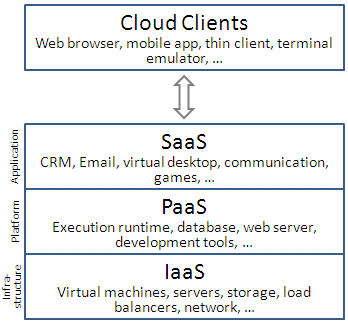
\includegraphics[width=0.6\textwidth]{./images/Cloud_computing_layers.png}
\caption{Cloud computing layers}
\label{F:cloudComputingLayers}
\end{center}
\end{figure}

Moreover, there are different deployment models depending on the product behind (e.g.: specific service or application), which are the resources from the entity that is offering or using such product. Main deployment models might be:

\begin{itemize}
\item Public: when applications/services run over a network that is open for public use, which may be free. The fact of being public/opened implies much more complexity in terms of security issues.
\item Private: when infrastructure is operated solely for a single organization, whether managed internally or by a third-party, and hosted either internally or externally. This cloud type might be similar in terms of architecture design from the public one.
\item Hybrid: when a composition of two or more clouds (private or public ones) are treated as distinct entities but are bound together, offering the benefits of multiple deployment models. Hybrid cloud allows to extend the capabilities of a cloud service by aggregation, integration or customization with another cloud service.
\end{itemize}

To point out that high-performance computing (e.g.: GPU based clouds \cite{gpu}) and software-defined networking (SDN) could improve solutions to current cloud issues such as security, processing performance and full processing chain control through specific SLAs (Service Level Agreements), among others.

So, in many terms, the cloud concept is a key solution to help media producers create better content more quickly and there are lots of examples to focus on, but lets introduce the ones that tends to flexible and scalable ways to access the benefits that cloud computing brings to media production:

\begin{itemize}
\item Low-cost initial expenditures \hfill 

Media production tends to require an enormous initial investment in technology infrastructure and the technical staff to manage it. In that sense, cloud computing technology offers to the creative industries to ease the need to invest heavily in technology that would rapidly become obsolete. Cloud computing allows the media production industry to provision only the technology they need, when they need it, avoiding excessive CAPEX.

\item Cost forecasting\hfill 

Infrastructure as a Service (Iaas) prices are predictable and granularly treated. It allows prediction on a per project basis with detailed cost analysis precision. As done by many IaaS providers (e.g.: Amazon and Woowza), each resource used in a media production workflow is metered, and companies pay only for what they use.

\item Dynamic infrastructure deployment \hfill 

Cloud computing helps production entities take advantage by the on demand basis applied deployments. Media production companies can quickly provision servers to meet the demands of specific projects and shut them down when they are no longer needed. Moreover, cloud computing provides many infrastructure services such as content storage, transcoding, ingestion, \ldots
\end{itemize}

Moreover, cloud computing can improve media production at many different media services requirements planes, such as:

\begin{itemize}
\item Media asset management
\item Granular costs measurement
\item Cloud transcoding
\item High-speed file transfer
\item Automated content verification
\item Elastic deployment
\item Real-time and full monitoring
\item Video quality control
\end{itemize}

And, expected overall outcomes might be:

\begin{itemize}
\item Increased performance
\item Lowered costs
\item Improved cross collaboration
\end{itemize}

As a subchapter corollary, figure \ref{F:cloudComputingLayers} describes generic cloud computing layers, but it also refers to this thesis's topics in order. These are virtualization, monitoring concepts and the service that is going to be deployed and tested which is implemented using the LiveMediaStreamer framework.

\subsection{Virtualization}\label{SOA:Virtualization}

Cloud computing is usually strongly related and implemented with different kinds of virtualization. Many virtualization methods are commonly implemented at datacenters where platforms and services are going to be deployed over different infrastructure architectures. Nevertheless, deploying virtualization at data centers doesn’t automatically mean running over a cloud and it’s possible to deploy clouds without virtualization. Furthermore, as well as cloud computing concept started to be widely used from 2000's, virtualization  technologies can be traced back to the 1960’s such as virtual desktops, but others can only be traced back a few years, such as virtualized applications.

Specifically, virtualization under computing environments means creating a virtual version of any possible piece of actual hardware or software so that we can use system resources effectively. Despite of many ways to define current virtualization methods, the following statement is proposed and it is defined by types and levels:

\begin{itemize}
\item Types: based on specific computer/server resources virtualization. These are: 
\begin{itemize}
\item Data virtualization: when an application is able to retrieve and manipulate data without requiring technical details of such data.
\item Memory virtualization: when, in a cluster, volatile random access memory (i.e.: RAM) resources are decoupled from physical machines in order to be aggregated with other RAM resources and to become a virtualized memory pool.
\item Network virtualization: when combining hardware and software network resources and network functionalities into a single and software-based management entity.
\item Storage virtualization: when pooling data from multiple and different storage devices into a virtual device that is managed from a central console.
\end{itemize}
\item Levels: based on abstract and generic virtualization concepts. These are:
\begin{itemize}
\item Application virtualization: when encapsulating an application software from the underlying operating system on which it is executed. It involves separating the physical client device from the management of the application itself.
\item Environment virtualization: when virtualizing at operating system level. It is a virtualization method where the kernel of an operating system allows for multiple isolated user-space instances, instead of just one. 
\item Hardware virtualization: when hiding the physical characteristics of a computing platform from a user point of view and showing another abstract computing platform. It means computer or operating system virtualization by creating virtual machines.  Nowadays, the software that manages virtualization is called hypervisor or virtual machine monitor.
\end{itemize}
\end{itemize}

Therefore, in terms of cloud computing benefits, virtualization can increase agility, flexibility, and scalability while creating significant cost savings. Workloads might be deployed faster, performance and availability increases and operations can become fully automated, resulting in a cloud with ease to be managed. 

Although the virtualization types that are defined, this subchapter is focusing on the previous defined virtualization layers, which are of interest for this thesis development.

So, starting from the upper layer, application virtualization's current technologies are:

\begin{itemize}
\item Desktop virtualization: when separating part or all of the desktop environment and associated applications from the physical client device that is used to access remotelly or locally it. This improves portability, manageability and compatibility of a personal computer's desktop environment. A common implementation of this approach is to host multiple desktop operating system instances on a server hardware platform running a hypervisor. This is generally referred to as Virtual Desktop Infrastructure (i.e.: VDI). Some commercial examples are RemoteApp of Microsoft and the Seamless Windows of Citrix. 
\item Application streaming: when delivering pieces of the application's code, data, and settings when they're first needed, instead of the entire application being delivered before startup. Running the packaged application may require the installation of a lightweight client application. Packages are usually delivered over a protocol such as HTTP, CIFS or RTSP. Some examples are Microsoft App-V and Citrix XenApp Streaming.
\end{itemize}

Next layer is the intermediate layer of environment virtulization. Pioneer implementation was FreeBSD jails mechanism allowing system administrators to partition a FreeBSD-based computer system into several independent mini-systems called jails. There are many other examples of environment virtualization, but all of them are OS-based virtualization with differences like its kernel operating system (i.e.: FreeBSD, Solaris, Unix-like, and Windows) and the level of isolation in terms of resources utilization (i.e.: types of virtualization, above explained), security and ease of delegation. 

Currently, the environment virtualization method of Linux containers (LXCs) are widely enhancing application/services development, testing, packaging, deployment and managing methodologies. Specifically, containers represent one of the leading trends in computing today. With companies such as Docker, CoreOS, ClusterHQ joining industry giants like IBM, Red Hat, MIcrosoft and others.

Finally, the lower environment virtualization layer is the hardware-centric one. Different methods can be distinguished as follows:

\begin{itemize}
\item Full virtualization: when simulating enough hardware to allow using an isolated guest operating system in a virtual machine. There are many examples of implementation like Parallels, VirtualBox, OracleVM, VMware and QEMU among other platforms.
\item Hardware-assisted virtualization: is a full virtualization enhancement that uses specific hardware capabilities by improving hardware simulation efficiency. There many implementations' examples like Linux KVM and Xen among others platforms. 
\item Partial virtualization: was the previous virtualization technology of the full virtualization. Main differences resides on the address space virtualization, in which each virtual machine consists of an independent address space. This fact implies that a full operating system is not able to run in a virtual machine but many of its applications. 
\item Paravirtualization: when a virtual machine does not implement full hardware virtualization, but offers a special API for a guest with a modified version of the operating system. This type of virtualization is also implemented in most of the widely used virtualization platforms like VMware, Parallels and Xen.
\end{itemize}

\subsection{Monitoring}\label{SOA:monitoring}

Strongly related to cloud reliability is the monitoring concept. In order to reach maximum cloud reliability it is important to observe and check the progress and/or quality of key parameters over certain periods of time and to keep them under systematic review in order to create proper reactions, if required.

Therefore, this implies monitoring the cloud infrastructure (e.g.: servers, virtual or physical) and related services (e.g.: applications). Here appears the QoS (Quality of Service) and QoE (Quality of Experience) terms, respectively.

QoS is the network-centric monitoring of underlying infrastructure components such as servers, routers and its network traffic. QoS metrics are generally device (e.g.: CPU and memory load, CPU temperature, disk space or HDD health) or transport-oriented (e.g.: packet loss, delay, bandwidth usage or jitter). 

Although QoS can be fully affordable due to the robustness and redundancy of current infrastructures (e.g.: back-up services, network rerouting and error correction), this doesn't mean that any end user might be feeling comfortable by using deployed services (e.g.: searching on a e-commerce webpage) over a high QoS infrastructure. Then, QoE monitoring term evaluates the quality delivered to a user and it is done by analysing parameters when connecting to such services like a user. Therefore, QoE performance indicators are user-centric (e.g.: webpages response time or measuring video and audio quality (e.g.: Mean Opinion Score test, MOS)).

Common network monitoring protocols for distributed infrastructures management are:

\begin{itemize}
\item SNMP: Simple Network Management Protocol is a widely known and used Internet standard protocol for managing IP-capable devices. SNMP is based on monitoring stations (i.e.: traps) which implement registry (i.e.: MIBs) polling to specific equipments (IP-capable devices supporing SNMP), which offer data of interest such as disk usage, link status, CPU usage,\ldots Moreover, it can be configured in an asynchronous mode.
\item WMI: Windows Management Instrumentations is a Microsoft's implementation of the Web-Based Enterprise Management (WBEM) and Common Information Model (CIM) standards from the Distributed Management Task Force (DMTF). It offers a detailed set of properties and methods (offering data metrics similar as done by SNMP) for access by an authenticated user but it is all done through Windows proprietary definitions.
\item NetFlow: a Cisco protocol for network switches and routers. It is meant to be used as a network flow analyser (by identifying and analysing each configured flow, which is an unidirectional statistical packet sequence) 
\end{itemize}  

Usually, these protocols are used to measure QoS, but there are complex algorithms that processes those QoS measurements parameters of interest in order to measure the QoE too. Nevertheless, there are specific applications to define and perform specific QoE measurements. 

Focusing our attention in what this thesis is about, the QoE measurements are relevant for audiovisual content services because bad network performance may highly affect the user's experience. This is mainly because these contents are compressed and coded, and have low redundancy. Moreover, when designing systems, for referenced analysis, several elements in the video production and delivery chain may introduce distortion by degrading the content (i.e.: from the transcoding system, transport network, access network, home network to end device).

On the other hand, the referenceless\footnote{Referenceless analysis is a technique studied and implemented by the AGH Multimedia Team \cite{AGHTEAM} and it has been applyed within European projects \cite{mitsu} where i2CAT Foundation's Media Internet area and AGH Multimedia Team has been collaborating \cite{AGHQOE}.} analysis is based on the idea that end users do not know about the original content. In this case, instead of measuring the QoE by comparing the original data to the delivered one, this is done by trying to detect artefacts (i.e.: blockiness, blur or jerkiness for video frames).

Obviously, the automation of critical cloud performance monitoring tasks is crucial for ensuring availability, providing efficient services and reducing common errors, costs and complexity. So, the use of OTT applications that processes such quantities of data flows and displays outcome parameters of interest are crucial. 

There are many tools that offer monitoring capabilities to be integrated and of-the-shelf. Such monitoring capabilities can be organized as:

\begin{itemize}
\item System monitoring \hfill

Single server/computer/instance resources monitoring (e.g.: CPU and memory loads or processes utilization). Typical examples are the system monitoring tools that each operating system comes with by default.
\item Network monitoring \hfill

Related to previous item, but specific to network resources monitoring (e.g.: monitoring input and output accumulated bytes of a single computer network interface or monitoring specific network hardware like accumulated incoming UDP packets of a router in a LAN). There are many examples of tools and services for network monitoring which goes from desktop applications (e.g.: netstat) to specific router and switch daemons (e.g.: MRTG).
\item Infrastructure monitoring \hfill

When coupled system and network monitoring together by adding specific tools and interfaces to monitor distributed resources within the infrastructure. There are many examples of tools  (e.g.: cacti or monitis) and services (e.g.: new relic or pingdom) at this monitoring level.
\end{itemize}

The associated database model for collecting such amount of data is the widely known Round Robin Database, which stores data in a circular buffer based database where the system storage remains fixed by handling time-series data. 

Finally, to remark that network managers have the capability to minimize the storage and network resources by allocating only the resources that are required thanks to monitoring evaluation services and tools.
 
\section{LiveMediaStreamer framework}\label{SOA:LMS}

This section is devoted to the framework which the core service (i.e.: audio and video mixer software) to be analysed is implemented with, the LiveMediaStreamer (LMS) framework. 

The aim of LiveMediaStreamer framework is to offer multiple audio and video streams manipulation in real-time in many ways. It is designed following a pipeline pattern so that it consists in a number of filters (i.e.: encoders, decoders, receivers, transmitters, dashers, mixers and resamplers) that can be concatenated or connected with each other in order to process a data flow. The framework is developed under a Linux environment, currently being the only supported platform, using C++ standard libraries and it makes use of several mature media related libraries, which are: 

\begin{itemize}
\item Live555 \cite{l555} – Network streaming media library which implements the RTP standard protocol.
\item ffmpeg \cite{ffmpeg} – A complete, cross-platform solution to record, convert and stream audio and video.
\item OpenCV \cite{opencv} – Open source computer vision and machine learning software library.
\item x264 \cite{x264} – Free software library and application for encoding video streams into the H.264/MPEG-4 AVC compression format.
\item x265 HEVC Encoder \cite{x265} – Open source HEVC encoder.
\item LAME \cite{lame} – High quality MPEG Audio Layer III (MP3) encoder licensed under LGPL license.
\item Opus \cite{opus} – Totally open, royalty-free, highly versatile audio codec.
\item WebM VPX \cite{webm} – VP8/VP9 Codec SDK. A open, royalty-free, media file format designed for the web.
\end{itemize}
 
The framework is designed to be managed remotely through a simple network interface based on JSON formatted TCP socket messages. 

LMS framework project was stated to be developed since two years ago. A first implementation was based on the network core of the open-source software UltraGrid \cite{ug}. One year after, a new core has been developed based on the network streaming library Live555. This change has improved system performance and eased further developments. Live555 library enables implementing any RTP and RTSP module, standard or not, among offering out of the box specific audio and video RTP payload formats support like H264, HEVC or VP9 for video codecs and G711, OPUS or AAC for audio codecs.

Currently, the framework does not have a RESTful API, but has a web API based middleware, that loads and manages an audio and video mixer scenario, written in Ruby programming language and it implements Sinatra framework for the web service interface side.

To remark that the main reason to provide a REST API is due to its decoupled architecture and low bandwidth usage, which make REST architecture style suitable for developing applications over cloud environments.

Appendix \ref{ANX:lmsarchfull} includes more information about specifics of the LMS architecture in order to understand next chapters (mostly, in problem statement and proposal's subchapter \ref{B:appLayerCH2} and chapter \ref{D:application}, the solution's implementation).

Finally, to point out that there are many existing similar solutions but most of them are proprietary or closed solutions (i.e.: Wowza Streaming Engine or Adobe Flash Media Server). Moreover, if they are aimed to be used as real-time media productions tools they require for external solutions to provide video and audio mixing features.

\chapter{Problem statement and proposal}\label{B:problemStatementAndProposal}

As this title's chapter sample, the aim of this section is to provide a structured vision of the specific problems of each issue to be developed during this project.

Main issues are about to prepare and/or adapt current technologies to be ready for a cloud deployment. This fact implies studying existing technologies and tools in order to create specific microservices that will be interconnected between them. And, finally to carry out required developments in order to assure the goals behind and ease demonstrate the results.

--------- splitting the current interface of HTTP requests to TCP socket messages, this means creating the API middleware service that will let configure specific LiveMediaStreamer instances  that loads the audio and video mixer scenario-----------

\section{Architecture study}

Therefore, above all it's required to define the platform's architecture to prototype in order to have a global and generic insight. So, taking into account the pieces required for this project (i.e.: service layer, monitoring layer, virtualization/deploy layer), such architecture should contain the different high level layers as shown next:
\begin{figure}[htb]
\begin{center}
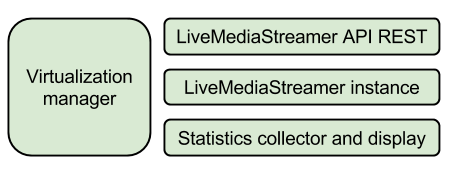
\includegraphics[width=0.4\textwidth]{./images/generalArch.png}
\caption{Generic platform architecture}
\label{F:genericPlatArch}
\end{center}
\end{figure}

The "LiveMediaStreamer API REST" layer will contain the service that will be offered to different and external applications in order to manage the "LiveMediaStreamer instance" layer by creating different audio and video production scenarios. Both layers are the core layers of the platform.

Moreover, in order to offer a centralized monitoring system, the "Statistics collector and display" layer becomes as the generic box for this requirement.

Finally, it is also required to provide an orchestrator that manages the deployment and distribution of the possible configurations for the previous introduced layers. This will be done thanks to the "Virtualization manager" layer.

\subsection{Virtualization}

This subsection aims to introduce the possibilities that different virtualization technologies could offer for this project requirements and to decide between one of them.

First of all, next points are showing which are the expected outcomes for using virtualization and what should fulfil the selected technology:

\begin{itemize}
\item To manage and maintain a system of small pieces of services (assure a microservice architecture based pattern)
\item To have flexibility in order to quickly load (e.g.: start, restart, stop) required instances (e.g.: to assure real-time scalability) and to deploy any possible required scenario/configuration.
\item To offer ease to continuous develop and deploy the different parts of the architecture
\item To have version like system for having different version tags for the architecture modules (e.g.: a development and a production box of the same API REST service)
\item To assure full compatibility for the core layers' operating system (right now only Linux environments are supported)
\item To assure full compatibility for the hardware to work with (mainly x86 processors are in the scope)
\end{itemize}

Therefore, it is also required to use an as much lightweight as possible technology.

Under Linux environments there are many virtualization options (most of them proprietary) to analyse, but lets focus on the ones that are open-source and have wider and active communities behind.

These are KVM with QEMU and LXC with Docker:

\begin{itemize}
\item KVM (Kernel-based Virtual Machines) \hfill

It's a FreeBSD and Linux kernel module that offers a full virtualization solution for Linux on x86 hardware containing virtualization extensions (Intel VT or AMD-V). It consists of a loadable kernel module that provides the core virtualization infrastructure and a processor specific module.
Usually, KVM runs with the QEMU (Quick Emulator) which is a complete and standalone emulating suite that performs hardware virtualization.

KVM with QEMU is able to offer virtualization for x86, PowerPC, and S/390 guests. For instance, when the target architecture is the same as the host architecture, QEMU can make use of KVM particular features in order to do not emulate CPU nor memory.
\begin{figure}[htb]
\begin{center}
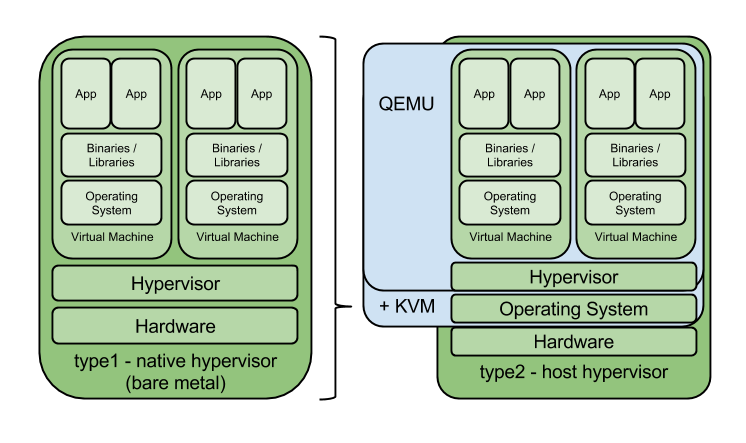
\includegraphics[width=0.5\textwidth]{./images/KVM.png}
\caption{QEMU with KVM or hypervisor type2 to type1}
\label{F:KVMandQEMU}
\end{center}
\end{figure}

Previous figure \ref{F:KVMandQEMU} showcases how KVM can convert a type2 hypervisor (i.e.: QEMU) into a type1 hypervisor (known as a bare metal hypervisor) which increases overall application performances. 

\item LXC (Linux Containers) \hfill

It's an operating-system-level virtualization environment for running multiple isolated Linux systems (known as containers) on a single Linux central host.

Linux kernel itself provides the cgroups functionality that allows limitation and prioritization of resources (CPU, memory, block I/O, network, etc.) without the need for starting any virtual machines, and namespace isolation functionality that allows complete isolation of an applications' view of the operating environment, including process trees, networking, user IDs and mounted file systems.

Nowadays virtualization tendencies are focusing on the Docker project, which is a platform that provides an additional layer of abstraction and automation of operating-system-level virtualization on Linux, Mac OS and Windows.
\begin{figure}[htb]
\begin{center}
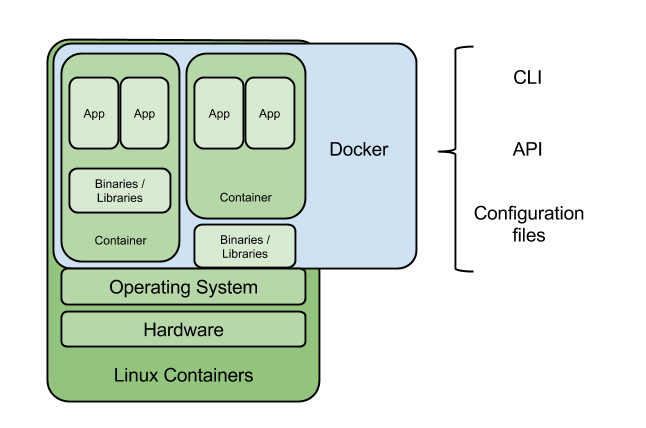
\includegraphics[width=0.5\textwidth]{./images/LXC.png}
\caption{Docker with LXC}
\label{F:DockerAndLXC}
\end{center}
\end{figure}

LXC with Docker mean resource isolation features of the Linux kernel to allow independent containers to run within a single Linux instance, avoiding the overhead of starting and maintaining virtual machines. Moreover, Docker project automates the deployment of applications inside software containers and offers different tools to manage them (i.e.: CLI, API and file configurations), as shown in figure \ref{F:DockerAndLXC} 
\end{itemize}

Thus, it seems that the technology that best suits this project requirements is the Docker project. Main reasons are the capabilities of ease maintain, test and quickly deploy each container. Moreover, ---APENDIX X--- demonstrates that the performance offered in front of the Virtual Machine (i.e.: QEMU + KVM) one is rather better.

\subsection{Monitoring layer}

\subsection{Application layer}


\section{Architecture proposal}
\section{Task planning}




\chapter{Application}\label{D:application}

This chapter aims to develop the tasks introduced for the application layer in this project Gantt (see figure \ref{F:tpgp}).

\section{REST API}

As mentioned previously, it's required to develop an API ready to be used over cloud environments in order to ease creating specific and new applications over the LMS framework, and thus to demonstrate the viability of this project prototype.

Nowadays, the common and widely used format for cloud services intercommunication is JSON, as it is also used for the TCP socket API of the LMS framework. Therefore, this API middleware is going to follow such premise.

A suitable technology to work with JSON formatted messages which is widely known for its good performance is Node.js \cite{nodejs}. Node.js is an open source, cross-platform runtime environment for server-side and networking applications. It provides an event-driven architecture and a non-blocking I/O API that optimizes application's throughput and scalability. This technology is commonly used for real-time web applications. 

Moreover, working with Node.js means avoiding serialization of the JSON messages by increasing services intercommunication performance (i.e.: less computational cost and less processing time). 

Then, the common Noje.js framework for developing web applications and REST APIs is Express.js \cite{expressjs}. It's the de facto standard server framework for Node.js. So, the middleware to develop is going to use its routing system, which refers to the definition of end points (URIs with HTTP request methods like GET, POST, PUT and DELETE) to an application and how it responds to client requests.

Following is the software structure proposal for developing the HTTP RESTfull API middleware, which is responsible to translate to the TCP socket API of the LMS framework:

\begin{figure}[!htb]
\begin{center}
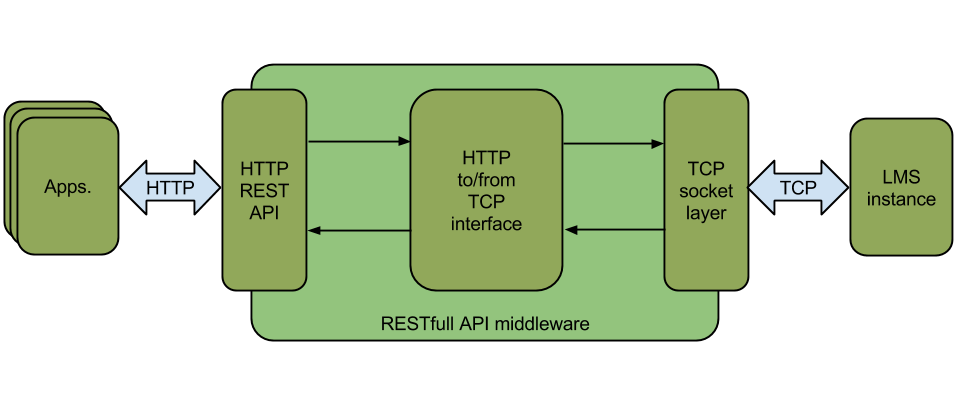
\includegraphics[width=1\textwidth]{./images/RESTAPI.png}
\caption{RESTfull API middleware architecture}
\label{F:restAPI}
\end{center}
\end{figure}

\begin{itemize}
\item HTTP REST API layer \hfill

This layer handles HTTP queries from external applications. It implements specific routes to handle specific HTTP queries. First implementation will not implement multiple LMS management but single. As shown in figure \ref{F:restAPI}.

\item Interface layer \hfill

This layer handles the body messages from the previous layer's HTTP queries and manipulates them in order to create an as much generic as possible API by adapting the messages to be sent through following layer.

\item TCP socket layer \hfill

This layer is the responsible to send and receive JSON formatted TCP socket messages between the LMS instance targeted.
\end{itemize}

As introduced in section \ref{SOA:LMS} and deeply explained in APPENDIX \ref{ANX:lmsarchfull}, there are two different management layers: the generic and the filter specific. So, by following this organization, the proposed API's structure is as shown in APPENDIX \ref{ANX:RESTAPI}.

To point out that this API is not implementing persistence because the state (managed through 'State' method) is given by the LMS instance itself. The unique sign of persistence is regarding the LMS host and port which the middleware is connected to (managed through 'Connect' and 'Disconnect' methods). Higher levels of persistence should be implemented by external applications which implies specific scenarios and requirements (i.e.: specific persistence).

Finally, in order to know how this structure and the overall middleware is implemented check APPENDIX \ref{ANX:sourceCodes} to see the code. Next chapters will demonstrate it too.

\section{Network metrics}

Network metrics could be treated as external metrics. This is because these metrics are specially dependent from sources which transmit to LMS, the receivers from LMS and the state of the network itself. Obviously, the performance of the LMS affect to the metrics gathered too, but it is intended to be minimized, at least in a gathering and presentation of the metrics' point of view.

\subsection{Input network metrics}

As said in subsection \ref{B:appLayerCH2}, input network metrics are going to be implemented by carrying out methods re-implementations given by the Live555 library, which is the library implemented for managing network streams.  

\begin{figure}[!htb]
\begin{center}
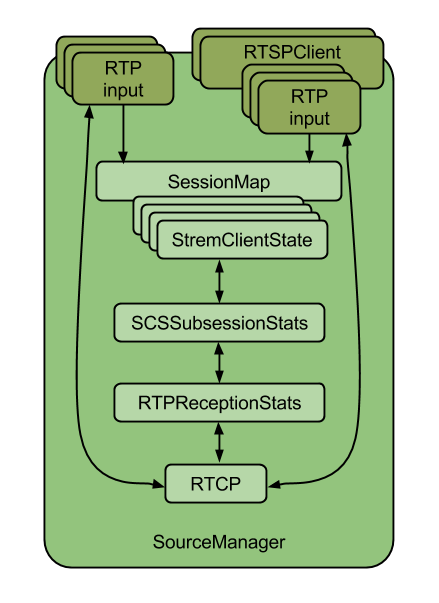
\includegraphics[width=0.45\textwidth]{./images/SourceManager.png}
\caption{Input network metrics structure}
\label{F:inms}
\end{center}
\end{figure}

By following the LiveMediaStreamer architecture structure, input network implementations are going to be implemented inside the 'liveMediaInput' structure. Concretely, a new class is implemented, called 'SCSSubsessionStats'. This class is managed by the 'StreamCleanState' class which is a class related to each stream 'Session' class managed by the 'SourceManager' class. This last class is a 'HeadFilter' class. Figure \ref{F:inms} shows the inter-class structure.

By initializing new RTP or RTSPClient sessions (i.e.: network inputs), a group of subessions is associated per each stream (i.e.: an RTP session has one subsession associated and the RTSPClient session has as many subsessions as accepted from the SDP that defines different RTP sessions).

When a new subsession is set, then, automatically, a new RTPReceiverStats class is initialized. This Live555 object implements RTCP stats measurement which are only required to be treated outside. This is done at SCSSubsessionState, which creates a new schedule to periodically measure and save current state (a default granularity of 1 second is set).

The implemented method that is called periodically is as shown in APPENDIX \ref{ANX:appALG} section \ref{inmm}.

Previous algorithm prepares the metrics that are going to be presented through the state when a new state query is received. In the code is shown how metrics from Live555 library are obtained. For a more detailed insight of the overall implementation see APPENDIX \ref{ANX:sourceCodes}. Next are listed the metrics that are presented per each new state query:

\begin{itemize}
\item Bitrate: maximum, minimum and average in kbps.
\item Packet loss percentage: maximum, minimum and average.
\item Inter-packet gap: maximum, minimum and average in milliseconds.
\item Jitter: maximum, minimum and current inter-packet gap variation in microseconds.
\end{itemize}

All these metrics are measured through previous algorithm shown which is scheduled each second (it is the default value set for all metrics gathered indeed). Concretely the bitrate is measured by knowing the overall number of octets (i.e.: bytes) received during each scheduled period and the elapsed time given by the Live555 library implementation:

\begin{equation}\label{E:bitrate}
average\ bitrate (kbps) = 8 \cdot \frac{kbytes\ receivd\ now}{elapsed\ seconds}
\end{equation}

Moreover, the maximum and the minimum are the last maximum and minimum average bitrates obtained, and this is done for all other metrics.

Then, it is important to remark that the jitter is measured as the estimate of the statistical variance of the RTP data interarrival time to be inserted in the interarrival jitter field of reception reports (in microseconds), and this is already internally done by the Live555 library. So, what is presented is the current jitter value at the beginning of each new schedule.

Another metric that might be of interest is the time delay from the stream source but it is discarded due to not being offered from Live555 library. Moreover, to be implemented at SCSSubsessionStats class level has been discarded due to is computational cost and complexity to develop such requirement. But, to point out that it is not a high priority required metric due to take into account that this issue is out of LMS performance scope and if there are network performance problems they can be detected through other metrics already gathered.


\subsection{Output network metrics}

As done in previous section, output network metrics are going to be implemented by carrying out methods re-implementations given by the Live555 library, which is the library implemented for managing network streams.

This implementation has been much more difficult to be achieved due to not having control of the RTPSink class of the Live555 library in the sense that when it is created neither deleted. Previous developments before the final version where based over the RTPSink re-implementation already done per each OnDemandServerMediaSubsession (Live555 library class), which is also re-implemented by QueueServerMediaSubsession (LMS framework class). But the implementation was still losing the specific RTPSink instance of specific subsession.

In order to go on the development an e-mail was sent to the Live555 developers mailing list, concretely to the head developer of the library, thanks to his replay the solution was clarified (see APPENDIX \ref{ANX:emailRoss}).

So, the best option, as suggested by Ross, was to re-implement the RTCPInstance class per each inheriting class of the OnDemandServerMediaSubsession class, concretely the inheriting classes of the QueueServerMediaSubsession class. 

\begin{figure}[!htb]
\begin{center}
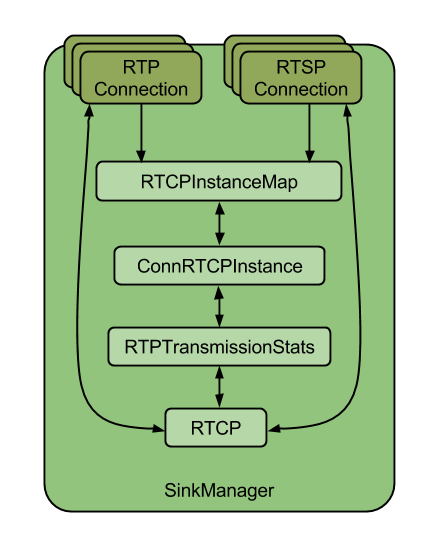
\includegraphics[width=0.45\textwidth]{./images/SinkManager.png}
\caption{Output network metrics structure}
\label{F:onms}
\end{center}
\end{figure}

In figure \ref{F:onms} is shown the relationship between the SinkManager class with both possible types of connections (i.e.: RTP or RTSP). Each Connetion object has a map of objects of the re-implemented RTCPInstance class, called ConnRTCPInstance (i.e.: RTCP instances per each connection). Then, each time a new specific RTP connection or any QueueServerMediaSubsession (RTSP connection, from RTSP server) is created, a ConnRTCPInstance is associated in order to start gathering the statistics offered from Live555 library. This is shown in APPENDIX \ref{ANX:appALG} section \ref{onmm} piece of code by showing the method which is periodically called (default periodicity value is set to 1 second), as done for the input network metrics.

In this case, the delay metric is offered from the Live555 library, which is gathered.

Finally, presented metrics are as shown next:

\begin{itemize}
\item Bitrate: maximum, minimum and average in kbps.
\item Packet loss percentage (ratio): maximum, minimum and current.
\item Round trip delay: maximum, minimum and current in milliseconds.
\item Jitter: maximum, minimum and current inter-packet gap variation in microseconds.
\end{itemize}

All these metrics are measured by applying the same patterns as done for the input network metrics.

\section{Pipeline metrics}

Following metrics are intended to be exposed as the internal metrics. It's important to point out that the measurements behind are really responsive to the overall performance of the LMS framework. Therefore, to achieve the minimum computational cost is a must. Then, as introduced in subsection \ref{B:appLayerCH2}, the optimal solutions to gather and measure such metrics is as shown next. But, first of all, let's pick up the example figure of a pipeline from APPENDIX \ref{ANX:lmsarchfull} in order to showcase the internal pipeline structure of the LMS framework. This will help understanding next two implementations.

\begin{figure}[!htb]
\begin{center}
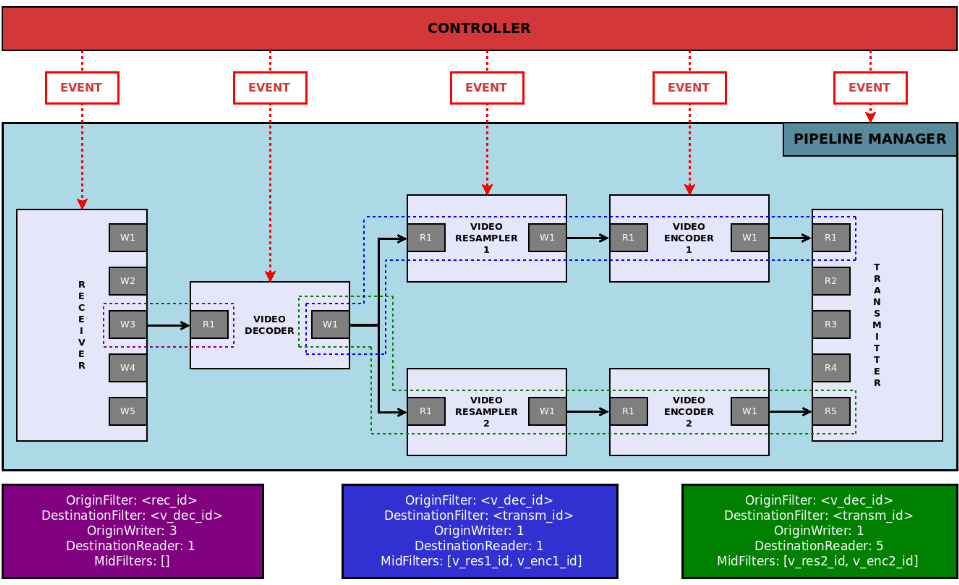
\includegraphics[width=0.9\textwidth]{./images/LMSpipelineBasicOne.png}
\caption{LMS framwork's internal pipeline structure example}
\label{F:lmsps}
\end{center}
\end{figure}

To point out that in figure \ref{F:lmsps} the arrows are the queues which interconnect each filter's writer with another filter's reader. Writers and readers are subclasses of the IOInterface class.

\subsection{Delay}

First of all, to emphasize that this metric is related to the time which data (i.e.: a video frame, an audio sample,\ldots) takes to be processed from an origin point to an end point by an unique given path, and this is measured thanks to a given and required time: the data's timestamps. Data inside the LMS source code is known as a "frame", which can be an audio frame (i.e.: sample), a H264 NAL unit, a raw frame, \ldots 

The delay time isn't considered to be measured per each filter in order to not affect the overall performance but each measured time involves an origin filter which resets the timestamps. These origins are the Head (i.e.: receiver filter) and OneToMany (i.e.: audio and video mixer filters) filters. These filters reset the frames' timestamps in order to reach and control an internal synchronization, and this is due to the fact that these filters have many outputs (i.e.: writers) or many inputs (i.e.: readers) and they require synchronizing their outputs in order to assure one point of time control inside the LMS framework, whatever the scenario configured.

So, in order to measure the delay it is important to note that a pipeline isn't composed by an unique path (see APPENDIX \ref{ANX:lmsarchfull} for clarifications) but multiple paths. This fact implies that it's not possible to measure an unique overall delay time per frame which goes over the pipeline (indeed there is a special case, and this is when there is a unique path that defines the pipeline itself, an unique path), or at least it's not suitable for performance issues, but it can be done for external applications which know the scenario configuration and gathers such metrics. Therefore, this is solved by splitting the measurements by paths. And this is an optimal measurement: the delay is given by the differential time measured by the last reader of the path (i.e.: the reader of the destination filter).

In APPENDIX \ref{ANX:appALG} section \ref{pdmm} is shown the method which implements the measurement inside the Reader class.

So, what is done is to measure the average delay of a frame by a given window time (default is configured to 1 second) with a resolution of microseconds. And this means measuring from the origin time, which, as said, is set by the origin filters (i.e.: the beginning of a path, starting from a writer), to each reader of the path (i.e.: each filter). But, the delay time presented is from the beginning (i.e.: initial writer of the path) until the last reader. See figure \ref{F:lmsps} where different path examples are illustrated.

\subsection{Losses}

This metric is following a similar criteria as the previous one. This is solved by measuring at the same point, but it's done when flushing frames at the reader side (as introduced in section \ref{B:appLayerCH2}). In order to reach minimal computational cost, the measurement is just a counter of the overall data losses when calling the flush methods. What is done is a method encapsulation by defining a parent method that is just incrementing its reader counter and then it calls the specific flush implementation per each data/frame type.

Then, in order to properly present it to external applications it is required to be presented at a path level as done for the delay metrics. So, in this case it is only required to sum up the overall losses of the path's readers.

It is important to note that this metric is not referenced to a total data processed or at any time point, but specific problem detections are achieved thanks to measuring its continuity. This means that if this value is incrementing gradually then the system is not working properly. Such detections might imply fast increments on its continuity (differential increase). 


Finally, as a section corollary, Pipeline metrics are measured when flushing frames (discarding) or when a reader is able to remove a frame from its belonging queue. 

\chapter{Virtualization}\label{D:virtualization}

This chapter focuses on the preparation of generic containers for a media production platform prototype with the technologies and tools introduced in Chapter \ref{A:stateOfTheArt}. We study and test the Docker technology in order to assure that LMS is ready to properly fit in a containerized environment and to evaluate different possibilities to reach maximum flexibility when configuring and deploying different scenarios.

\section{Creating and managing generic containers}
The minimal containerized entities are the following ones:

\begin{itemize}
\item The core container with a LiveMediaStreamer instance already deployed inside and ready to use.
\item The HTTP REST API container with the middleware interface inside and ready to use
\end{itemize}

First of all, let us introduce how and where Docker is installed. The host operating system where tests are going to be carried out is an Ubuntu 14.04 LTS \cite{ubuntu}, which is the Linux distribution version where the LMS is being developed. Note that previous list does not handle monitoring requirements, but this topic will be treated in Chapter \ref{G:monitoringLayer}. this is because our initial interest is related to testing how LiveMediaStreamer can be deployed inside a containerised environment.

Note that main Docker requirements for Ubuntu 14.04 are to be under a 64-bit installation and kernel must be at version 3.10 or higher (lower versions are buggy and unstable). 

Some procedures must be taken into account in order to properly install and assure a best fit possible of the Docker technology inside the OS (and also to be ready for a cloud environment). These procedures include:

\begin{itemize}
\item To create a docker group: in order to avoid user permission issues.
\item To adjust memory and swap accounting: in order to not suffer memory overhead and performance degradation.
\item To enable UFW forwarding: if UFW is enabled it is required to properly configure its forwarding policy (if UFW's enabled it will drop all forwarding and incoming traffic).
\item To configure a DNS server: since Docker defaults to using an external DNS nameserver, it cannot use the local one.
\end{itemize}

It is strongly recommended to check documentation's web page of the official Docker project site \cite{docker} in order to know how these configurations can be done.

Once Docker is properly installed as a daemon in the OS let us focus on interesting possibilities that this technology offers in order to create and manage containers:

\vbox{\begin{itemize}
\item Creating containers
	\begin{itemize}
	\item Using a Docker file \hfill
	
	This is the main configuration file for a Docker container set up. It can be seen as an initial script to build a specific docker container. Also, it is like setting up a local git\footnote{Git is a version control system for software development. It is a distributed revision control system.} repository to later distribute it, but at a container level instead of software level. There you can define many configuration parameters in order to install and properly configure required dependencies and tools to run inside. 	
	
	\item Using Docker pull, commit and push for images

	This is not recommended for creating an original container, but it is appropriate when starting with Docker technology. However, it is recommended to be used once an initial container has been build (from a Docker file) in order to maintain and to distribute different versions and deployments of this (as said, as a higher level git repository).	 
It is important to note that a Docker image consists of a series of layers. Docker makes use of union file systems to combine these layers into a single image (the container itself). Union file systems allow files and directories of separate file systems, known as branches, to be transparently overlaid, forming a single coherent file system. This last fact is a key point due to its capacity of also offering deployment layers inside a container (i.e.: more than one tool/technology inside a container).
	
	\end{itemize}
\item Managing containers 
	\begin{itemize}
	\item Using Docker Hub service

	It is a public registry of Docker images' repositories (there are also private ones with specific paying plans) from Docker official site. There is a list of basic (e.g.: CentOS, Ubuntu, Debian, ...) and complex (e.g.: CentOs with Nginx, Ubuntu with Nginx and Wordpress, Debian with Node.js and MongoDB, ...) containers containing clean and/or OS environments. 
	
	\item Using Docker Registry and Repository service

	This item is a key point when looking for local management of images' repositories. This tool let us deploy an external (e.g.: private) registry if some enhancements over Docker Hub are desired (e.g.: specific user credentials, high level security layer,...).
	
	\item Using Docker Compose
	
	This tool let us create a localhost orchestrator of docker containers. This means managing/running more than one container and linking them (if required) at same time from the same point.
	
	\end{itemize}
\end{itemize}}

For a more specific detailed list of options and possibilities from Docker containers, please check Appendix \ref{ANX:csd}.

\subsection{Basic LMS container}

Once previous brief of Docker possibilities to work with has been introduced let us start containerizing a single LiveMediaStreamer.

As shown in the wiki page at GitHub's LiveMediaStreamer (see Appendix \ref{ANX:lmsarchfull}), the framework has some requirements and dependences that should be previously solved (i.e.: installed). Appendix \ref{ANX:dockerFiles} Section \ref{ANX:dockerFiles1} lists the first and basic Docker file which installs and configures the image in order to run a LMS instance. 

Now, let us focus on what is done in order to explain it better: 

\begin{itemize}
\item FROM: this command indicates which is the image base to be used, in this case, as previously mentioned, Ubuntu 14.04 is the selected environment.
\item MAINTAINER: this command tags the maintainer/creator of such container image.
\item RUN: specific command which runs specific bash scripts (e.g.: apt-get, mkdir, adduser and any other available system command from the base image)
\item USER: this command is used in order to specify the system user that is going to be loaded in such container. This is mainly for security reasons (e.g.: avoiding root user).
\item EXPOSE: this command handles the ports to be exposed from the container itself. This does not imply that later ports couldn't be exposed through the command line interface, but it is used in order to list suitable ports to be required. In this case, the exposed ports are a range of UDP ports where streams will be input or outputted (i.e.: RTP), a TCP range for the RTSP and the TCP port for managing the LMS framework through TCP socket messages. 
\item CMD: this configures the command that will be executed when running the image itself. It is important to point out that any user can later enter inside the container avoiding the execution of the default CMD defined (e.g.: executing bash for development purposes inside the container and creating a new container's version).
\end{itemize}

There are many other commands that could be used inside a Docker file (see Appendix \ref{ANX:csd}) but they are not required in this case.

Once the Docker file is defined it is time to build the image as follows:

\begin{verbatim}
$ docker build \
		-t <origin repository registry>/<image name>:<version tag> \
		<Docker file folder path>
\end{verbatim}

Note that in order to start working with different images and managing them in different environments (i.e.: different servers/computers) a Docker Hub account has been created. So, let us define each parameter in order to name and tag each image to built during this thesis. In this case:

\begin{itemize}
\item Origin repository registry is "gerardcl" (see \url{https://hub.docker.com/r/gerardcl})
\item Image name is "lms"
\item Image version tag is "single"
\end{itemize}

The last command builds the image by following the defined script inside the Docker file already defined. Finally, the command to execute the image is:

\begin{verbatim}
$ docker run --rm -p <host port>:<container port> \
		--name single-lms gerardcl/lms:single
\end{verbatim}

This last command runs the previous defined and built image by exposing internal TCP port (i.e.: \verb|<container port>|, which has been configured in CMD method with 7777) to another defined TPC port at host side (i.e.: \verb|<host port>|). Flag \verb|--rm| is used in order to be able to run again the same command by defining (i.e.: identifying) the running image with "single-lms" name (i.e.: \verb|--name| flag). Note that for testing purposes flags \verb|-i -t| (or \verb|-it|, it is just the same) might be also added in the command in order to run as an interactive process (this means allocating a TTY for the container process, so exposing the STDIN, STDOUT and STDERR standard streams). Therefore, the effect is similar to executing the process over the same OS too.

Finally, in order to expose other ports it is just required to add the -p flag as many times as ports required. If an UDP port is also required to be exposed it is required to add the udp tag as shown:

\begin{verbatim}
$ docker run --rm -p <host port>:<container port> \
		-p <stream1 host port>:<stream1 container port>:udp \
		--name single-lms gerardcl/lms:single
\end{verbatim}


\subsection{HTTP REST API container}

The following container to be built is the HTTP REST API middleware developed in Chapter \ref{D:application}. Since it is a Node.js application, it requires to be built with Node.js and the NPM which is the official Node.js package manager. NPM is used to to install middleware's dependencies. This is show in Appendix \ref{ANX:dockerFiles} Section \ref{ANX:dockerFiles2}.

In this case, in order to build and manage such image, these are the image parameters which define this image:

\begin{itemize}
\item Origin repository registry is "gerardcl" (see \url{https://hub.docker.com/r/gerardcl})
\item Image name is "lms-rest-api"
\item Image version tag is "single"
\end{itemize}

The building command is:

\begin{verbatim}
$ docker build \
		-t gerardcl/lms-rest-api:single \
		<Docker file folder path>
\end{verbatim}

Note that the middleware implementation support changing the listening port of the application (default is 8080) by just adding the "-e" flag and defining the "PORT" environment variable of the container. An example is shown:

\begin{verbatim}
$ docker run -it -e "PORT=9000" -p 8080:9000 \
		--name lms-rest-api --rm  gerardcl/lms-rest-api:single
\end{verbatim}

This last command sets the internal "PORT" environment variable to 9000 and binds it to the 8080 port of the host.

\section{Linking containers}

In order to play with the previously built containers, it is required to know how they might be interconnected (i.e.: linked).

\subsection{Same OS}

If containers are running on the same OS it is important to keep in mind that each environment is isolated and its network environment is isolated too. Then, in order to let the HTTP REST API container connect to and manage the LMS instance container it is required to share the its network environment with LMS instance container. Here is how each container might be executed:

\begin{verbatim}
$ docker run -it -p 8080:8080 --name lms-rest-api \
		--rm  gerardcl/lms-rest-api:single
\end{verbatim}
\begin{verbatim}
$ docker run -it --rm --net container:lms-rest-api \
		--name lms gerardcl/lms:single
\end{verbatim}

Flag \verb|--net container:<container id>| helps solving this issue. This configures the "lms" container to use the network environment of the "lms-rest-api" container. So, both containers are on the same localhost, but isolated. The only exposed port is the 8080, which is required to get access to REST API.

To point out that in this case it is not required to expose the TCP socket API port because it is internally linked through the REST API container. This is a key point of the Docker technology, which lets isolate a container from external world. 

In order to demonstrate it let us show what a \verb|$ netstat -putaneo| command  execution returns:
\begin{itemize}
\item Looking for port 8080: \hfill

\begin{verbatim}
Proto LocalAddress ForeignAddress State  User  PID/Program name 
 tcp6   :::8080        :::*       LISTEN  0    21735/docker-proxy
\end{verbatim}
\item Looking for port 7777: \hfill

No result obtained so isolation is reached on port 7777
\end{itemize}

\subsection{Separate OS}

In order to deploy each container in separate OS it is required to expose required ports for achieve intercommunication. The Docker "run" command might be:
\begin{itemize}
\item For LMS container (only exposing TCP socket API control ports): \hfill

\begin{verbatim}
$ docker run -it --rm -p 7777:7777 --name lms gerardcl/lms:single
\end{verbatim}
\item For REST API container: \hfill

\begin{verbatim}
$ docker run -it -p 8080:8080 --name lms-rest-api --rm  \
		gerardcl/lms-rest-api:single
\end{verbatim}
\end{itemize}

Then, in order to reach connection from REST API to LMS the host to set in the connect JSON parameter is the host IP of the OS which is running the LMS instance containerized. And, obviously, in order to play with the REST API and control the remote LMS instance, the host URI must be the OS IP of the running REST API container.

\section{Running multiple processes within a container}

Finally, it is important to note that a Docker image is only able to run a single process through the CMD method. But there is a solution to reach executing more than one process (i.e.: multiple services). This fact will help developing Chapter \ref{G:monitoringLayer}.

The solution for running multiple services inside the same container remains on a common and widely used tool, called supervisord. Supervisord is a client/server system that allows monitoring and controlling any number of processes on UNIX-like operating systems, which is meant to be used to control processes related to a project or a customer (i.e.: a Docker container), and is meant to start like any other program at boot time.

An example for supervisor to be required is due to the fact that LMS framework is able to encapsulate audio and/or video streams to MPEG-DASH\footnote{Dynamic Adaptive Streaming over HTTP (DASH), also known as MPEG-DASH, is an adaptive bitrate streaming technique that enables high quality streaming of media content over the Internet delivered from conventional HTTP web servers.} \cite{mpegdash} segments, which a key point feature of the LMS framework in order to offer live or on demand streaming to browser applications. Therefore, in order to let a browser play obtained segments an HTTP server is required, which serves the required files to be sent to the browser. Appendix \ref{ANX:dockerFiles} Section \ref{ANX:dockerFiles3} describes the Docker file for building such container, which will have a LMS instance and a HTTP server (i.e.: Nginx).

This is quite similar to the first Docker file introduced in this chapter but:

\begin{itemize}
\item Nginx and Supervisord are also installed
\item Specific /var/run and /var/log folders are created per each Supervidord process inside the supervisord.conf file
\item This Docker file uses the command ADD in order to add specific configuration files for the Nginx and Supervisord container's servers (they are later showcased)
\item What is executed now is the Supervisord daemon
\item The port for the Nginx server is exposed
\item The user that is going to be used for this container is its root user due to require being used by supervisord service itself
\end{itemize}

The Nginx configuration file is as shown in Appendix \ref{ANX:dockerFiles} Section \ref{ANX:nginxexample}. In this configuration file, apart from typical Nginx configurations (which are out of scope of this thesis), some access control methods are added in order to treat common HTTP server issues like CORS (Cross-Origin Resource Sharing). Note that the root file system specified is the one which the LMS instance should use for saving the MPEG-DASH output files too (i.e.: the dasher filter should be configured with this folder).

Finally, the last file to show is the supervisord.conf configuration file:

\begin{verbatim}
[supervisord]
nodaemon=true

[program:livemediastreamer]
command=/usr/local/bin/livemediastreamer 7777

[program:nginx]
command=/usr/sbin/nginx 
\end{verbatim}

This supervisord configuration file defines both services to be executed, LiveMediaStreamer and Nginx. Then, as done with previous Docker files, let us show how it should be built:

\begin{verbatim}
$ docker build \
		-t gerardcl/lms:dash \
		<Docker file folder path>
\end{verbatim}

An example command to run this container's image is shown next:

\begin{verbatim}
$ docker run -p 8090:8090 -p 7777:7777 -p 5004:5004/udp -it \
		--rm --name lms-dash gerardcl/lms:dash 
\end{verbatim}

So, this container will serve the MPEG-DASH files on http://host:8090/ and it will also be listening on port 7777 in order to get TCP socket configuration messages and it will be listening on port 5004 in order to receive an audio or a video on that port.

\section{Best practices}

As illustrated in the official Docker documentation web site \cite{dockerBP}, one of the best practices that should be taken into account is to avoid creating complex images and try to split as much as possible them.

For example, the previous section is just an example of a scenario where running multiple services inside a container is a must (i.e.: when there are no other options or the solution becomes much complex or the customer demands it), which should be avoided.

So, let us try to showcase a best practice for solving previous use case. By using the "volumes" feature that Docker offers, this last container with multiple services inside could be splitted into two: one specific container for a Nginx server (with same configuration file as shown before) and the other the single LMS container introduced at the beginning of this chapter. 

First of all, let us describe which is the Docker file generated for the Nginx container in Appendix
\ref{ANX:dockerFiles} Section \ref{ANX:dockerFiles4}

Then, the build command might be as follows:

\begin{verbatim}
$ docker build \
		-t gerardcl/lms-nginx:single \
		<Docker file folder path>
\end{verbatim}

Finally, let us show in order which should be the commands to execute:

\begin{verbatim}
$ docker run -v <host volume folder>:/home/lms/dashSegments \
		-p 7777:7777 -p 5004:5004/udp -it --rm \
		--name lmsdash gerardcl/lms:single
\end{verbatim}

\begin{verbatim}
$ docker run -it -p 8090:8090 --rm --name nginx \
		--volumes-from lmsdash:ro gerardcl/lms-nginx:single 
\end{verbatim}

With \verb|-v| flag is specified the "host volume folder", which is the host folder shared with the internal folder which LMS container will write the MPEG-DASH files. If not specified, default permissions are read and write. Then, the Nginx container will use the \verb|--volumes-from <container id>:<permissions mode>| flag by specifying the containers from which will share its volume and its file permissions. In this case file permissions are specified to be in read-only mode in order to not avoid file modifications from the server/container side.  
 
So, scalability, performance and control of the set of containers are assured by applying best practices like the last one.

Finally, to remark that thanks to these illustrations of Docker file configurations there is a step forward to demonstrate this thesis's goals.

\chapter{Monitoring layer}\label{G:monitoringLayer}

As already discussed, in order to properly manage a cloud computing environment it is strongly required to use monitoring tools in order to gather information of interest by improving the environment itself or by finding out issues and solving them as fast as possible.

This chapter aims to showcase how the selected monitoring tools can fit in the architecture type that has been proposed. And, how they can be used. This means, preparing the environment to support Collectd (i.e.: monitoring and gathering) and Graphite (i.e.: storing and presenting) tools.

Moreover, to point out that such tools are helpful to demonstrate that LiveMediaStreamer framework could be deployed as the core of a real-time media production platform (see chapter \ref{H:platformDeploymentAndDemonstrations}).

So, to remark that the fact of creating small and reusable containers is the main goal of this chapter and, of course, the goal of this platform architecture to prototype. And, thanks to the selected monitoring tools, which are lightweight and ease configuration flexibility, this issue might be properly solved.

Then, a proposal of the monitoring architecture in a more detailed description (regarding figure \ref{F:MLAP}) is shown in figure \ref{F:maex}.

\begin{figure}[htb]
\begin{center}
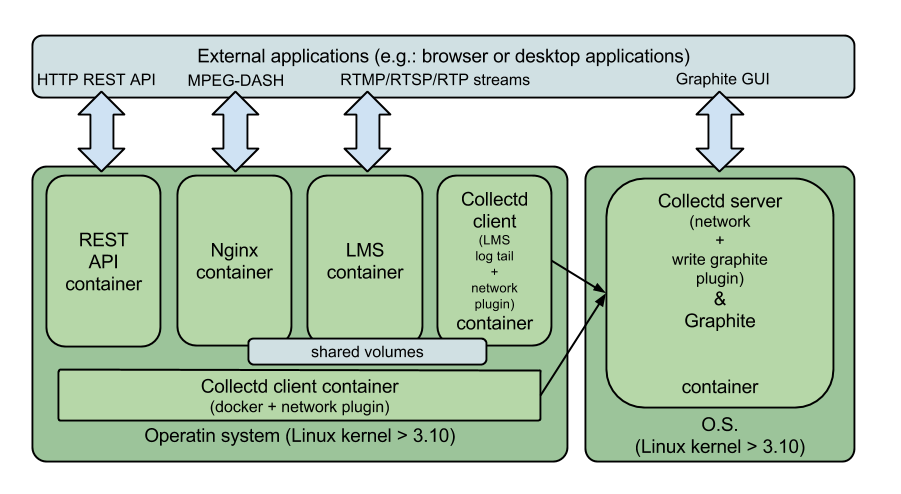
\includegraphics[width=0.9\textwidth]{./images/monitArchProp.png}
\caption{Detailed monitoring architecture}
\label{F:maex}
\end{center}
\end{figure}

Figure \ref{F:maex} showcases the relationship between different containers and the whole Collectd+Graphite deployment. Following sections are explaining it:

\section{Monitoring containers}

This section is based on how Collectd can be configured and deployed in order to monitor and properly gather metrics of interest.

\subsection{From O.S. point of view}

The fact of using Collectd means a wide community behind, which probably have already developed required functionalities (i.e.: plugins). And this is the case: in order to monitor each of the containers that a host O.S. might have it can be solved by configuring already existing plugins for Collectd from Docker community. 

The selected plugin is using the stats API introduced since Docker 1.5 version. And, concretely, the reported container's stats are:
 
\begin{itemize}
\item Network bandwidth
\item Memory usage
\item CPU usage
\item Block IO
\end{itemize}

The pluguin is called "docker-collectd-pluguin" and can be found in \href{https://github.com/lebauce/docker-collectd-plugin}{GitHub} (--REFERENCE--).

Therefore, the O.S. system requires having a basic collectd daemon running and to be configured in order to send gathered metrics to a centralized collectd server (as proposed in figure \ref{F:maex}).

So, from O.S. point of view, next example of this specific Collectd's plugins configuration showcases how to load and configure such plugins:

\begin{verbatim}

TypesDB "/usr/share/collectd/docker-collectd-plugin/dockerplugin.db"
LoadPlugin python

<Plugin python>
  ModulePath "/usr/share/collectd/docker-collectd-plugin"
  Import "dockerplugin"

  <Module dockerplugin>
    BaseURL "unix://var/run/docker.sock"
    Timeout 3
  </Module>
</Plugin>

LoadPlugin network
<Plugin network>
  Server "graphite-host-address" "graphite-host-port"
  ReportStats true
</Plugin>

\end{verbatim}

Previous Collectd configuration file sets the python (i.e.: docker-collectd-plugin) plugin as an input from the O.S. Docker API daemon and the network plugin as an output to the Collectd server.

\subsection{From container point of view}

From a container point of view and by following the premise to build containers as reusable as possible what is proposed to implement is a container that has the goal to gather the logged stats from an LMS container. This, as shown in figure \ref{F:maex}, implies sharing a Docker volume (as introduced in previous chapter \ref{D:virtualization}) from LMS container to the Collectd client which is using the tail plugin as an input. Moreover, in order to send specific logged metrics to the Collectd server container it is also using the network plugin as done in previous Collectd client configuration.

But, first of all, it is also required to be built in a container. So, this is the Docker file:

\begin{verbatim}

FROM    ubuntu:14.04
MAINTAINER Gerard CL <gerardcl@gmail.com>

ENV     DEBIAN_FRONTEND noninteractive

RUN apt-get update
RUN apt-get -y install collectd curl python-dev python-pip

ADD collectd.conf.tpl /etc/collectd/collectd.conf.tpl

RUN pip install envtpl
ADD start_container /usr/bin/start_container
RUN chmod +x /usr/bin/start_container
CMD start_container

\end{verbatim}

The, what is done in this case is to specify a bash script to run as CMD. This runs collectd but after envtpl python's package sets the environment parameters:
\begin{verbatim}
#!/bin/bash
envtpl /etc/collectd/collectd.conf.tpl
collectd -C /etc/collectd/collectd.conf -f
\end{verbatim}

Thanks to the envtpl package it is possible to run the container with specific environment variables in order to configure following parameters:

\begin{itemize}
\item LMS NAME \hfill

this will be used to identify the LMS instance in a container which Collectd is monitoring.
\item GRAPHITE HOST \hfill

this is to set the address of the remote/local container where the Collectd server is listening and pushing the metrics inside the Graphite's tools.
\item GRAPHITE PORT \hfill

this is the port where the Collect server and Graphite's tools container is listening to.
\end{itemize}

And these parameters are set in the Collectd configuration file as shown next (among the specific plugins):

\begin{verbatim}
Hostname "{{ LMS_NAME }}"
FQDNLookup true

Interval 1
Timeout 4
ReadThreads 5

LoadPlugin syslog
LoadPlugin cpu
LoadPlugin load
LoadPlugin memory
LoadPlugin network

<Plugin "syslog">
  LogLevel "info"
  NotifyLevel "OKAY"
</Plugin>

<Plugin network>
  Server "{{ GRAPHITE_HOST }}" "{{ GRAPHITE_PORT | default("25826") }}"
  ReportStats true
</Plugin>
\end{verbatim}

This Collectd configuration example file is loading specific system loggers plugins as inputs to be sent through the network plugin to the Collectd server.

But, in next chapter \ref{H:platformDeploymentAndDemonstrations} is shown an example of use of the Collectd tail plugin by using regular expressions. And this, as shown in figure \ref{F:maex}, this tail plugin is listening in an specific folder which is shared through the Docker's volume functionality with the LMS container, which logs its metrics in the same volume.

Finally, the Docker run command where the specific environment variables are set should be as shown next:
\begin{verbatim}
$ docker run -it -e "LMS_NAME=lms" \
	-e "GRAPHITE_HOST=<IP address>" -e "GRAPHITE_PORT=25826" \
	--rm --name cdc \
	-p 25826:25826/udp gerardcl/lms-collectd-client
\end{verbatim}

This will start immediately sending the defined container stats to the Graphite container specified by the environment parameters. Following section showcases the Graphite side to be deployed.

So, this example of deployed container for isolated Collectd clients is a key point in the general monitoring architecture due to the fact of being easyly configurable and reusable.

\section{Showcasing monitoring}

container amb graphite + collectd server

mostrar com es genera tot (referències a fitxers externs??) i imatges del graphite o escenari sencer. amb exemples concrets mostrant potencial de graphite!!!

This section is focused on the storage and presentation side of the metrics already logged and gathered.

So, as already introduced, this is proposed to be done within a container built with a Collectd server (network data inputs served to Graphite) and a Graphite system (storing and presenting stats).

As commonly said by the Collectd and Graphite community, installing and configuring Graphite isn't at all so easy than installing and configuring Collectd. This fact is shown in the following Docker file in order to build such container, as shown in figure \ref{F:maex}:

\begin{verbatim}
# LiveMediaStreamer Container
FROM ubuntu:14.04
MAINTAINER Gerard CL <gerardcl@gmail.com>

RUN apt-get update
RUN apt-get install -y python-cairo collectd-core libgcrypt11 \
python-virtualenv build-essential python-dev supervisor sudo

RUN adduser --system --group --no-create-home collectd \
&& adduser --system --home /opt/graphite graphite

RUN sudo -u graphite virtualenv --system-site-packages ~graphite/env

RUN echo "django \n \
  python-memcached \n \
  django-tagging \n \
  twisted \n \
  gunicorn \n \
  whisper \n \
  carbon \n \
  graphite-web" > /tmp/graphite_reqs.txt

RUN sudo -u graphite HOME=/opt/graphite /bin/sh -c ". \
~/env/bin/activate && pip install -r /tmp/graphite_reqs.txt"

ADD collectd/collectd.conf /etc/collectd/
ADD supervisor/ /etc/supervisor/conf.d/
ADD graphite/settings.py /opt/graphite/webapp/graphite/
ADD graphite/local_settings.py /opt/graphite/webapp/graphite/
ADD graphite/mkadmin.py /opt/graphite/webapp/graphite/
ADD graphite/storage-schemas.conf /opt/graphite/conf/

RUN cp /opt/graphite/conf/carbon.conf.example \
/opt/graphite/conf/carbon.conf
RUN cp /opt/graphite/conf/graphite.wsgi.example \
/opt/graphite/webapp/graphite/graphite_wsgi.py
RUN cp /opt/graphite/conf/graphite.wsgi.example \
/opt/graphite/conf/graphite.wsgi
RUN cp /opt/graphite/conf/storage-aggregation.conf.example \
/opt/graphite/conf/storage-aggregation.conf

RUN sed -i "s#^\(SECRET_KEY = \).*#\1\"`python -c 'import os; import base64; \
print(base64.b64encode(os.urandom(40)))'`\"#" \
/opt/graphite/webapp/graphite/app_settings.py
RUN sudo -u graphite HOME=/opt/graphite PYTHONPATH=/opt/graphite/lib/ \
/bin/sh -c "cd ~/webapp/graphite && ~/env/bin/python manage.py syncdb --noinput"
RUN sudo -u graphite HOME=/opt/graphite PYTHONPATH=/opt/graphite/lib/ \
/bin/sh -c "cd ~/webapp/graphite && ~/env/bin/python mkadmin.py"

EXPOSE 8080 25826/udp

CMD exec supervisord -n
\end{verbatim}

In this case, specific "collectd" and "graphite" users are created (among other environment configurations as shown).
Then, a bunch of different and specific configuration files for graphite are added (i.e.: ADD command) to their specific configuration folders. And, finally, specific command executions for database synchronization (sqlite3) and other final configurations required for Graphite are also done (--REFERENCE-- intalling graphite). Regarding Collectd, it is installed in a similiar way as previously done but it is now configured as follows:

\begin{verbatim}
Hostname "localhost"
FQDNLookup true
Interval 1

LoadPlugin syslog
LoadPlugin network
LoadPlugin write_graphite

<Plugin syslog>
	LogLevel "info"
	NotifyLevel "OKAY"
</Plugin>

<Plugin network>
	Listen "*" "25826"
	ReportStats true
</Plugin>

<Plugin write_graphite>
	<Node "graphing">
		Host "localhost"
		Port "2003"
		Protocol "tcp"
		LogSendErrors true
		Prefix "collectd."
		StoreRates true
		AlwaysAppendDS false
		EscapeCharacter "_"
	</Node>
</Plugin>
\end{verbatim}

So, here, Collectd is configured as a server by listening from anywhere at the default port for Collectd clustering. Moreover, the "write graphite" plugin is loaded in order to work as an output to the Graphite's Carbon tool, which receives the data to be stored in the Whisper RRD of the Graphite installation.

In this case, it is required to configure this container to be able to run multiple processes (i.e.: Graphite and Collectd). Therefore, by following previous section of how to run multiple processes inside a container in chapter \ref{D:virtualization}, the Supervisord system is used. This time it's configured by splitting the processes configurations into two parts, the Collectd and the Graphite. This last is configuring the Graphite web application and the Graphite's Carbon cache.

\begin{itemize}
\item Collectd: \hfill

\begin{verbatim}
[program:collectd]
user=collectd
directory=/
command=collectd -C /etc/collectd/collectd.conf -f
stdout_logfile=/var/log/supervisor/%(program_name)s.log
stderr_logfile=/var/log/supervisor/%(program_name)s_error.log
\end{verbatim}
\item Graphite web: \hfill

\begin{verbatim}
[program:graphite-web]
user=graphite
directory=/opt/graphite/webapp/
command=/opt/graphite/env/bin/gunicorn -w 1 -b 0.0.0.0:8080 \
	--pythonpath /opt/graphite/webapp/graphite graphite_wsgi
stdout_logfile=/var/log/supervisor/%(program_name)s.log
stderr_logfile=/var/log/supervisor/%(program_name)s_error.log
\end{verbatim}

\item Carbon cache: \hfill

\begin{verbatim}
[program:carbon-cache]
user=graphite
directory=/
env=PYTHONPATH=/opt/graphite/lib/
command=/opt/graphite/bin/carbon-cache.py --debug start
stdout_logfile=/var/log/supervisor/%(program_name)s.log
stderr_logfile=/var/log/supervisor/%(program_name)s_error.log
\end{verbatim}
\end{itemize}

An important configuration that must be decided and configured by knowing the requirements for why monitoring is required implies defining the storage schemas, which detail retention rates for storing metrics by following what was introduced in chapter \ref{B:problemStatementAndProposal}, the Round-Robin Database storage type. So, in order to work over a real-time media production platform it is important to achieve as much time accuracy as possible regarding the specific metrics of interest (e.g.: bandwidth usage, losses, pipeline delays, \ldots). There are more files regarding the Graphite's tools configuration (see APPENDIX XXX) too, but most of them are set to default values which are the recommended ones. 

Before going to present results and comment the outcomes (chapter \ref{H:platformDeploymentAndDemonstrations}), it is important to showcase example commands for both Collectd client and Collectd server + Graphite's containers:

\begin{verbatim}
$ docker run -it -e "LMS_NAME=lms" -e "GRAPHITE_HOST=<IP of >" \
--rm --name collectd -p 25826:25826/udp gerardcl/lms-collectd-client
\end{verbatim}

\begin{verbatim}
$ docker run -it --rm --name graphite -p 25826:25826/udp -p 8080:8080 \
gerardcl/lms-collectd-graphite
\end{verbatim}

As shown, the collectd (i.e.: Collectd client) container is sending to the default port (i.e.: UDP protocol) of the graphite host's (Collectd server and Graphite tools) container. Moreover, the graphite container opens HTTP port 8080 in order to enable browsers to get access to its web application anywhere. 

\chapter{Platform deployment tests, and results}\label{H:platformDeploymentAndDemonstrations}

In order to demonstrate that the LiveMediaStreamer is a suitable tool to be used as the core framework of a cloud real-time media production platform it is required to test how it performs over the cloud.

\section{Platform deployment}

In order to demonstrate how LMS fits the project requirements two scenarios, with different complexity, are deployed.

\begin{itemize}
\item Isolated deployments \hfill

The main goal of this deployment is to demonstrate how LMS performs inside a Docker container by comparing its performance in the same OS but without running inside a container (i.e.: system installation).

In this scenario LMS is configured to act as a transcoder service. This means applying one pipeline per stream type (i.e.: one video and one audio paths).

\item Generic deployment scenario \hfill

This scenario aims to showcase a suitable and as much generic as possible cloud real-time media production scenario. LMS is configured to receive eight streams (i.e.: four audio and four video streams), mix them and transmit them through RTP/RTSP. 
\end{itemize}

The environment where the deployments are done is composed of two laptops. The LMS container and the Collectd client container are deployed in laptop described in Table \ref{T:dec}. The second laptop is a Dual-Core PC with the Graphite container running. Note that the first laptop described has the highest computational cost because all the audio and video processing is done in. The second laptop only stores the statistics, displays the Graphite graphs in a browser, plays the LMS's output streams and transmits a video source (2 Mbps H.264 encoded video stream at 25 fps and at 1280x720 pixels resolution) as input for the LMS.

\begin{table}[htb]
\caption{Deployment environment characteristics}
\begin{center}
\begin{tabular}{|c|c|}
\hline
{\bf Parameter} & {\bf Value} \\ \hline \hline
Hardware type        & Sony VAIO laptop \\ \hline
CPU        & Intel core i7-3632QM at 2.20 GHz  \\ \hline
RAM        & 6 GB (4 + 2) DDR3 \\ \hline
Operating system        & XUbuntu 14.04 - 64 bits (x86 64)  \\ \hline
Kernel version        & 3.13.0-55-generic  \\ \hline
Docker version        & 1.6.8  \\ \hline
\end{tabular}
\label{T:dec}
\end{center}
\end{table}

As seen, the deployment has not been carried out in any type of specific server or high performance cluster environment. The main goal is to demonstrate flexibility on the deployment (i.e.: in a laptop) and portability of the platform (not only the cloud itself). All of these characteristics are achieved thanks to the performance of the platform itself and the LMS (the core).

Note that all tests have been carried out in a 1 Gbps local area network with a router with both laptops connected (see Figure \ref{F:idsc} and Figure \ref{F:gdsc}). The measurements have been carried out during 10 minutes and a second of granularity.

\subsection{Isolated deployments}

This section compares the performance of the LMS installed on system (i.e.: in the host OS) and the same LMS inside a container. A C/C++ script has been developed, which configures the LMS framework as shown in Figure \ref{F:idsc}. Moreover, in order to test the performance, the pipeline metrics are logged once per second (i.e.: pipeline losses and delay) and gathered by a Collectd client container properly configured. Then the Collectd client sends the data to the Graphite container. Check Appendix \ref{ANX:dockerFiles} section \ref{ANX:collectdTailFiles2} to see an example of how the logging and collecting is implemented for these demonstrations. 

\begin{figure}[!htb]
\begin{center}
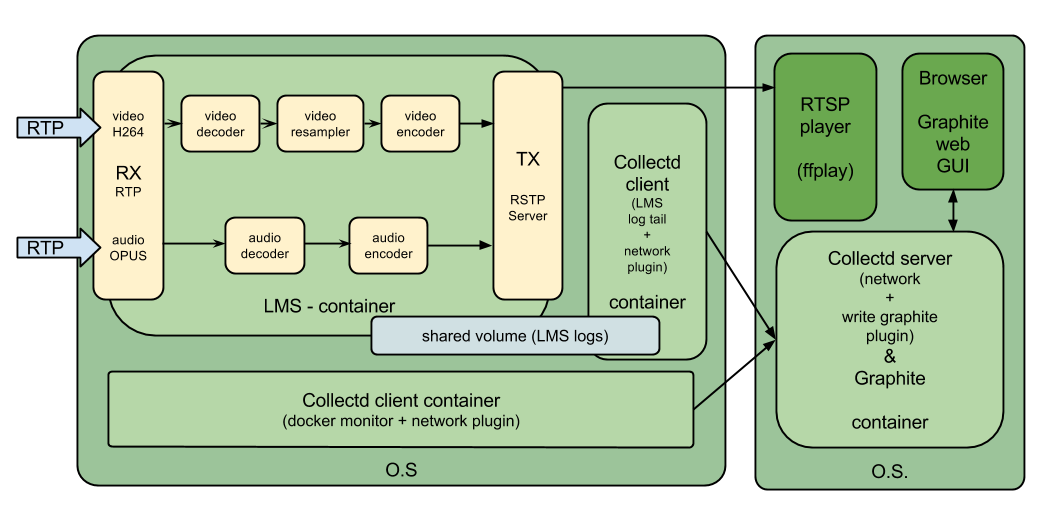
\includegraphics[width=0.95\textwidth]{./images/isolatedScenario.png}
\caption{Configuration of the scenario for the isolated deployments}
\label{F:idsc}
\end{center}
\end{figure}

The Collectd client container, which reads from the folder where the LMS is logging its metrics, uses the \texttt{tail} plugin (previously explained in Chapter \ref{G:monitoringLayer}) with specific regular expressions in order to parse the metrics from the LMS logs.

Both isolated scenarios are the same but one is running the LMS on the system and the other is running the same configured LMS but containerized. The second OS is the one which runs the Docker container with the Collectd+Graphite tools. Moreover, this OS acts as the receiver of the transcoded streams through the RTSP protocol and also acts as the transmitter of the source stream.

Figure \ref{F:isoCPU} shows the results. These are mainly focused on the pipeline performance metrics (i.e.: internal LMS performance). The figure describes the CPU usage gathered at the Collectd client side and presented for the Graphite web GUI for both isolated scenarios. Regarding system installation the CPU average usage of the averages given by Graphite is around 4,015\% and around 4,111\% for the containerized one. So, there is not so difference about running system installation or the same application containerized.

\begin{figure}[!htb]
  \begin{center}
    \begin{subfigmatrix}{2}
      \subfigure[System installation]
         {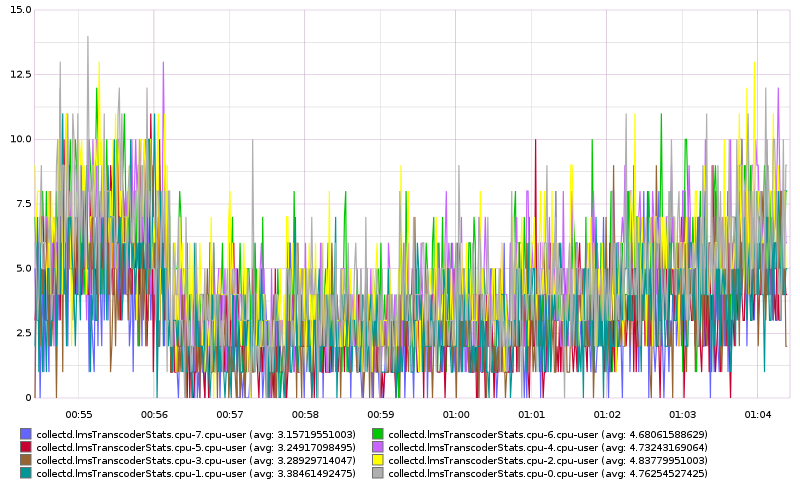
\includegraphics{./images/testStats/testStatsOS/8cpuIdleAVG.png}\label{SF:S1}} 
      \subfigure[Containerized]
         {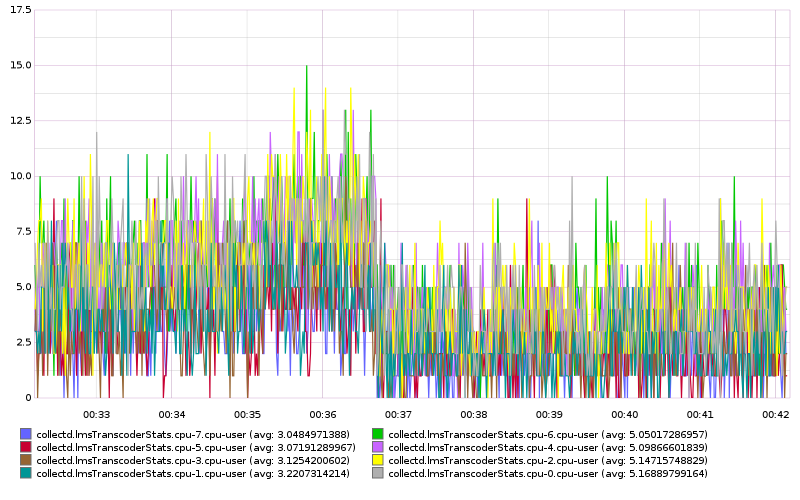
\includegraphics{./images/testStats/testStatsDocker/8cpuIdleAVG.png}\label{SF:S2}} 
    \end{subfigmatrix}
    \caption{Isolated scenarios - CPU usage}
    \label{F:isoCPU}
  \end{center}
\end{figure}

Figure \ref{F:isoappt} illustrates the average pipeline delay introduced by the LMS system, which in both video and audio cases is almost the same. Regarding video, system installation reaches an average of 216,8 milliseconds and the containerized case reaches an average of 215,9 milliseconds. Regarding audio, system installation reaches an average of 25,6 milliseconds and the containerized reaches an average of 25,2 milliseconds.

\begin{figure}[!htb]
  \begin{center}
    \begin{subfigmatrix}{2}
      \subfigure[System installation - Video path]
         {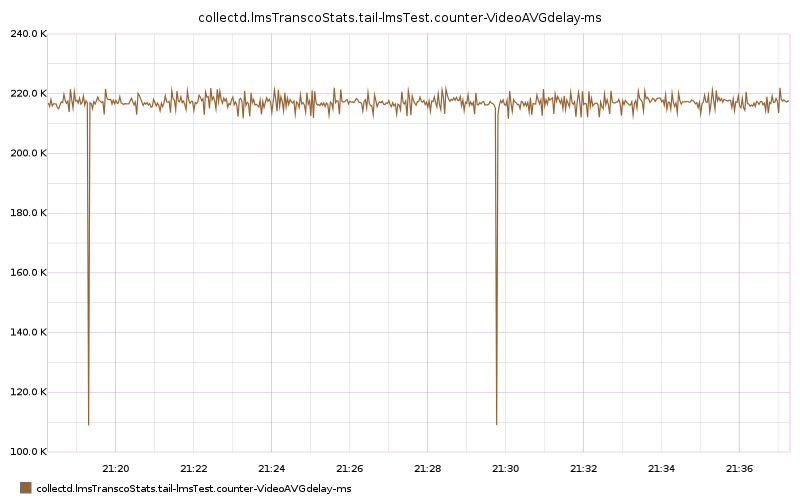
\includegraphics{./images/testStats/testStatsOS/vAVGdelayMS.png}\label{SF:S3}} 
      \subfigure[Containerized - Video path]
         {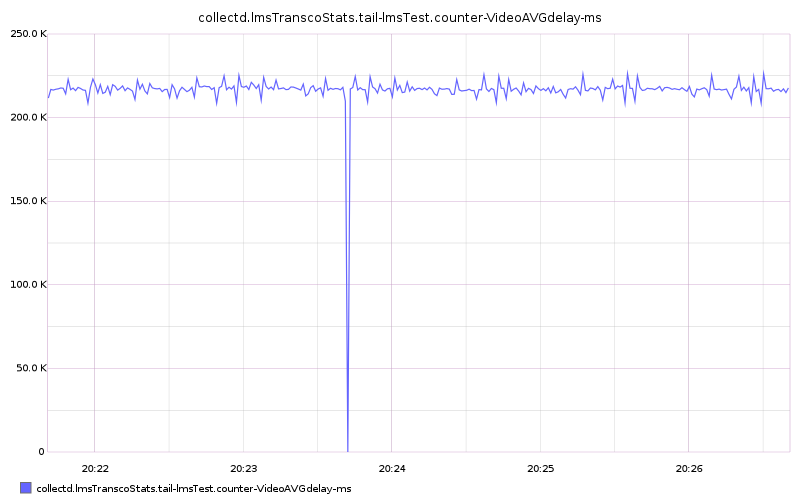
\includegraphics{./images/testStats/testStatsDocker/vAVGdelayMS.png}\label{SF:S4}} 
      \subfigure[System installation - Audio path]
         {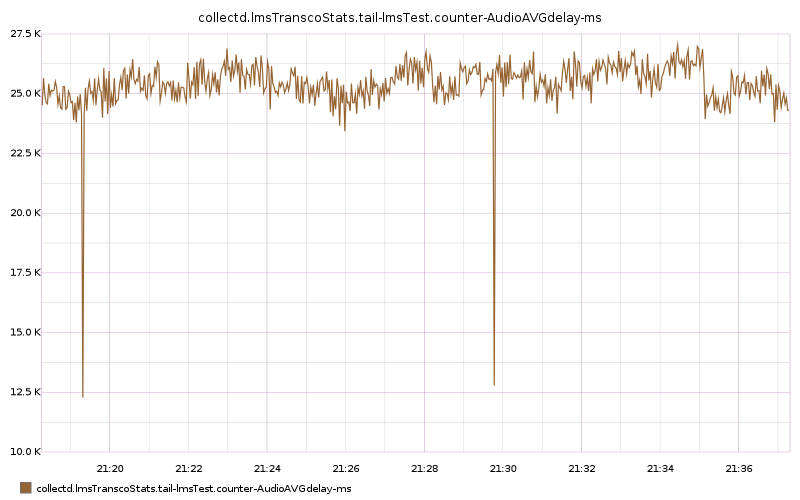
\includegraphics{./images/testStats/testStatsOS/aAVGdelayMS.png}\label{SF:S3}} 
      \subfigure[Containerized - Audio path]
         {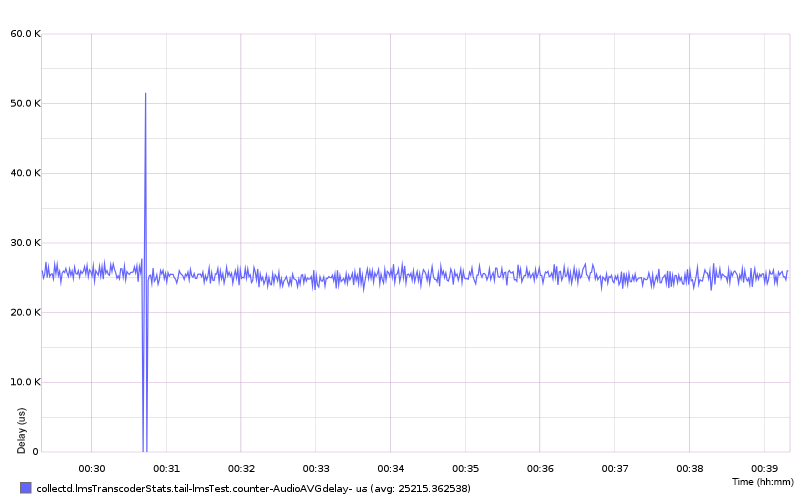
\includegraphics{./images/testStats/testStatsDocker/aAVGdelayMS.png}\label{SF:S4}}
    \end{subfigmatrix}
    \caption{Isolated scenarios - average pipeline processing time}
    \label{F:isoappt}
  \end{center}
\end{figure}



\begin{figure}[!htb]
  \begin{center}
    \begin{subfigmatrix}{2}
      \subfigure[System installation - Video path]
         {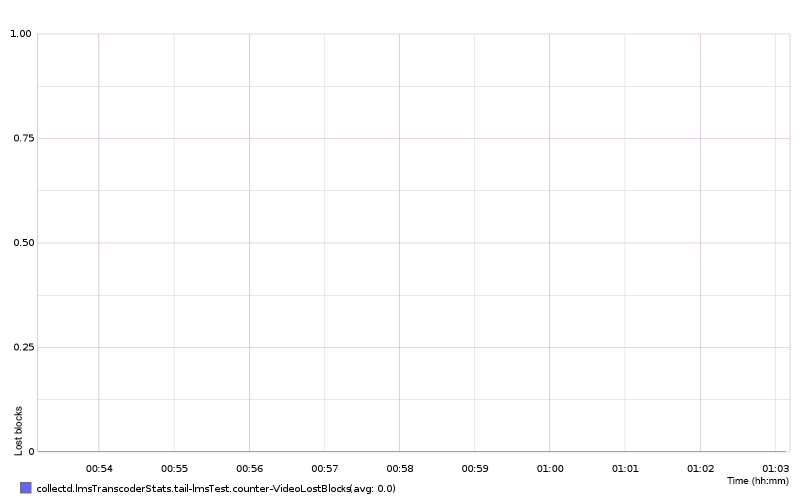
\includegraphics{./images/testStats/testStatsOS/vLostBlocs.png}\label{SF:S3}} 
      \subfigure[Containerized - Video path]
         {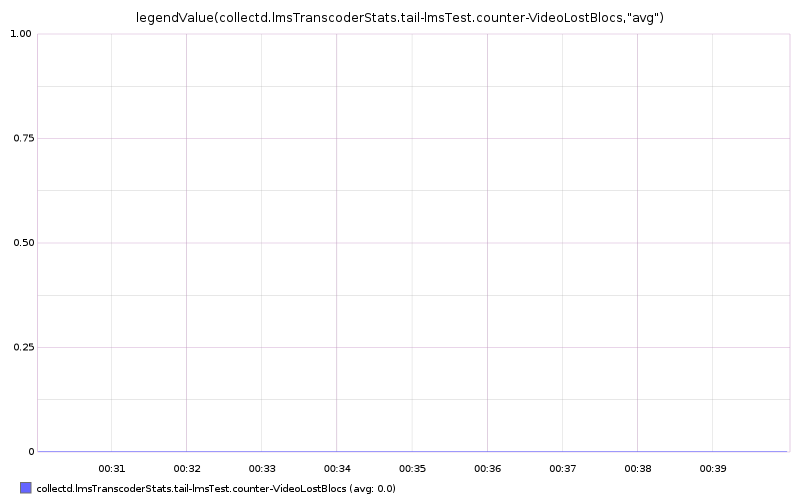
\includegraphics{./images/testStats/testStatsDocker/vLostBlocs.png}\label{SF:S4}} 
      \subfigure[System installation - Audio path]
         {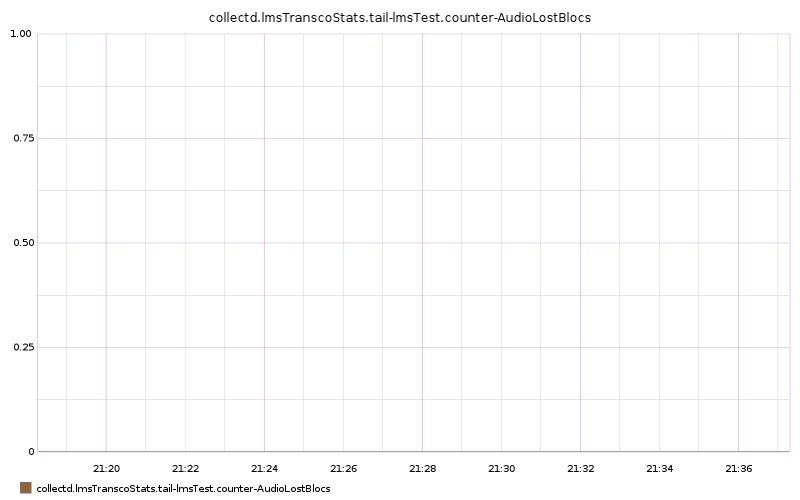
\includegraphics{./images/testStats/testStatsOS/aLostBlocs.png}\label{SF:S3}} 
      \subfigure[Containerized - Audio path]
         {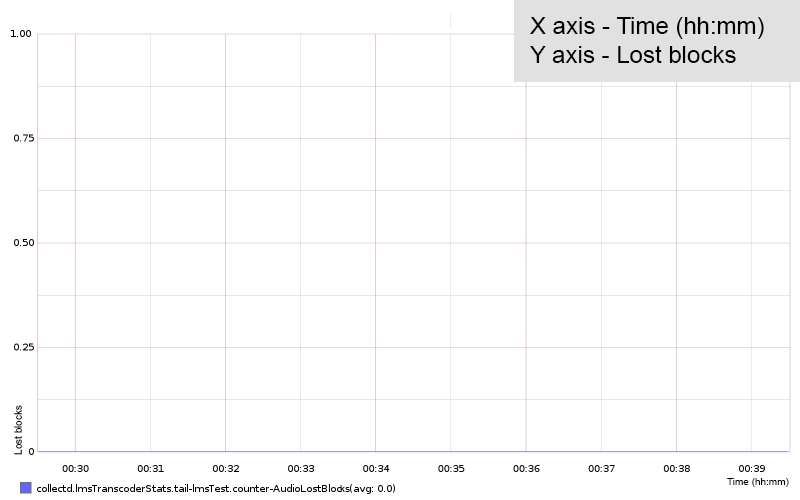
\includegraphics{./images/testStats/testStatsDocker/aLostBlocs.png}\label{SF:S4}}
    \end{subfigmatrix}
    \caption{Isolated scenarios - pipeline accumulated lost blocks}
    \label{F:isoaplb}
  \end{center}
\end{figure} 

\vbox{Regarding pipeline losses, as shown in Figure \ref{F:isoaplb}, both pipelines within both system installation and containerized scenarios do not introduce any data loss. Therefore, LMS is a good option to work with, not only on system installation but also in a containerized environment in order to be a portable service over a cloud infrastructure.}

\subsection{Generic scenario deployment}

This last scenario is a generic and basic example demonstration of audio and video production in a cloud environment. Figure \ref{F:gdsc} illustrates how the scenario is configured.

\begin{figure}[htb]
\begin{center}
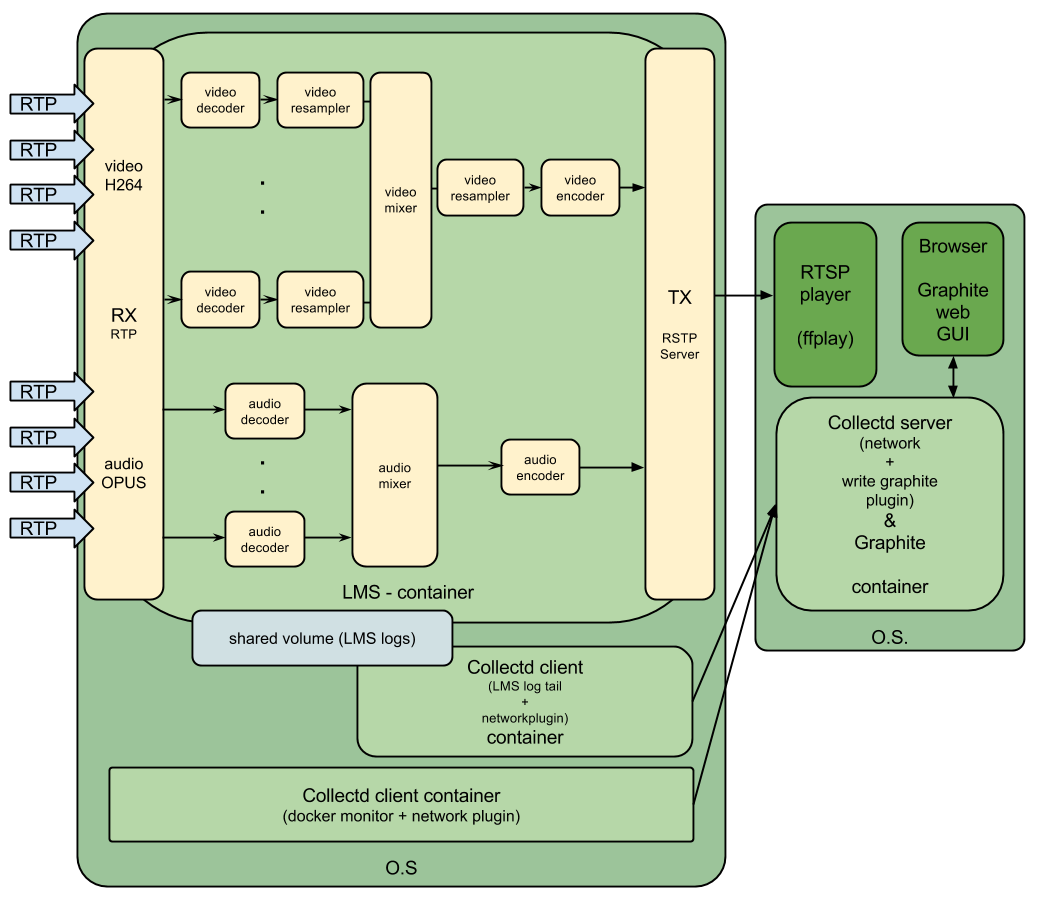
\includegraphics[width=0.95\textwidth]{./images/genericScenario.png}
\caption{Configuration of the scenario for the generic deployment}
\label{F:gdsc}
\end{center}
\end{figure}

This demonstration is quite similar to the previous but this time LMS is only configured and running inside a container. This LMS configuration is also a C/C++ script which configures the framework, as shown in Figure \ref{F:gdsc}, inside the LMS container, specifically.

In this case what is deployed is an audio and video mixer which receives four audio streams and four video streams encoded with OPUS and H264 codecs, respectively, which are streamed through its standard RTP encapsulation (i.e.: specific payload headers).

Regarding the audio mixing, all input streams are mixed using the logarithmic mixing algorithm in order to not saturate the signal of the resulting audio stream. Regarding the video mixing, the HD inputs (at 1280x720 pixels resolution) are mixed as shown in Figure \ref{F:outVMix}. All video inputs are resized (through the pre-resampler filter to the video mixer, see Figure \ref{F:gdsc}) to half of its size in order to fit into a resulting HD video stream as shown in Figure \ref{F:gdsc}.

\begin{figure}[!htb]
\begin{center}
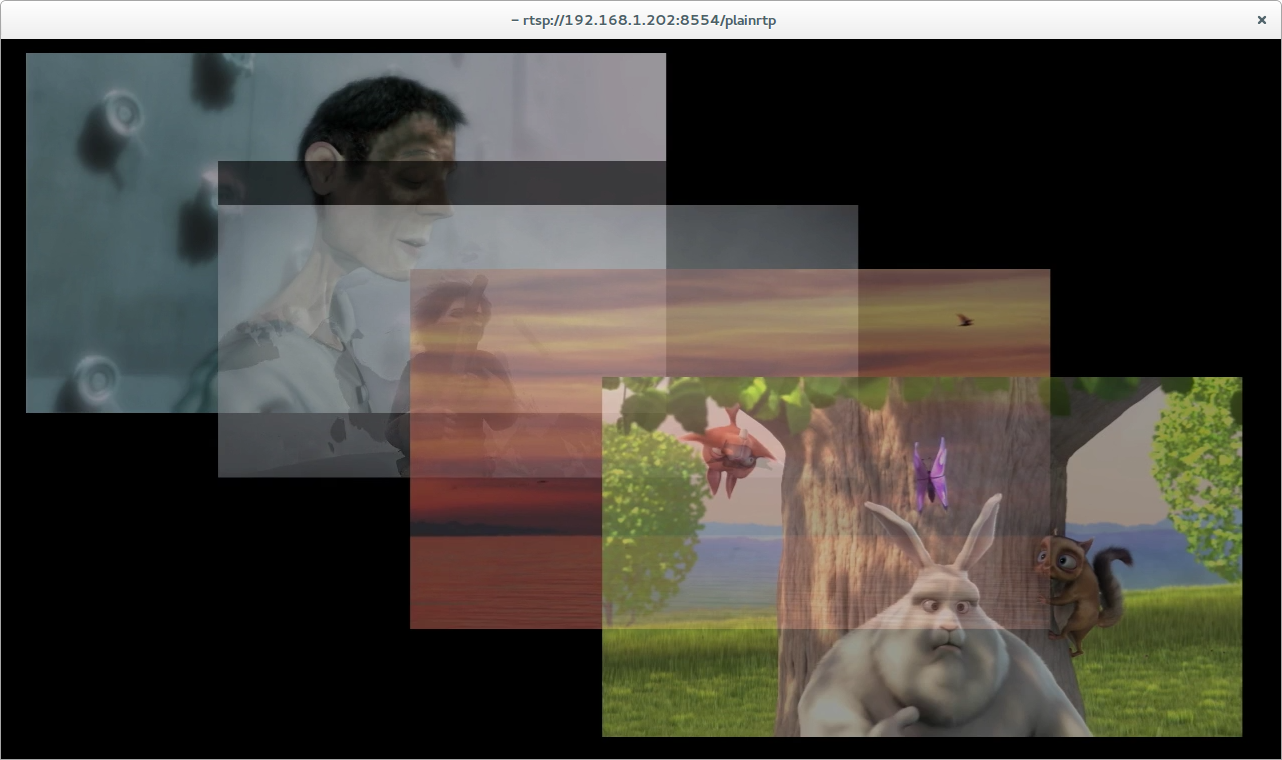
\includegraphics[width=0.90\textwidth]{./images/outAVmix.png}
\caption{Generic scenario - video mixing configuration result}
\label{F:outVMix}
\end{center}
\end{figure}

\vbox{Let us focus now on the results regarding the pipeline performance parameters. The CPU usage of the containerized audio and video mixer obtained by averaging the averages, shown in Figure \ref{F:gsavgcpu}, is 23,02\%.}

\begin{figure}[!htb]
\begin{center}
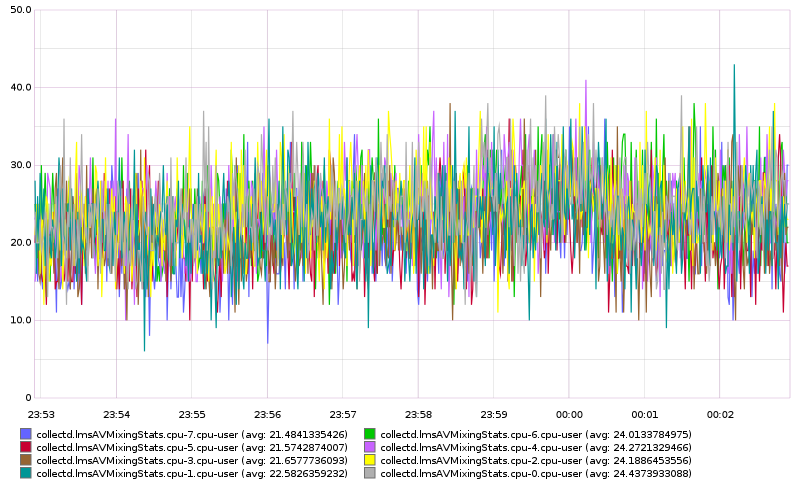
\includegraphics[width=0.90\textwidth]{./images/testAVMix/AVMixCPU.png}
\caption{Generic scenario - average CPU usage}
\label{F:gsavgcpu}
\end{center}
\end{figure}

\vbox{The audio and video average pipeline delay introduced in this scenario is shown in Figure \ref{F:gsavgpt}. There are two path groups, the "recevier to mixer" paths and the "mixer to transmitter" path (see Figure \ref{F:gdsc}).}

\begin{figure}[!htb]
  \begin{center}
    \begin{subfigmatrix}{2}
      \subfigure[Audio paths]
         {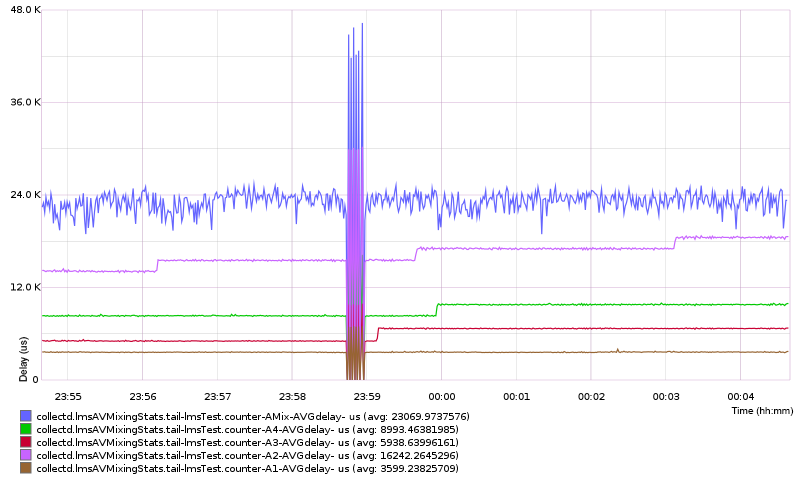
\includegraphics{./images/testAVMix/AVMixAudioAVGdelay.png}\label{SF:S5}} 
      \subfigure[Video paths]
         {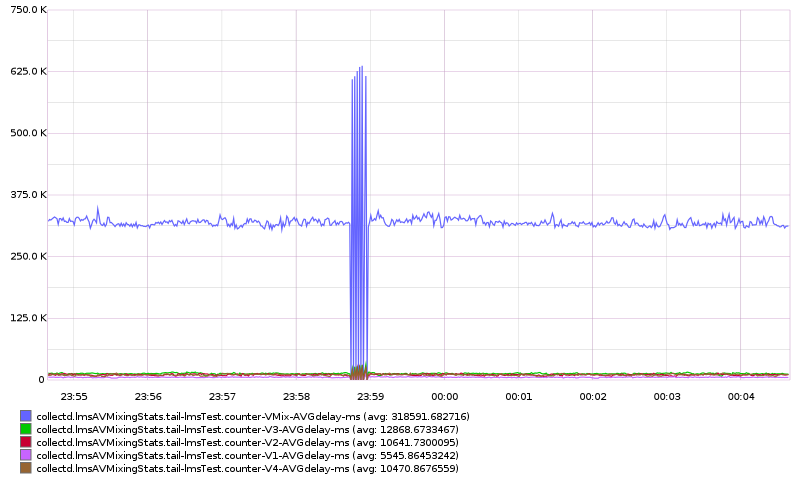
\includegraphics{./images/testAVMix/AVMixVideoAVGdelay.png}\label{SF:S6}} 
    \end{subfigmatrix}
    \caption{Generic scenario - paths average processing time}
    \label{F:gsavgpt}
  \end{center}
\end{figure}

\vbox{The average delay introduced for the audio "receiver to mixer" paths averages is 8,6 milliseconds and the audio "mixer to transmitter" path average delay is 23,1 milliseconds. Then, by adding the maximum average path (16,2 ms), a total average value of 39,3 milliseconds of processing time involving the audio pipeline is achieved. Regarding the pipeline's video path, an average of 9,89 milliseconds is obtained by averaging the "receiver to mixer" video paths average processing times. By adding the average of the "mixer to transmitter" path processing time of 67 milliseconds to the maximum average obtained in the "receiver to mixer" path (12,8 ms) a total average of 79,8 milliseconds of delay introduced for the video pipeline is obtained. Therefore, the generic scenario demonstrates that LMS achieves acceptable processing time values for real-time\footnote{Real-time parameters, in media streaming, mean a total processing time (i.e.: added delay between origin and destination) of 150 to 200 milliseconds} audio-visual media content production.}

\begin{figure}[!htb]
  \begin{center}
    \begin{subfigmatrix}{2}
      \subfigure[Audio paths]
         {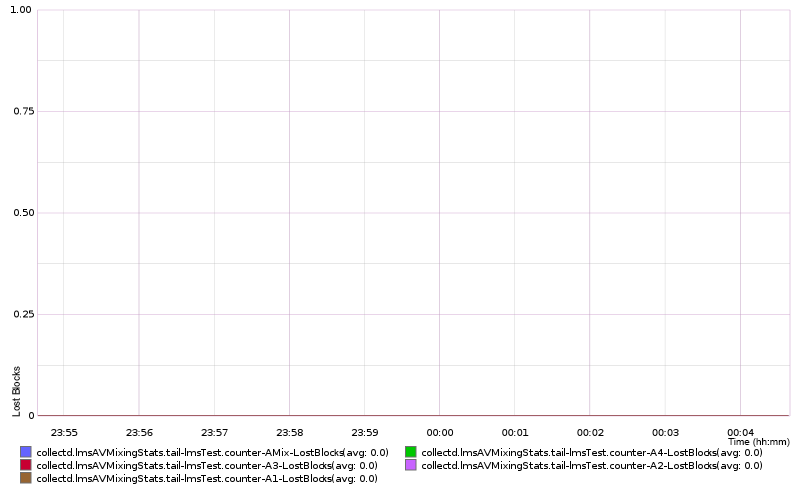
\includegraphics{./images/testAVMix/AVMixAudioLostBlocs.png}\label{SF:S7}} 
      \subfigure[Video paths]
         {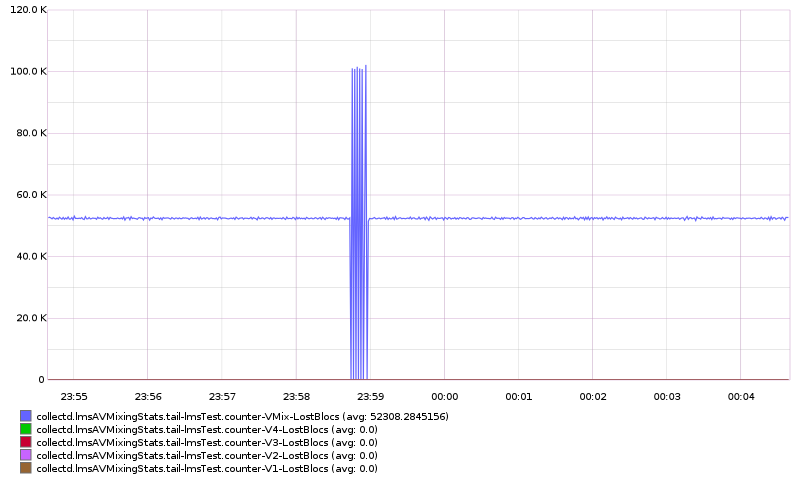
\includegraphics{./images/testAVMix/AVMixVideoLostBlocs.png}\label{SF:S8}} 
    \end{subfigmatrix}
    \caption{Generic scenario - paths accumulated lost blocks}
    \label{F:gsalb}
  \end{center}
\end{figure}

\vbox{Figure \ref{SF:S7} illustrates that the audio paths of the accumulated lost blocks remains to zero, meaning that the audio pipeline is not discarding any data at any filter, which is an important fact because losing any byte of audio would mean noticing some effects (i.e.: audio clips).} 

Then regarding the video "receiver to mixer" paths there aren't accumulated data losses. But, "mixer to transmitter" path reaches around 52.308 lost data blocks. The fact of having lost data blocks is due to the transitory period of the mixer filter. However, this accumulated losses remains constant, meaning that there are no more data blocks lost.

So, although this scenario is being deployed in a i7 processor laptop, it's able to real-time mix four couples of audio and video streams without issues.

Finally, to point out that the signal discontinuities that appear in some figures are due to the fact of transmitting origin streams in a pseudo-live mode, which means audio and video loops. Therefore, this noise appears when the origin streams restart.
\cleardoublepage
\phantomsection
\chapter*{Conclusions}

Escriure aquí les conclusions del projecte. 

LINKS CONCLUSIONS

http://windowsitpro.com/blog/going-beyond-virtualization-private-cloud

vGPU

virtualization and monitoring are the key start points to develop a ...
\cleardoublepage
\phantomsection
\chapter*{Acronyms}

\begin{table*}[htb]
\centering
\begin{tabular}{p{0.2\textwidth} p{0.7\textwidth}}
\hline
OTT & Over The Top \\
\hline
SDN & Software Defined Networks \\
\hline
RTP & Real-time Transport Protocol \\
\hline
\end{tabular}
\end{table*}




%\chapter{Organització del treball}

\section{Pàgines preliminars}

\subsection{Portada}\label{S:portada}

No cal triar cap altre document per la portada. En funció de com hàgiu configurat el fitxer \texttt{dades.tex} la portada es generarà automàticament. Un altre avantatge d'aquesta plantilla \LaTeX \ :-)

\subsection{Resum}

\subsubsection{Identificador del treball/projecte}

Cal fer la identificació del treball/projecte de la mateixa manera que consta en la portada (apartat \ref{S:portada})

\subsubsection{Resum}

El Resum del treball ha de ser autocontingut i ha de presentar de manera concisa els objectius, la metodologia utilitzada i els resultats obtinguts. No és aconsellable incloure-hi referències numèriques. Tal i com queda recollit a la normativa s'ha de presentar un resum en català/castellà i un altre en anglès. El resum ha de tenir una extensió mínima de 1500 caràcters sense espais i una extensió màxima de 3000.


\subsection{Dedicatòria}

En el cas que es vulgui dedicar el treball/projecte a algú, cal afegir-hi la dedicatòria en un full apart, després del resum i abans de l'índex. L'entorn \texttt{dedicatoria} proporcionat amb aquesta plantilla ja formata la dedicatoria adientment. 


\subsection{Índex}

Pel que fa a l'índex, no cal fer absolutament res. Aquesta plantilla \LaTeX \ ja el fa tot per vosaltres :-)

D'altra banda pot ser molt recomanable afegir en el full següent un Índex de figures i taules per facilitar-ne la localització. La confecció d'aquest índex també és automàtica i  \LaTeX \ ja ho fa tot per vosaltres :-)

  
\section{Cos del treball}

\subsection{Introducció}

A la Introducció cal explicar la finalitat del treball i els mètodes utilitzats, així com les principals conclusions a què s'hagi arribat. Es pot considerar una versió ampliada del resum.

També cal explicitar a la introducció la justificació de la divisió del treball en capítols, atès que aquesta no pot ser una divisió qualsevol del treball, sinó que ha de seguir un ordre lògic.

Així mateix, és necessari incloure-hi els termes clau del treball amb la seva definició correcta, i aquelles abreviatures i fórmules bàsiques imprescindibles per a la comprensió del text.

És molt important que la introducció no sigui molt extensa perquè el lector pugui fer-hi una ullada ràpida i entendre'n el contingut o fer-ne memòria en qualsevol moment.


\subsection{Confecció dels capítols}

Des del punt de vista de la comprensió i de l'estètica, és aconsellable que els capítols tinguin més o menys la mateixa extensió. Els capítols més llargs es poden dividir en seccions o reduir-los i incloure alguns detalls als apèndixs.


\subsection{Fórmules, figures i taules}

\subsubsection{Fórmules}

Pel que fa al format de les formules, no cal fer absolutament res. \LaTeX \ ja ho fa tot per vosaltres :-)  

Simplement el que heu de fer és escriure la fórmula com per exemple:

\begin{equation}\label{E:prova}
\sum _{i=0}^{N} \sum _{j=0}^{N} \frac{\lambda _{ij}}{\alpha _i \beta_ j} \cdot \cos (2\pi f_i) \sin(2 \pi f_j)
\end{equation}

i per citar-la és tant fàcil com fer: \ref{E:prova}

\subsubsection{Figures}

Pel que fa al format de les figures, no cal fer absolutament res. \LaTeX \ ja ho fa tot per vosaltres :-) . 

Simplement el que heu de fer és inserir la figura amb el codi següent:

\begin{verbatim}
\begin{figure}[htb]
\begin{center}

\includegraphics[width=0.5\textwidth]{./setup/EETAC-positiu-negre}
\caption{Exemple de figura}
\label{F:prova}
\end{center}
\end{figure}
\end{verbatim}

donant com a resultat la figura \ref{F:prova}.

\begin{figure}[htb]
\begin{center}

\includegraphics[width=0.5\textwidth]{./setup/EETAC-positiu-negre}
\caption{Exemple de figura}
\label{F:prova}
\end{center}
\end{figure}

Podem tocar la variable \texttt{width} per ajustar l'amplada de la figura com més ens convingui. Teniu en compte que la variable \texttt{textwidth} guarda el valor de l'amplada del texte dins la pàgina i per tant és una bona referència per delimitar amplades de figura, així doncs, la figura \ref{F:prova} ocupa la meitat de l'amplada del texte en una pàgina. 

Podeu arranjar múltiples imatges en una sola figura amb el paquet \texttt{subfigmat}, que defineix un nou entorn \texttt{subfigmatrix} que accepta per argument el nombre de columnes del arranjament. Per exemple, per fer una figura amb tres columnes d'imatges:

\begin{verbatim}
\begin{figure}[htb]
  \begin{center}
    \begin{subfigmatrix}{3}
      \subfigure[Títol subfigura 1]
         {
\includegraphics{./setup/EETAC-positiu-negre}\label{SF:S1}} 
      \subfigure[Títol subfigura 2]
         {
\includegraphics{./setup/EETAC-positiu-negre}\label{SF:S2}} 
      \subfigure[Títol subfigura 3]
         {
\includegraphics{./setup/EETAC-positiu-negre}\label{SF:S3}} 
      \subfigure[Títol subfigura 4]
         {
\includegraphics{./setup/EETAC-positiu-negre}\label{SF:S4}} 
      \subfigure[Títol subfigura 5]
         {
\includegraphics{./setup/EETAC-positiu-negre}\label{SF:S5}} 
      \subfigure[Títol subfigura 6]
         {
\includegraphics{./setup/EETAC-positiu-negre}\label{SF:S6}} 
    \end{subfigmatrix}
    \caption{Exemple d'arranjament amb múltiples imatges}
    \label{F:prova2}
  \end{center}
\end{figure}
\end{verbatim}

que dona com a resultat, la figura \ref{F:prova2}.

\begin{figure}[htb]
  \begin{center}
    \begin{subfigmatrix}{3}
      \subfigure[Títol subfigura 1]{
\includegraphics{./setup/EETAC-positiu-negre}\label{SF:S1}} 
      \subfigure[Títol subfigura 2]{
\includegraphics{./setup/EETAC-positiu-negre}\label{SF:S2}} 
      \subfigure[Títol subfigura 3]{
\includegraphics{./setup/EETAC-positiu-negre}\label{SF:S3}} 
      \subfigure[Títol subfigura 4]{
\includegraphics{./setup/EETAC-positiu-negre}\label{SF:S4}} 
      \subfigure[Títol subfigura 5]{
\includegraphics{./setup/EETAC-positiu-negre}\label{SF:S5}} 
      \subfigure[Títol subfigura 6]{
\includegraphics{./setup/EETAC-positiu-negre}\label{SF:S6}} 
    \end{subfigmatrix}
    \caption{Exemple d'arranjament amb múltiples imatges}
    \label{F:prova2}
  \end{center}
\end{figure}

%%%%%%%%%%%%%%%%%%%%%%%%%%%%%%%%%%%%%%%%%%%%%%%%%%%%%%%%%%%%%%%%%%%%%%%%%%%%%%


\subsubsection{Taules}

Pel que fa a la numeració de les taules, no cal fer gran cosa. \LaTeX \ ja fa gran part de la feina bruta. 

Simplement el que heu de fer és inserir la figura amb el codi següent:

\begin{verbatim}
\begin{table}[htb]
\begin{center}
\begin{tabular}{|c|l|r|}
\hline
{\bf Títol de la Columna 1} & {\bf Títol de la Columna 2} & 
{\bf Títol de la Columna 3}  \\ \hline \hline
centrada        & a l'esquerra    & a la dreta       \\ \hline
centrada        & a l'esquerra    & a la dreta       \\ \hline
centrada        & a l'esquerra    & a la dreta       \\ \hline
centrada        & a l'esquerra    & a la dreta       \\ \hline
centrada        & a l'esquerra    & a la dreta       \\ \hline
\end{tabular}
\caption{Exemple de taula}
\label{T:prova}
\end{center}
\end{table}
\end{verbatim}

donant com a resultat la taula \ref{T:prova}.


\begin{table}[htb]
\caption{Exemple de taula}
\begin{center}
\begin{tabular}{|c|l|r|}
\hline
{\bf Títol de la Columna 1} & {\bf Títol de la Columna 2} & {\bf Títol de la Columna 3}  \\ \hline \hline
centrada        & a l'esquerra    & a la dreta       \\ \hline
centrada        & a l'esquerra    & a la dreta       \\ \hline
centrada        & a l'esquerra    & a la dreta       \\ \hline
centrada        & a l'esquerra    & a la dreta       \\ \hline
centrada        & a l'esquerra    & a la dreta       \\ \hline
\end{tabular}
\label{T:prova}
\end{center}
\end{table}

L'entorn \texttt{tabular} que ofereix \LaTeX \ és molt complet i permet crear multitud de taules diferents, tot i que és alhora bastant complexe. Cau fora de les intencions del present document descriure la sintaxis i el format d'aquest tipus d'entorn. És molt fàcil trobar informació al respecte amb llibres especialitzats o simplement a Internet. 


\subsection{Estudi d'ambientalització}

En general l'estudi d'ambientalització es podrà incloure dins de la introducció o a les conclusions, llevat del cas que les repercussions ambientals del treball tinguin una importància tant rellevant que sigui recomanable dedicar-hi un capítol específic.


\subsection{Bibliografia}

Tret que el treball consisteixi en la cerca de bibliografia sobre un tema concret, la bibliografia ha de contenir només la llista d'obres consultades.

A la bibliografia s'han de llistar conjuntament llibres i articles de revistes. Citar una referència bibliogràfica és tant fàcil com fer:

\begin{verbatim}
\cite{prova1}
\end{verbatim}

per citar la referència \cite{prova1}.

El format de la bibliografia es genera automàticament. Un altre (gran!) avantatge del \LaTeX \ :-)


\section{Apèndixs}

En general, cal posar als apèndixs totes les dades i documents que farien el text feixuc i dificultarien la seva lectura, sense oblidar que les contínues referències als apèndixs poden obligar al lector a interrompre constantment la lectura del treball. És per això, que els apèndixs poden incloure diagrames, dades estadístiques, taules de resultats i desenvolupaments teòrics complementaris.

En el cas que, amb el conjunt d'apèndixs, el treball tingui una extensió superior als 100 fulls (aproximadament 200 pàgines), els apèndixs s'han de enquadernar en un volum separat del cos principal del treball. Aquesta plantilla ja proporciona les eines necessàries per fer la portada necessària en cas d'enquadernar els apèndixs per separat.




%%%  BIBLIOGRAFIA
%%%%%%%%%%%%%%%%%%%%%%%%%%%%%%%%%%%%%%%%%%%%%%%%%%%%%%%%%%%%%%%%%%%%%%%%%%

%%% Per la bibliografia hi ha 2 opcions: generarla amb la utilitat BibTeX 
%%%                                      o fer-la ''a ma''
%%% NOTA: podeu trobar facilment informació sobre BibTeX a:
%%%  http://www.ctan.org/tex-archive/biblio/bibtex/contrib/doc/

%%% OPCIO 1: BibTeX (recomanat) -> descomentar les comandes seguents:
%\bibliographystyle{unsrt}   %% Estil de bibliografia EETAC
%\cleardoublepage
%\phantomsection
% Indicar aqui el(s) fitxer(s) que contenen la bibliografia
%\bibliography{fitxer1,...,fitxerN}  
%\pdfbookmark{Bibliografia}{sec:biblio}

%%% OPCIO 2: bibliografia manual
%%%
%%% L'argument d'entrada es el numero de referencies que s'inclouen
\cleardoublepage
\phantomsection
\begin{thebibliography}{2}

%% Llibres:  Autor/s (cognoms i inicials dels noms), títol del llibre (en cursiva), editor, ciutat i any de publicació. Quan es cita el capítol d'un llibre s'ha d'indicar el títol del capítol (entre cometes), el títol del llibre (en cursiva) i els números de pàgines amb la primera i la darrera incloses.

%%  Exemple de capitol en llibre
%\bibitem{example} 
%Ortiz Ramirez, A.
%``Three-Tier Architecture''. {\it Títol del llibre}.
%(Editor. Ciutat. Any publicació): pagina1--paginaN.

\bibitem{ottVSiptv} 
Narang, N.
``Concept Series : What is the Difference between OTT and IPTV''. {\it M\&E Industry Trends, Technology and Research}.
1--1. (2013) 

%%  Exemple de d'article en revista
\bibitem{n-tier architecture} 
Ortiz Ramirez, A.
``Three-Tier Architecture''. {\it Linux Journal}.
{\bf volum}(75),
1--1. (2000) 

\bibitem{i2catua}
i2CAT Foundation - Audiovisual Unit. Homesite: \url{http://i2cat.net/en/area/audiovisual}

\bibitem{lmsGITHUB}
LiveMediaStreamer framework project. Homesite: \url{https://github.com/ua-i2cat/liveMediaStreamer}

\bibitem{osi} 
Zimmermann , H.
``OSI Reference Model - The ISO Model of Architecture for Open Systems Interconnection''. {\it IEEE TRANSACTIONS ON COMMUNICATIONS}.
{\bf volum}(28 - 4),
425--432. (1980) 

\bibitem{smpte}
Society of Motion Picture \& Television Engineers. Homesite: \url{https://www.smpte.org/standards}

\bibitem{SDI} 
Poynton, Charles A.
``Digital Video Interfaces''. {\it Digital Video and HDTV: Algorithms and Interfaces}.
(Morgan Kaufmann. San Francisco. 2003): 130--131.

\bibitem{3GSDI}
SMPTE 424:2012 - 3 Gb/s Signal/Data Serial Interface. Homesite: \url{http://standards.smpte.org/content/978-1-61482-714-6/st-424-2012/SEC1}

\bibitem{UHDSDI}
32NF-70 WG Ultra HD SDI Interfaces. Homesite: \url{https://kws.smpte.org/kws/public/projects/project/details?project_id=180}

\bibitem{AES}
AES standard for audio applications of networks - High-performance streaming audio-over-IP interoperability. Homesite: \url{http://www.aes.org/publications/standards/search.cfm?docID=96}

\bibitem{ST2022}
Transport of High Bit Rate Media Signals over IP Networks (HBRMT). Homesite: \url{http://standards.smpte.org/content/978-1-61482-716-0/st-2022-6-2012/SEC1.abstract?sid=5e7e93aa-6b4c-483d-b185-7bd46b9c3287}

\bibitem{ST20225}
ST 2022-5:2012 - Forward Error Correction for High Bit Rate Media Transport Over IP Networks. Homesite: \url{http://standards.smpte.org/content/978-1-61482-715-3/st-2022-5-2012/SEC1.abstract}

\bibitem{VSF}
Video Services Forum, Inc. (VSF). Homesite: \url{http://www.videoservicesforum.org/about_vsf.shtml}

\bibitem{SVIP}
Define and research requirements for Video over IP without SDI encapsulation. Homesite: \url{http://www.videoservicesforum.org/SVIP.shtml}

\bibitem{jtnm}
Joint Task Force on Professional Networked Streamed Media (JT-NM). Homesite: \url{https://www.smpte.org/jt-nm}

\bibitem{eth}
IEEE 802.3 Ethernet Working Group. Homesite: \url{http://www.ieee802.org/3/}

\bibitem{ethbs}
IEEE P802.3bs 400 Gb/s Ethernet Task Force. Homesite: \url{http://www.ieee802.org/3/bs/index.html}

\bibitem{avb}
802.1BA - Audio Video Bridging (AVB) Systems. Homesite: \url{http://www.ieee802.org/1/pages/802.1ba.html}

\bibitem{8021}
The IEEE 802.1 Working Group. Homesite: \url{http://www.ieee802.org/1/}

\bibitem{tsn}
The Time-Sensitive Networking Task Group. Homesite: \url{http://www.ieee802.org/1/pages/tsn.html}

\bibitem{sdn} 
Open Networking Foundation 
``ONF White Paper''. {\it Software-Defined Networking: The New Norm for Networks}.
(Open Networking Foundation. Palo Alto. 2012): 7--10.

\bibitem{mc} 
Deering , S.
``Host Extensions for IP Multicasting''. {\it IETF Network Working Group RFC 1112}.
1--2. (1989) 

\bibitem{tosdscp} 
Babiarz , J., Chan, K., Nortel Networks, Baker, F., Cysco Systems
``Configuration Guidelines for DiffServ Service Classes''. {\it IETF Network Working Group RFC 4594}.
7--8. (2006) 

\bibitem{nistcc} 
Mell , P., Grance, T., National Institute of Standards and Technology
``NIST Special Publication 800-145''. {\it The NIST Definition of Cloud Computing}.
2--3. (2011) 

\bibitem{gpu} 
Latimer , D., Open Group Foundation
``Petepath and NVIDIA presentation''. {\it GPU based cloud computing}.
\url{https://www.ogf.org/OGF28/materials/1914/OpenGridForum28.pdf}

\bibitem{l555}
Live555 library. Homesite: \url{http://www.live555.com/}

\bibitem{ffmpeg}
FFmpeg library. Homesite: \url{http://ffmpeg.org/}

\bibitem{opencv}
OpenCV library. Homesite: \url{http://opencv.org/}

\bibitem{x264}
x264 library. Homesite: \url{http://www.videolan.org/developers/x264.html}
\bibitem{x265}
x265 library. Homesite: \url{https://bitbucket.org/multicoreware/x265}

\bibitem{lame}
LAME library. Homesite: \url{http://lame.sourceforge.net/}
\bibitem{opus}
OPUS library. Homesite: \url{http://www.opus-codec.org/}
\bibitem{webm}
WebM library. Homesite: \url{http://www.webmproject.org/code/}

\bibitem{ug}
UltraGrid project. Homesite: \url{http://www.ultragrid.cz/en}

\bibitem{kvm}
Kernel Virtual Machine project. Homesite: \url{http://www.linux-kvm.org/page/Main_Page}
\bibitem{qemu}
Quick EMUlator project. Homesite: \url{http://wiki.qemu.org/Main_Page}
\bibitem{lxc}
Linux containers project. Homesite: \url{https://linuxcontainers.org/}
\bibitem{docker}
Docker project. Homesite: \url{https://www.docker.com/}

\bibitem{munin}
Munin project. Homesite: \url{http://munin-monitoring.org/}
\bibitem{rrdtool}
RRDTool project. Homesite: \url{http://oss.oetiker.ch/rrdtool/}
\bibitem{collectd}
Collectd project. Homesite: \url{https://collectd.org/}
\bibitem{graphite}
Graphite project. Homesite: \url{http://graphite.wikidot.com/}

\bibitem{nodejs}
Nodejs project. Homesite: \url{https://nodejs.org/en/}
\bibitem{expressjs}
Expressjs project. Homesite: \url{http://expressjs.com/}
\bibitem{ubuntu}
Ubuntu project. Homesite: \url{http://www.ubuntu.com/}
\bibitem{mpegdash}
MPEG-DASH project. Homesite: \url{http://dashif.org/about/}

\bibitem{cdcontainer}
Collectd Docker container GitHub project. Homesite: \url{https://github.com/bobrik/collectd-docker/}

\bibitem{sqlite}
SQLite project. Homesite: \url{https://www.sqlite.org/}



\end{thebibliography}
%%%%%%%%%%%%%%%%%%%%%%%%%%%%%%%%%%%%%%%%%%%%%%%%%%%%%%%%%%%%%%%%%%%%%%%%%%
%%%%%%                           APENDIXS                         %%%%%%%%
%%%%%%%%%%%%%%%%%%%%%%%%%%%%%%%%%%%%%%%%%%%%%%%%%%%%%%%%%%%%%%%%%%%%%%%%%%
\pagestyle{empty}  % no tocar

%% Descomentar una de les dues línies següents, en funció de:
%%  a) els apendixs s'encuadernaran apart (amb portada) 
%%  b) els apendixs s'enquadernen amb el mateix projecte (sense portada). 
%% Recordeu que si tot el document (amb apèndixs) excedeix les 100 pagines 
%% s'ha d'enquadernar a part
%\appendix\ambportada
\appendix\senseportada


%%%%%%%%%%%%%%%%%%%%%%%%%%%%%%%%%%%%%%%%%%%%%%%%%%%%%%%%%%%%%%%%%%%%%%%%%%
%%%%%% INCLOURE A PARTIR D'AQUI TOTS ELS CAPÍTOLS DELS APENDIXS   %%%%%%%%
%%%%%%%%%%%%%%%%%%%%%%%%%%%%%%%%%%%%%%%%%%%%%%%%%%%%%%%%%%%%%%%%%%%%%%%%%%

\chapter{LiveMediaStreamer architecture}\label{ANX:lmsarchfull}

links to official LMS web site which I've developed during August 2015

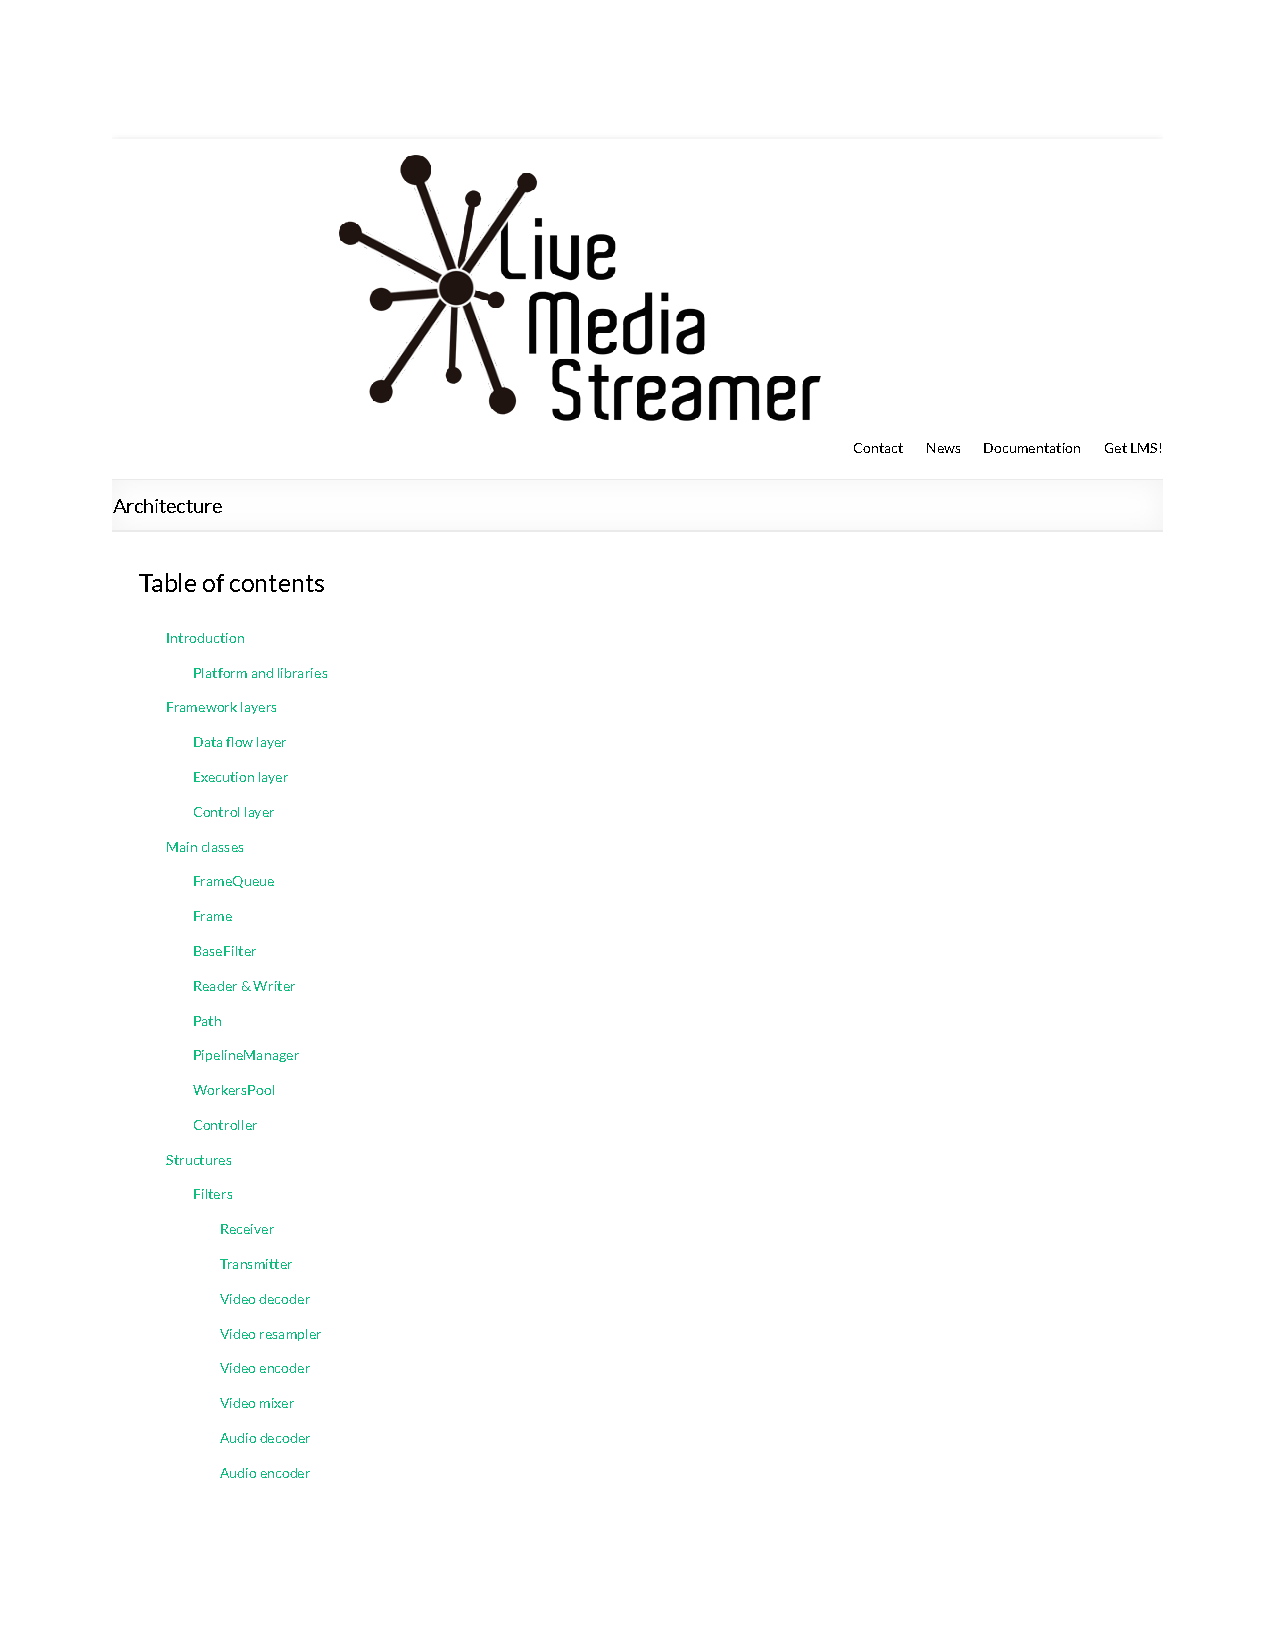
\includepdf[pages=-]{./appendix/lmsArchPrint.pdf}
\chapter{LMS HTTP RESTful API}\label{ANX:RESTAPI}

Proposed HTTP RESTful API's structure for managing an instance of the LiveMediaStreamer:

\begin{itemize}
\item Generic management queries
\begin{itemize}
\item Connect \hfill

Checks if an existing instance of LMS is running and sets the LMS port and LMS host to work with.
\begin{quote}
\begin{verbatim}
POST http://<host>:<port>/api/connect
JSON    {
            "port":<lms-port>,
            "host":"<lms-host>"
        }
\end{verbatim}
\end{quote}
\item Disconnect \hfill

Resets the running LMS instance and sets \verb|lms-port| and \verb|lms-host| to null in order to connect again to the same or any another LMS instance running.
\begin{quote}
\begin{verbatim}
GET http://<host>:<port>/api/disconnect
\end{verbatim}
\end{quote}
\item State \hfill

Gets the state object of the current LMS instance connected to (JSON object with the configured filters and paths).
\begin{quote}
\begin{verbatim}
GET http://<host>:<port>/api/state
\end{verbatim}
\end{quote}
\item Create a filter \hfill

Creates a filter (current types are: receiver, transmitter, demuxer, dasher, audioDecoder, audioEncoder, videoDecoder, videoResampler, videoEncoder, audioMixer, videoMixer) with an unique identifier.
\begin{quote}
\begin{verbatim}
POST http://<host>:<port>/api/createFilter
JSON    {
            "id": filterID,
            "type": "type"
        }
\end{verbatim}
\end{quote}        
\item Create a path of filters \hfill

Create a path of filters. A path can be a master path or an slave one, as shown:

\begin{itemize}

\item Master path
\begin{quote}
\begin{verbatim}
POST http://<host>:<port>/api/createPath
JSON    { 
            'id' : pathId, 
            'orgFilterId' : orgFilterId, 
            'dstFilterId' : dstFilterId, 
            'orgWriterId' : orgWriterId, 
            'dstReaderId' : dstReaderId, 
            'midFiltersIds' : [filterID1, filterID2,...] 
        }
\end{verbatim}
\end{quote}
\item Slave path of previous master path
\begin{quote}
\begin{verbatim}
POST http://<host>:<port>/api/createPath
JSON    { 
            'id' : pathId, 
            'orgFilterId' : filterID1, 
            'dstFilterId' : dstFilterId2, 
            'orgWriterId' : -1, 
            'dstReaderId' : dstReaderId2, 
            'midFiltersIds' : [filterID3, filterID4,...] 
        }  
\end{verbatim}
\end{quote}
\end{itemize}
\end{itemize}
\item Specific filter management queries        
\begin{itemize}
\item Configure an existing filter \hfill

Configures an existing filter (each filter has its own actions defined, check APPENDIX \ref{ANX:lmsarchfull})
\begin{quote}
\begin{verbatim}
PUT http://<host>:<port>/api/filter/:filterID
JSON    [
            {
                "action":"the action",
                    "params":{
                        "param1":param1,
                        "param2":"param2",
                        "param3":"param3",
                        "param4":true
                }
            }
        ]
\end{verbatim}
\end{quote}

\end{itemize}
\end{itemize}

So, with previous API proposal, the whole LMS's TCP socket API becomes simplified.

Moreover, specific responses format to client has been proposed as shown:

\begin{itemize}
\item Success messages \hfill

It may be a string, bool, array or another object, depending on the request method

\begin{quote}
\begin{verbatim}
JSON    {
            "message": { the incoming message }
        }
\end{verbatim}
\end{quote}        
\item Error messages \hfill

\begin{quote}
\begin{verbatim}
JSON    {
            "error": "the error message"
        }
\end{verbatim}
\end{quote}
\end{itemize}
\chapter{Specific application metric methods}\label{ANX:appALG}

This appendix is showing concrete algorithm of interest in order to help understanding how application methods work.

\section{Input network metric method}\label{inmm}
\begin{quote}
\begin{verbatim}
void SCSSubsessionStats::
			periodicStatMeasurement(struct timeval const& timeNow) 
{
    unsigned secsDiff = timeNow.tv_sec - measurementEndTime.tv_sec;
    int usecsDiff = timeNow.tv_usec - measurementEndTime.tv_usec;
    double timeDiff = secsDiff + usecsDiff/1000000.0;
    measurementEndTime = timeNow;

    RTPReceptionStatsDB::Iterator statsIter(fSource->receptionStatsDB());

    RTPReceptionStats* stats = statsIter.next(True);
    if (stats != NULL) {
        double kBytesTotalNow = stats->totNumKBytesReceived();
        double kBytesDeltaNow = kBytesTotalNow - kBytesTotal;
        kBytesTotal = kBytesTotalNow;

        double kbpsNow = timeDiff == 0.0 ? 0.0 : 8*kBytesDeltaNow/timeDiff;
        if (kbpsNow < 0.0) kbpsNow = 0.0; // in case of roundoff error
        if (kbpsNow < kbitsPerSecondMin) kbitsPerSecondMin = kbpsNow;
        if (kbpsNow > kbitsPerSecondMax) kbitsPerSecondMax = kbpsNow;

        unsigned totReceivedNow = stats->totNumPacketsReceived();
        unsigned totExpectedNow = stats->totNumPacketsExpected();
        unsigned deltaReceivedNow = totReceivedNow - totNumPacketsReceived;
        unsigned deltaExpectedNow = totExpectedNow - totNumPacketsExpected;
        totNumPacketsReceived = totReceivedNow;
        totNumPacketsExpected = totExpectedNow;

        double lossFractionNow = deltaExpectedNow == 0 ? 0.0 : 1.0 -
        							 deltaReceivedNow/(double)deltaExpectedNow;

        if (lossFractionNow < packetLossFractionMin) {
            packetLossFractionMin = lossFractionNow;
        }
        if (lossFractionNow > packetLossFractionMax) {
            packetLossFractionMax = lossFractionNow;
        }

        minInterPacketGapUS = stats->minInterPacketGapUS();
        maxInterPacketGapUS = stats->maxInterPacketGapUS();
        totalGaps = stats->totalInterPacketGaps();
        jitter = stats->jitter();
    }
}
\end{verbatim}
\end{quote} 
\section{Output network metric method}\label{onmm}


\begin{quote}
\begin{verbatim}
void ConnRTCPInstance::
			periodicStatMeasurement(struct timeval const& timeNow) 
{
    unsigned currentNumBytes;
    double currentElapsedTime;

    RTPTransmissionStatsDB::Iterator 
    							statsIter(fSink->transmissionStatsDB());

    fSink->getTotalBitrate(currentNumBytes, currentElapsedTime);

    avgBitrate = currentElapsedTime == 0 ? 0.0 :
    					((8*currentNumBytes/currentElapsedTime)/1000.0);
    if(minBitrate > avgBitrate) minBitrate = avgBitrate;
    if(maxBitrate < avgBitrate) maxBitrate = avgBitrate;

    RTPTransmissionStats* stats;
    while((stats = statsIter.next()) != NULL){
        SSRC = stats->SSRC();
        packetLossRatio = stats->packetLossRatio();
        if(minPacketLossRatio > packetLossRatio) 
        							minPacketLossRatio = packetLossRatio;
        if(maxPacketLossRatio < packetLossRatio) 
        							maxPacketLossRatio = packetLossRatio;        
        
        roundTripDelay = stats->roundTripDelay();
        if(minRoundTripDelay > roundTripDelay) 
        							minRoundTripDelay = roundTripDelay;
        if(maxRoundTripDelay < roundTripDelay) 
        							maxRoundTripDelay = roundTripDelay;

        jitter = stats->jitter();
        if(minJitter > jitter) minJitter = jitter;
        if(maxJitter < jitter) maxJitter = jitter;
    }
}
\end{verbatim}
\end{quote} 
\section{Pipiline delay metric method}\label{pdmm}


\begin{quote}
\begin{verbatim}
void Reader::measureDelay()
{
    if(lastTs.count() < 0){
        lastTs = frame->getPresentationTime();
    }

    if (lastTs == frame->getPresentationTime()) {
        return;
    }

    timeCounter += frame->getPresentationTime() - lastTs;
    lastTs = frame->getPresentationTime();

    if(timeCounter >= windowDelay){
        avgDelay = delay / frameCounter;
        timeCounter = std::chrono::microseconds(0);
        delay = std::chrono::microseconds(0);
        frameCounter = 0;
    }
    
    delay += std::chrono::duration_cast<std::chrono::
    						microseconds>(std::chrono::system_clock::now() 
    											- frame->getOriginTime());
    frameCounter++;
}
\end{verbatim}
\end{quote} 


\chapter{Docker cheat sheet}\label{ANX:csd}

This is a continually expanded GitHub repository where Docker users contribute with specific usages of the Docker technology:

\href{https://github.com/wsargent/docker-cheat-sheet}{Docker cheat sheet}

Current version of previous Docker cheat sheet is attached within next pages:

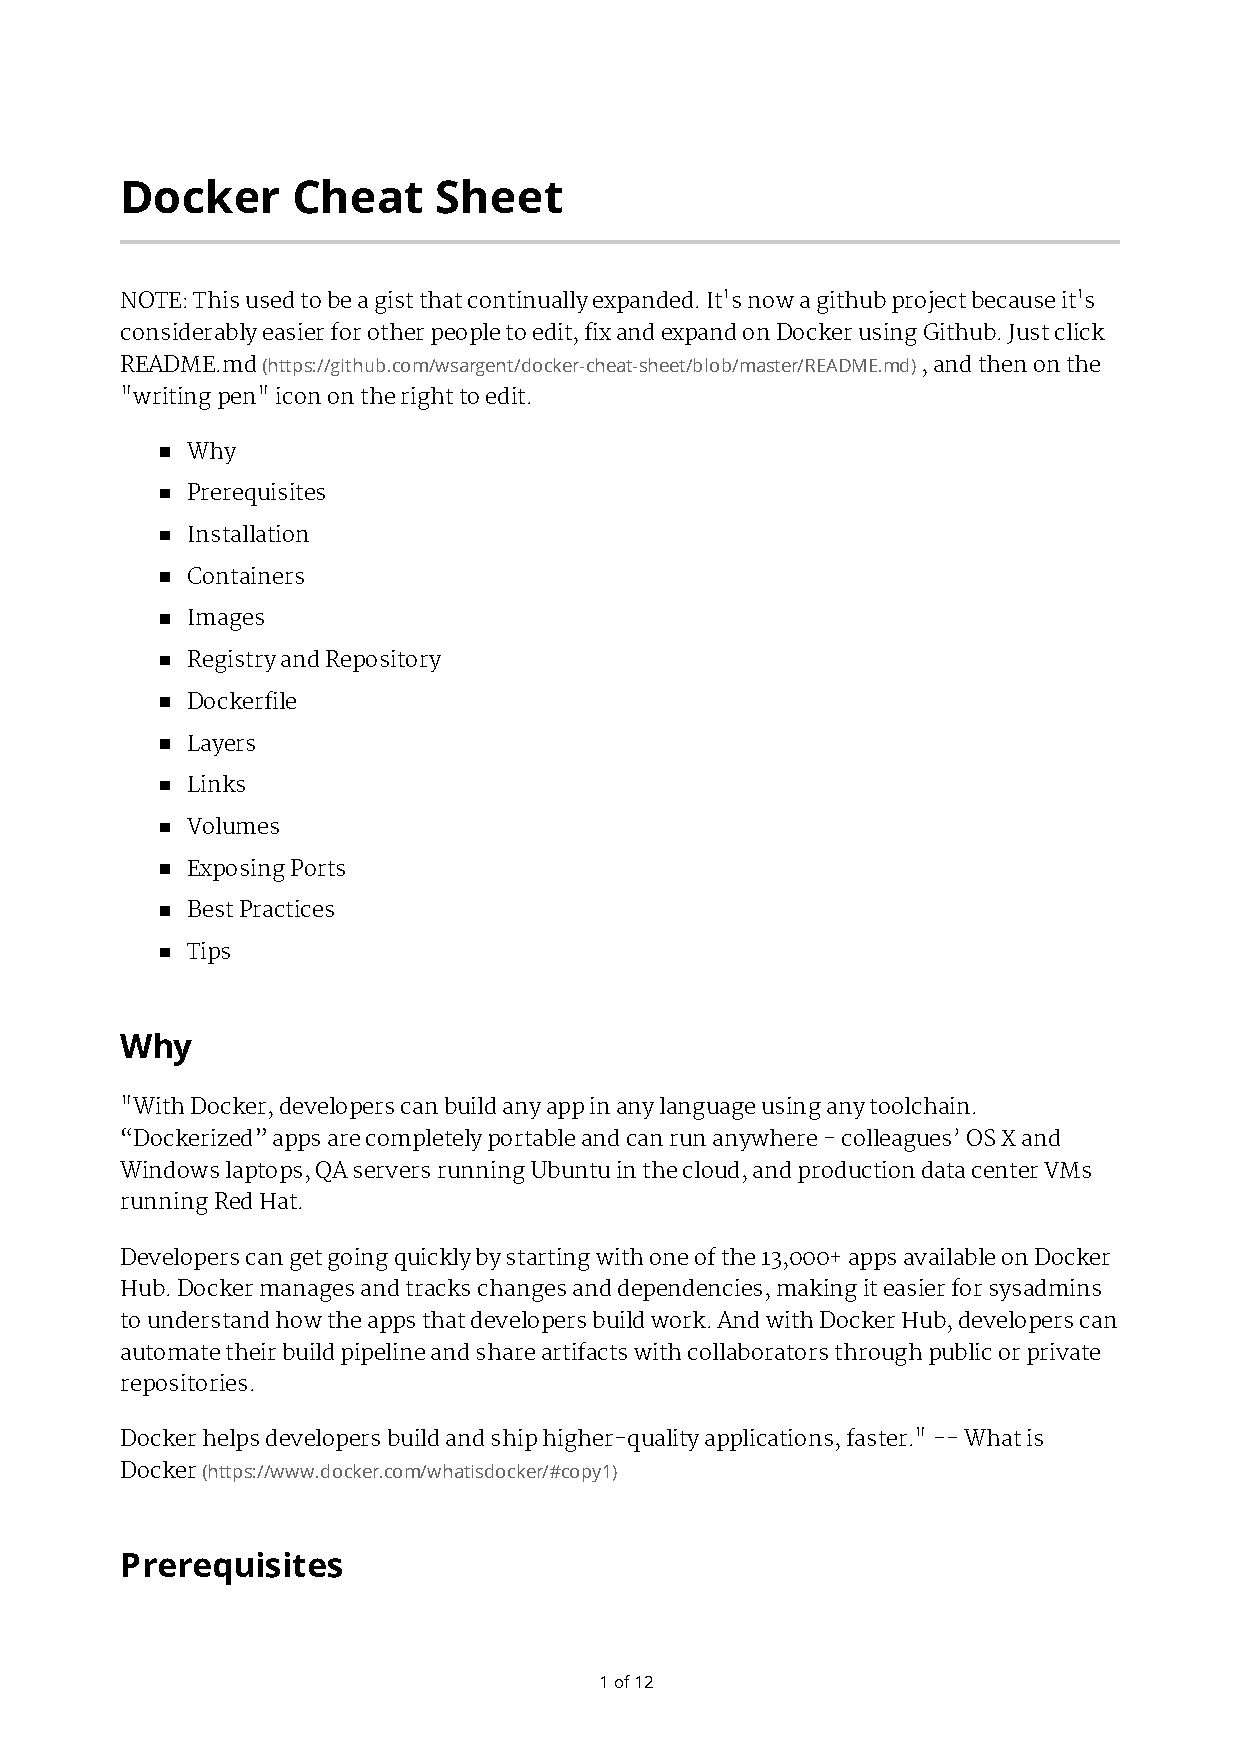
\includepdf[pages=-]{./appendix/wsargent-docker-cheat-sheet-blob-master-README.pdf}
\chapter{Docker, Nginx and Collectd configuration files}\label{ANX:dockerFiles}

This appendix is listing specific Docker, Nginx and Collectd configuration files.

\section{Basic LMS container}\label{ANX:dockerFiles1}

\begin{verbatim}
# LiveMediaStreamer Container
FROM ubuntu:14.04
MAINTAINER Gerard CL <gerardcl@gmail.com>

RUN apt-get update && apt-get -y upgrade

RUN apt-get -y install git cmake autoconf automake build-essential \ 
libass-dev libtheora-dev libtool libvorbis-dev pkg-config zlib1g-dev \
libcppunit-dev yasm libx264-dev  libmp3lame-dev  libopus-dev \
libvpx-dev liblog4cplus-dev libtinyxml2-dev opencv-data \
libopencv-dev mercurial cmake-curses-gui vim libcurl3 wget curl 

RUN adduser --disabled-password --gecos '' lms && adduser lms sudo \
	&& echo '%sudo ALL=(ALL) NOPASSWD:ALL' >> /etc/sudoers

USER lms

RUN hg clone https://bitbucket.org/multicoreware/x265 /home/lms/x265 \
	&& cd /home/lms/x265 && cmake -G "Unix Makefiles" ./source \
	&& make -j && sudo make install && sudo ldconfig

RUN git clone https://github.com/mstorsjo/fdk-aac.git/ /home/lms/fdk-aac \
	&& cd /home/lms/fdk-aac && libtoolize && ./autogen.sh \
	&& ./configure && make -j && sudo make install && sudo ldconfig

RUN cd /home/lms && wget http://ffmpeg.org/releases/ffmpeg-2.7.tar.bz2 \
	&& tar xjvf ffmpeg-2.7.tar.bz2 && cd ffmpeg-2.7 \
	&& ./configure --enable-gpl --enable-libass --enable-libtheora \
	--enable-libvorbis --enable-libx264 --enable-nonfree --enable-shared \
	--enable-libopus --enable-libmp3lame --enable-libvpx \
	--enable-libfdk_aac --enable-libx265 && make -j \
	&& sudo make install && sudo ldconfig

RUN cd /home/lms && wget \
	http://www.live555.com/liveMedia/public/live555-latest.tar.gz \
	&& tar xaf live555-latest.tar.gz && cd live \
	&& ./genMakefiles linux-with-shared-libraries && make -j \
	&& sudo make install && sudo ldconfig

RUN git clone https://github.com/ua-i2cat/livemediastreamer.git \
	/home/lms/livemediastreamer && cd /home/lms/livemediastreamer \
	&& git checkout development && ./autogen.sh \
	&& make -j && sudo make install && sudo ldconfig

EXPOSE 5000-5017/udp
EXPOSE 8554-8564
EXPOSE 7777

CMD ["/usr/local/bin/livemediastreamer","7777"] 
\end{verbatim}

\section{HTTP REST API container}\label{ANX:dockerFiles2}

\begin{verbatim}
# LiveMediaStreamer Container
FROM ubuntu:14.04

MAINTAINER Gerard CL <gerardcl@gmail.com>

RUN apt-get update && apt-get -y upgrade

RUN apt-get -y install git npm

RUN adduser --disabled-password --gecos '' lms \
&& adduser lms sudo \
&& echo '%sudo ALL=(ALL) NOPASSWD:ALL' >> /etc/sudoers

USER lms

RUN cd /home/lms \
&& git clone https://github.com/ua-i2cat/LMStoREST.git \
/home/lms/LMStoREST && cd /home/lms/LMStoREST && npm install

EXPOSE 8080
CMD ["nodejs", "/home/lms/LMStoREST/lms-middleware.js"]
\end{verbatim}

\section{Running multiple processes within a container}\label{ANX:dockerFiles3}

\begin{verbatim}
# LiveMediaStreamer Container
# and Nginx server for MPEG-DASH streaming
FROM ubuntu:14.04
MAINTAINER Gerard CL <gerardcl@gmail.com>

RUN apt-get update && apt-get -y upgrade

RUN apt-get -y install git cmake autoconf automake build-essential \ 
libass-dev libtheora-dev libtool libvorbis-dev pkg-config zlib1g-dev \
libcppunit-dev yasm libx264-dev  libmp3lame-dev  libopus-dev \
libvpx-dev liblog4cplus-dev libtinyxml2-dev opencv-data \
libopencv-dev mercurial cmake-curses-gui vim libcurl3 wget curl 

RUN apt-get -y install nginx supervisor
RUN mkdir -p /var/lock/nginx /var/run/nginx \
	/var/lock/livemediastreamer /var/run/livemediastreamer \
	/var/log/supervisor

ADD ./nginx.conf /etc/nginx/nginx.conf
ADD ./supervisord.conf /etc/supervisor/conf.d/supervisord.conf


RUN adduser --disabled-password --gecos '' lms \
&& adduser lms sudo \
&& echo '%sudo ALL=(ALL) NOPASSWD:ALL' >> /etc/sudoers

RUN mkdir -p /home/lms/dashSegments

USER lms

RUN hg clone https://bitbucket.org/multicoreware/x265 /home/lms/x265 \
	&& cd /home/lms/x265 && cmake -G "Unix Makefiles" ./source \
	&& make -j && sudo make install && sudo ldconfig

RUN git clone https://github.com/mstorsjo/fdk-aac.git/ /home/lms/fdk-aac \
	&& cd /home/lms/fdk-aac && libtoolize && ./autogen.sh \
	&& ./configure && make -j && sudo make install && sudo ldconfig

RUN cd /home/lms && wget http://ffmpeg.org/releases/ffmpeg-2.7.tar.bz2 \
	&& tar xjvf ffmpeg-2.7.tar.bz2 && cd ffmpeg-2.7 \
	&& ./configure --enable-gpl --enable-libass --enable-libtheora \
	--enable-libvorbis --enable-libx264 --enable-nonfree --enable-shared \
	--enable-libopus --enable-libmp3lame --enable-libvpx \
	--enable-libfdk_aac --enable-libx265 && make -j \
	&& sudo make install && sudo ldconfig

RUN cd /home/lms && wget \
	http://www.live555.com/liveMedia/public/live555-latest.tar.gz \
	&& tar xaf live555-latest.tar.gz && cd live \
	&& ./genMakefiles linux-with-shared-libraries && make -j \
	&& sudo make install && sudo ldconfig

RUN git clone https://github.com/ua-i2cat/livemediastreamer.git \
	/home/lms/livemediastreamer && cd /home/lms/livemediastreamer \
	&& git checkout development && ./autogen.sh \
	&& make -j && sudo make install && sudo ldconfig

USER root

EXPOSE 5000-5017/udp
EXPOSE 8554-8564
EXPOSE 7777
EXPOSE 8080

CMD ["/usr/bin/supervisord"] 
\end{verbatim}

\section{Nginx server file configuration example}\label{ANX:nginxexample}

\begin{verbatim}
# this sets the user nginx will run as, 
# and the number of worker processes
user nobody nogroup;
worker_processes  1;

# setup where nginx will log errors to 
# and where the nginx process id resides
error_log  /var/log/nginx/error.log;
pid        /var/run/nginx.pid;

events {
  worker_connections  1024;
  # set to on if you have more than 1 worker_processes 
  accept_mutex off;
}

http {
  include       /etc/nginx/mime.types;

  default_type application/octet-stream;
  access_log /tmp/nginx.access.log combined;
 
  # use the kernel sendfile
  sendfile        on;
  # prepend http headers before sendfile() 
  tcp_nopush     on;

  keepalive_timeout  5;
  tcp_nodelay        on;

  gzip  on;
  gzip_vary on;
  gzip_min_length 500;
  
  gzip_disable "MSIE [1-6]\.(?!.*SV1)";
  gzip_types text/plain text/xml text/css
     text/comma-separated-values
     text/javascript application/x-javascript
     application/atom+xml image/x-icon;

  # configure the virtual host
  server {
    # replace with your domain name
    server_name localhost;
    root /home/lms/dashSegments;
    # port to listen for requests on
    listen 8090;
    # maximum accepted body size of client request 
    client_max_body_size 4G;
    # the server will close connections after this time 
    keepalive_timeout 5;
    
    add_header Access-Control-Allow-Origin "*";
    add_header Access-Control-Allow-Methods "GET, OPTIONS";
    add_header Access-Control-Allow-Headers "origin, authorization, accept";
    add_header Cache-Control no-cache;
    
    location / {
        add_header Access-Control-Allow-Origin "*";
        add_header Access-Control-Allow-Methods "GET, OPTIONS";
        add_header Access-Control-Allow-Headers "origin, authorization, accept";
        add_header Cache-Control no-cache;
    }
  }
}

daemon off;
\end{verbatim}

\section{Sharing volumes within containers}\label{ANX:dockerFiles4}
\begin{verbatim}
# Nginx Container - LMS special one
FROM ubuntu:14.04
MAINTAINER Gerard CL <gerardcl@gmail.com>

RUN apt-get update && apt-get install --fix-missing \
	&& apt-get -y upgrade

RUN apt-get -y install nginx 

ADD ./nginx.conf /etc/nginx/nginx.conf

RUN adduser --disabled-password --gecos '' lms \
	&& adduser lms sudo \
	&& echo '%sudo ALL=(ALL) NOPASSWD:ALL' >> /etc/sudoers

RUN mkdir -p /home/lms/dashSegments

EXPOSE 8090

CMD ["/usr/sbin/nginx"]  
\end{verbatim}

\section{Collectd client container}\label{ANX:dockerFiles5}

\begin{verbatim}

FROM    ubuntu:14.04
MAINTAINER Gerard CL <gerardcl@gmail.com>

ENV     DEBIAN_FRONTEND noninteractive

RUN apt-get update
RUN apt-get -y install collectd curl python-dev python-pip

ADD collectd.conf.tpl /etc/collectd/collectd.conf.tpl

RUN pip install envtpl
ADD start_container /usr/bin/start_container
RUN chmod +x /usr/bin/start_container
CMD start_container

\end{verbatim}

\section{Collectd client configuration}\label{ANX:collectdFiles1}

\begin{verbatim}
Hostname "{{ LMS_NAME }}"
FQDNLookup true

Interval 1
Timeout 4
ReadThreads 5

LoadPlugin syslog
LoadPlugin cpu
LoadPlugin load
LoadPlugin memory
LoadPlugin network

<Plugin "syslog">
  LogLevel "info"
  NotifyLevel "OKAY"
</Plugin>

<Plugin network>
  Server "{{ GRAPHITE_HOST }}" "{{ GRAPHITE_PORT | default("25826") }}"
  ReportStats true
</Plugin>
\end{verbatim}

\section{Collectd server and Graphite container}\label{ANX:dockerFiles6}


\begin{verbatim}
# LiveMediaStreamer Container
FROM ubuntu:14.04
MAINTAINER Gerard CL <gerardcl@gmail.com>

RUN apt-get update
RUN apt-get install -y python-cairo collectd-core libgcrypt11 \
python-virtualenv build-essential python-dev supervisor sudo

RUN adduser --system --group --no-create-home collectd \
&& adduser --system --home /opt/graphite graphite

RUN sudo -u graphite virtualenv --system-site-packages ~graphite/env

RUN echo "django \n \
  python-memcached \n \
  django-tagging \n \
  twisted \n \
  gunicorn \n \
  whisper \n \
  carbon \n \
  graphite-web" > /tmp/graphite_reqs.txt

RUN sudo -u graphite HOME=/opt/graphite /bin/sh -c ". \
~/env/bin/activate && pip install -r /tmp/graphite_reqs.txt"

ADD collectd/collectd.conf /etc/collectd/
ADD supervisor/ /etc/supervisor/conf.d/
ADD graphite/settings.py /opt/graphite/webapp/graphite/
ADD graphite/local_settings.py /opt/graphite/webapp/graphite/
ADD graphite/mkadmin.py /opt/graphite/webapp/graphite/
ADD graphite/storage-schemas.conf /opt/graphite/conf/

RUN cp /opt/graphite/conf/carbon.conf.example \
/opt/graphite/conf/carbon.conf
RUN cp /opt/graphite/conf/graphite.wsgi.example \
/opt/graphite/webapp/graphite/graphite_wsgi.py
RUN cp /opt/graphite/conf/graphite.wsgi.example \
/opt/graphite/conf/graphite.wsgi
RUN cp /opt/graphite/conf/storage-aggregation.conf.example \
/opt/graphite/conf/storage-aggregation.conf

RUN sed -i "s#^\(SECRET_KEY = \).*#\1\"`python -c 'import os; import base64; \
print(base64.b64encode(os.urandom(40)))'`\"#" \
/opt/graphite/webapp/graphite/app_settings.py
RUN sudo -u graphite HOME=/opt/graphite PYTHONPATH=/opt/graphite/lib/ \
/bin/sh -c "cd ~/webapp/graphite && ~/env/bin/python manage.py syncdb --noinput"
RUN sudo -u graphite HOME=/opt/graphite PYTHONPATH=/opt/graphite/lib/ \
/bin/sh -c "cd ~/webapp/graphite && ~/env/bin/python mkadmin.py"

EXPOSE 8080 25826/udp

CMD exec supervisord -n
\end{verbatim}

\section{Collectd server configuration}\label{ANX:collectdFiles2}

\begin{verbatim}
Hostname "localhost"
FQDNLookup true
Interval 1

LoadPlugin syslog
LoadPlugin network
LoadPlugin write_graphite

<Plugin syslog>
	LogLevel "info"
	NotifyLevel "OKAY"
</Plugin>

<Plugin network>
	Listen "*" "25826"
	ReportStats true
</Plugin>

<Plugin write_graphite>
	<Node "graphing">
		Host "localhost"
		Port "2003"
		Protocol "tcp"
		LogSendErrors true
		Prefix "collectd."
		StoreRates true
		AlwaysAppendDS false
		EscapeCharacter "_"
	</Node>
</Plugin>
\end{verbatim}

\section{Collectd tail plugin example configuration}\label{ANX:collectdTailFiles2}

Next tail plugin configuration is performing specific regular expression matching to bind logged metrics from the LMS demo script. Each logged line to stdout is formatted as shown next:

\begin{verbatim}
|PATHID|value|avgDelay-5004|value|lostBlocs-5004|value|PATHID|value
|avgDelay-5006|value|lostBlocs-5006|value|RXmediaType|video
|videoRXavgBitRateInKbps|value|videoRXavgPacketLossPercentage
|value|videoRXavgInterPacketGapInMiliseconds|value
|videoRXcurJitterInMicroseconds|value|RXmediaType|audio
|audioRXavgBitRateInKbps|value|audioRXavgPacketLossPercentage
|value|audioRXavgInterPacketGapInMiliseconds|value
|audioRXcurJitterInMicroseconds|value|TX_URI|value
|TX_SSRC-1|value|TXavgBitrateInKbps-1|value
|TXpacketLossRatio-1|value|TXjitterInMicroseconds-1
|value|TXroundTripDelayMilliseconds-1|value|TX_SSRC-2
|value|TXavgBitrateInKbps-2|value|TXpacketLossRatio-2
|value|TXjitterInMicroseconds-2|value|TXroundTripDelayMilliseconds-2|value|
\end{verbatim}

Then, each new line is parsed through the tail plugin of the Collectd configuration. An example is shown next:
\begin{verbatim}
<Plugin tail>
<File "/home/lms/logs/lms.log">
Instance "lmsTest"
<Match>
Regex ".*avgDelay-5004\\|([0-9]*).*"
DSType "CounterAdd"
Type counter
Instance "VideoAVGdelay-us"
</Match>
<Match>
Regex ".*lostBlocs-5004\\|([0-9]*).*"
DSType "CounterAdd"
Type counter
Instance "VideoLostBlocs"
</Match>
<Match>
Regex ".*avgDelay-5006\\|([0-9]*).*"
DSType "CounterAdd"
Type counter
Instance "AudioAVGdelay-us"
</Match>
<Match>
Regex ".*lostBlocs-5006\\|([0-9]*).*"
DSType "CounterAdd"
Type counter
Instance "AudioLostBlocs"
</Match>
<Match>
Regex ".*RXmediaType\\|video.*videoRXavgBitRateInKbps\\|([0-9]*).*"
DSType "CounterAdd"
Type counter
Instance "videoRXavgBitRateInKbps"
</Match>
<Match>
Regex ".*RXmediaType\\|video.*videoRXavgPacketLossPercentage\\|([0-9]*).*"
DSType "CounterAdd"
Type counter
Instance "videoRXavgPacketLossPercentage"
</Match>
<Match>
Regex ".*RXmediaType\\|video.*videoRXavgInterPacketGapInMiliseconds\\|([0-9]*).*"
DSType "CounterAdd"
Type counter
Instance "videoRXavgInterPacketGapInMiliseconds"
</Match>
<Match>
Regex ".*RXmediaType\\|video.*videoRXcurJitterInMicroseconds\\|([0-9]*).*"
DSType "CounterAdd"
Type counter
Instance "videoRXcurJitterInMicroseconds"
</Match>
<Match>
Regex ".*RXmediaType\\|audio.*audioRXavgBitRateInKbps\\|([0-9]*).*"
DSType "CounterAdd"
Type counter
Instance "audioRXavgBitRateInKbps"
</Match>
<Match>
Regex ".*RXmediaType\\|audio.*audioRXavgPacketLossPercentage\\|([0-9]*).*"
DSType "CounterAdd"
Type counter
Instance "audioRXavgPacketLossPercentage"
</Match>
<Match>
Regex ".*RXmediaType\\|audio.*audioRXavgInterPacketGapInMiliseconds\\|([0-9]*).*"
DSType "CounterAdd"
Type counter
Instance "audioRXavgInterPacketGapInMiliseconds"
</Match>
<Match>
Regex ".*RXmediaType\\|audio.*audioRXcurJitterInMicroseconds\\|([0-9]*).*"
DSType "CounterAdd"
Type counter
Instance "audioRXcurJitterInMicroseconds"
</Match>
<Match>
Regex ".*TXavgBitrateInKbps-1\\|([0-9]*).*"
DSType "CounterAdd"
Type counter
Instance "VideoTXavgBitrateInKbps"
</Match>
<Match>
Regex ".*TXpacketLossRatio-1\\|([0-9]*).*"
DSType "CounterAdd"
Type counter
Instance "VideoTXpacketLossRatio"
</Match>
<Match>
Regex ".*TXjitterInMicroseconds-1\\|([0-9]*).*"
DSType "CounterAdd"
Type counter
Instance "VideoTXjitterInMicroseconds"
</Match>
<Match>
Regex ".*TXroundTripDelayMilliseconds-1\\|([0-9]*).*"
DSType "CounterAdd"
Type counter
Instance "VideoTXroundTripDelayMilliseconds"
</Match>
<Match>
Regex ".*TXavgBitrateInKbps-2\\|([0-9]*).*"
DSType "CounterAdd"
Type counter
Instance "AudioTXavgBitrateInKbps"
</Match>
<Match>
Regex ".*TXpacketLossRatio-2\\|([0-9]*).*"
DSType "CounterAdd"
Type counter
Instance "AudioTXpacketLossRatio"
</Match>
<Match>
Regex ".*TXjitterInMicroseconds-2\\|([0-9]*).*"
DSType "CounterAdd"
Type counter
Instance "AudioTXjitterInMicroseconds"
</Match>
<Match>
Regex ".*TXroundTripDelayMilliseconds-2\\|([0-9]*).*"
DSType "CounterAdd"
Type counter
Instance "AudioTXroundTripDelayMilliseconds"
</Match>
</File>
</Plugin>
\end{verbatim}

\chapter{Source codes}\label{ANX:sourceCodes}

Full source codes can be found in the GitHub's web page of the Media Internet Area's developers team of the i2CAT Foundation:

\begin{itemize}
\item \href{https://github.com/ua-i2cat/LMStoREST}{HTTP REST API} \hfill

This is the source code repository for the RESTfull API middleware.\hfill

\url{https://github.com/ua-i2cat/LMStoREST}

\item \href{https://github.com/ua-i2cat/liveMediaStreamer}{LiveMediaStreame framework} \hfill

This is the source code repository for the LiveMediaStreamer framework. \hfill

\url{https://github.com/ua-i2cat/liveMediaStreamer}

Concretely:
\begin{itemize}
\item \href{https://github.com/ua-i2cat/liveMediaStreamer/tree/development/src/modules/liveMediaInput}{Statistics for network inputs} \hfill

\url{https://github.com/ua-i2cat/liveMediaStreamer/tree/development/src/modules/liveMediaInput}

\item \href{https://github.com/ua-i2cat/liveMediaStreamer/tree/development/src/modules/liveMediaOutput}{Statistics for network outputs} \hfill

\url{https://github.com/ua-i2cat/liveMediaStreamer/tree/development/src/modules/liveMediaOutput}
\item \href{https://github.com/ua-i2cat/liveMediaStreamer/blob/development/src/IOInterface.cpp}{Statistics for pipeline metrics} \hfill

\url{https://github.com/ua-i2cat/liveMediaStreamer/blob/development/src/IOInterface.cpp}
\end{itemize}


\end{itemize}


\chapter{Exchanged e-mails with Live555 developer mailing list}\label{emailRoss}

E-mail sent:

\begin{quote}
\begin{verbatim}
Sender: Gerard Castillo Lasheras <gerard.castillo@i2cat.net>
Receiver: LIVE555 Streaming Media - development & 
									use <live-devel@ns.live555.com> 
Hi Ross,

I'm implementing statistics on our software (liveMediaStreamer framework) 
and I'd like to have access to the RTPTransmissionStatsDB. But, I do not
see how to get the RTPSink object (which has the RTPTransmissionStatsDB 
and its stats).

Which should be the proper way to get the RTPSink object related to my
OnDemandServerMediaSubsession childs? I've seen that 
OnDemandServerMediaSubsession has a friend classe StreamState 
which has the RTPSink associated but, anyway, 
I'm not able to have access to it.

Thanks in advance,

Kind regards,
\end{verbatim}
\end{quote} 

The reply:
\begin{quote}
\begin{verbatim}
Sender: Ross Finlayson <finlayson@live555.com>
Receiver: LIVE555 Streaming Media - development & 
									use <live-devel@ns.live555.com> 
									
First of all, note that while a "OnDemandServerMediaSubsession" 
object refers to a track of streamable media, a "RTPSink" object 
refers to a receiving client (or possibly multiple clients if 
"reuseFirstSource" is True).  So there’s (in general) a 
one-to-many relationship between "OnDemandServerMediaSubsession" 
and "RTPSink".  Thus, it doesn’t make sense to talk about 
*the* RTPSink object for your "OnDemandServerMediaSubsession".

However…
There are at least two possible ways to get access to the 
"RTPSink" objects:

1/ Note the pure virtual function "createNewRTPSink()" that you 
have implemented in your "OnDemandServerMediaSubsession" subclass.  
You can use your implementation of this function to get access 
to the "RTPTransmissionStatsDB" for the new "RTPSink", after 
you’ve created it.
The drawback of this approach, though, is that you don’t know when 
the "RTPSink" object later gets deleted, so - if you’re not 
careful - you may end up holding a reference or pointer to a 
"RTPTransmissionStatsDB" that has been deleted.

2/ Define a subclass "myRTCPInstance" of the "RTCPInstance" 
class.  Then, in your "OnDemandServerMediaSubsession" subclass, 
reimplement the "createRTCP()" virtual function to create a 
"myRTCPInstance" object, rather than a "RTCPInstance" 
object.  Note that "createRTCP()" contains a "sink" 
parameter, pointing to a "RTPSink", from which you can 
get the "RTPTransmissionStatsDB".
The advantage of this approach over approach 1/ is that 
- by defining a subclass of "RTCPInstance", you can learn when 
the "RTPInstance" object gets deleted, and thus when the 
"RTPSink" object gets deleted.  (The "RTCPInstance" object 
always gets deleted immediately before the "RTPSink" 
object.)  Thus, you can use your "myRTCPInstance" destructor 
to figure out when the "RTPTransmissionStatsDB" should no 
longer be used.
									
\end{verbatim}
\end{quote} 




%%%%%%%%%%%%%%%%%%%%%%%%%%%%%%%%%%%%%%%%%%%%%%%%%%%%%%%%%%%%%%%%%%%%%%%%%%
%%%%%%%%%%%%%%%%%%%%%%%%%%%%%%%%%%%%%%%%%%%%%%%%%%%%%%%%%%%%%%%%%%%%%%%%%%
%%%%%%%%%%%%%%%%%%%%%%%%%%%%%%%%%%%%%%%%%%%%%%%%%%%%%%%%%%%%%%%%%%%%%%%%%%
% i  aixo es tot! ;)
\end{document}





